% Options for packages loaded elsewhere
\PassOptionsToPackage{unicode,bookmarksdepth=0}{hyperref}
\PassOptionsToPackage{hyphens}{url}
\PassOptionsToPackage{dvipsnames,svgnames,x11names}{xcolor}
%
\documentclass[
  letterpaper,
  numbers=noendperiod,
  fontsize=11pt,
  DIV=12,
  titlepage=false]{scrreprt}

\usepackage{amsmath,amssymb}
\usepackage{setspace}
\usepackage{iftex}
\ifPDFTeX
  \usepackage[T1]{fontenc}
  \usepackage[utf8]{inputenc}
  \usepackage{textcomp} % provide euro and other symbols
\else % if luatex or xetex
  \usepackage{unicode-math}
  \defaultfontfeatures{Scale=MatchLowercase}
  \defaultfontfeatures[\rmfamily]{Ligatures=TeX,Scale=1}
\fi
\usepackage{lmodern}
\ifPDFTeX\else  
    % xetex/luatex font selection
\fi
% Use upquote if available, for straight quotes in verbatim environments
\IfFileExists{upquote.sty}{\usepackage{upquote}}{}
\IfFileExists{microtype.sty}{% use microtype if available
  \usepackage[]{microtype}
  \UseMicrotypeSet[protrusion]{basicmath} % disable protrusion for tt fonts
}{}
\makeatletter
\@ifundefined{KOMAClassName}{% if non-KOMA class
  \IfFileExists{parskip.sty}{%
    \usepackage{parskip}
  }{% else
    \setlength{\parindent}{0pt}
    \setlength{\parskip}{6pt plus 2pt minus 1pt}}
}{% if KOMA class
  \KOMAoptions{parskip=half}}
\makeatother
\usepackage{xcolor}
\usepackage[top=30mm,bottom=30mm,left=25mm,right=25mm]{geometry}
\setlength{\emergencystretch}{3em} % prevent overfull lines
\setcounter{secnumdepth}{3}
% Make \paragraph and \subparagraph free-standing
\makeatletter
\ifx\paragraph\undefined\else
  \let\oldparagraph\paragraph
  \renewcommand{\paragraph}{
    \@ifstar
      \xxxParagraphStar
      \xxxParagraphNoStar
  }
  \newcommand{\xxxParagraphStar}[1]{\oldparagraph*{#1}\mbox{}}
  \newcommand{\xxxParagraphNoStar}[1]{\oldparagraph{#1}\mbox{}}
\fi
\ifx\subparagraph\undefined\else
  \let\oldsubparagraph\subparagraph
  \renewcommand{\subparagraph}{
    \@ifstar
      \xxxSubParagraphStar
      \xxxSubParagraphNoStar
  }
  \newcommand{\xxxSubParagraphStar}[1]{\oldsubparagraph*{#1}\mbox{}}
  \newcommand{\xxxSubParagraphNoStar}[1]{\oldsubparagraph{#1}\mbox{}}
\fi
\makeatother


\providecommand{\tightlist}{%
  \setlength{\itemsep}{0pt}\setlength{\parskip}{0pt}}\usepackage{longtable,booktabs,array}
\usepackage{calc} % for calculating minipage widths
% Correct order of tables after \paragraph or \subparagraph
\usepackage{etoolbox}
\makeatletter
\patchcmd\longtable{\par}{\if@noskipsec\mbox{}\fi\par}{}{}
\makeatother
% Allow footnotes in longtable head/foot
\IfFileExists{footnotehyper.sty}{\usepackage{footnotehyper}}{\usepackage{footnote}}
\makesavenoteenv{longtable}
\usepackage{graphicx}
\makeatletter
\def\maxwidth{\ifdim\Gin@nat@width>\linewidth\linewidth\else\Gin@nat@width\fi}
\def\maxheight{\ifdim\Gin@nat@height>\textheight\textheight\else\Gin@nat@height\fi}
\makeatother
% Scale images if necessary, so that they will not overflow the page
% margins by default, and it is still possible to overwrite the defaults
% using explicit options in \includegraphics[width, height, ...]{}
\setkeys{Gin}{width=\maxwidth,height=\maxheight,keepaspectratio}
% Set default figure placement to htbp
\makeatletter
\def\fps@figure{htbp}
\makeatother
% definitions for citeproc citations
\NewDocumentCommand\citeproctext{}{}
\NewDocumentCommand\citeproc{mm}{%
  \begingroup\def\citeproctext{#2}\cite{#1}\endgroup}
\makeatletter
 % allow citations to break across lines
 \let\@cite@ofmt\@firstofone
 % avoid brackets around text for \cite:
 \def\@biblabel#1{}
 \def\@cite#1#2{{#1\if@tempswa , #2\fi}}
\makeatother
\newlength{\cslhangindent}
\setlength{\cslhangindent}{1.5em}
\newlength{\csllabelwidth}
\setlength{\csllabelwidth}{3em}
\newenvironment{CSLReferences}[2] % #1 hanging-indent, #2 entry-spacing
 {\begin{list}{}{%
  \setlength{\itemindent}{0pt}
  \setlength{\leftmargin}{0pt}
  \setlength{\parsep}{0pt}
  % turn on hanging indent if param 1 is 1
  \ifodd #1
   \setlength{\leftmargin}{\cslhangindent}
   \setlength{\itemindent}{-1\cslhangindent}
  \fi
  % set entry spacing
  \setlength{\itemsep}{#2\baselineskip}}}
 {\end{list}}
\usepackage{calc}
\newcommand{\CSLBlock}[1]{\hfill\break\parbox[t]{\linewidth}{\strut\ignorespaces#1\strut}}
\newcommand{\CSLLeftMargin}[1]{\parbox[t]{\csllabelwidth}{\strut#1\strut}}
\newcommand{\CSLRightInline}[1]{\parbox[t]{\linewidth - \csllabelwidth}{\strut#1\strut}}
\newcommand{\CSLIndent}[1]{\hspace{\cslhangindent}#1}

\usepackage{booktabs}
\usepackage{longtable}
\usepackage{array}
\usepackage{multirow}
\usepackage{wrapfig}
\usepackage{float}
\usepackage{colortbl}
\usepackage{pdflscape}
\usepackage{tabu}
\usepackage{threeparttable}
\usepackage{threeparttablex}
\usepackage[normalem]{ulem}
\usepackage{makecell}
\usepackage{xcolor}
% Compatibilidad caption/listings/etc. con KOMA (evita listas vacías o captions rotos)
\usepackage{scrhack}
\usepackage{booktabs}
\usepackage{longtable}
\usepackage{array}
\usepackage{float}
\usepackage{colortbl}
\usepackage{xcolor}
\usepackage{caption}
\usepackage{fancyhdr}
\captionsetup{font=small,labelfont=bf,skip=8pt,list=yes}
\renewcommand{\arraystretch}{1.2}

% Configuración de encabezados
\pagestyle{fancy}
\fancyhf{}
\fancyhead[LE,RO]{\thepage}
\fancyhead[LO]{\nouppercase{\leftmark}}
\fancyhead[RE]{\nouppercase{\rightmark}}
\renewcommand{\headrulewidth}{0.4pt}

% Pandoc inyecta otro \AtBeginDocument que vuelve a poner nombres en inglés;
% este hook corre al final de begin document y deja los títulos en español.
\AddToHook{begindocument/end}{%
  \renewcommand{\contentsname}{Índice General}%
  \renewcommand{\listfigurename}{Índice de Figuras}%
  \renewcommand{\listtablename}{Índice de Tablas}%
  \captionsetup{list=yes}%
}
% Sin encabezado en páginas preliminares
\AtBeginDocument{
  \pagenumbering{roman}
  \pagestyle{plain}
}

% Configuración para numeración continua de capítulos (las partes no cuentan)
\makeatletter
% Ocultar numeración de partes
\renewcommand{\thepart}{}
% Remover el reset automático de capítulos por parte para numeración continua
\@removefromreset{chapter}{part}
% Hacer que las secciones se numeren basándose en el capítulo, no en la parte
\@removefromreset{section}{part}
% Asegurar que las secciones se numeren dentro de cada capítulo
\renewcommand{\thesection}{\thechapter.\arabic{section}}
\makeatother

% Configuración para evitar saltos de página innecesarios
\clubpenalty=10000
\widowpenalty=10000
\displaywidowpenalty=10000

% Menos espacio en blanco antes del título de capítulo (empieza más arriba)
\makeatletter
\@ifundefined{chapter}{}{%
  \renewcommand*{\chapterheadstartvskip}{\vspace*{-2.5\baselineskip}}%
}
\makeatother
\KOMAoption{captions}{tableheading}
\makeatletter
\@ifpackageloaded{bookmark}{}{\usepackage{bookmark}}
\makeatother
\makeatletter
\@ifpackageloaded{caption}{}{\usepackage{caption}}
\AtBeginDocument{%
\ifdefined\contentsname
  \renewcommand*\contentsname{Table of contents}
\else
  \newcommand\contentsname{Table of contents}
\fi
\ifdefined\listfigurename
  \renewcommand*\listfigurename{List of Figures}
\else
  \newcommand\listfigurename{List of Figures}
\fi
\ifdefined\listtablename
  \renewcommand*\listtablename{List of Tables}
\else
  \newcommand\listtablename{List of Tables}
\fi
\ifdefined\figurename
  \renewcommand*\figurename{Figure}
\else
  \newcommand\figurename{Figure}
\fi
\ifdefined\tablename
  \renewcommand*\tablename{Table}
\else
  \newcommand\tablename{Table}
\fi
}
\@ifpackageloaded{float}{}{\usepackage{float}}
\floatstyle{ruled}
\@ifundefined{c@chapter}{\newfloat{codelisting}{h}{lop}}{\newfloat{codelisting}{h}{lop}[chapter]}
\floatname{codelisting}{Listing}
\newcommand*\listoflistings{\listof{codelisting}{List of Listings}}
\makeatother
\makeatletter
\makeatother
\makeatletter
\@ifpackageloaded{caption}{}{\usepackage{caption}}
\@ifpackageloaded{subcaption}{}{\usepackage{subcaption}}
\makeatother

\ifLuaTeX
  \usepackage{selnolig}  % disable illegal ligatures
\fi
\usepackage{bookmark}

\IfFileExists{xurl.sty}{\usepackage{xurl}}{} % add URL line breaks if available
\urlstyle{same} % disable monospaced font for URLs
\hypersetup{
  colorlinks=true,
  linkcolor={NavyBlue},
  filecolor={Maroon},
  citecolor={NavyBlue},
  urlcolor={NavyBlue},
  pdfcreator={LaTeX via pandoc}}


\author{}
\date{}

\begin{document}

% ============================================================================
% PORTADA - PRIMERA PÁGINA DEL DOCUMENTO
% ============================================================================
\thispagestyle{empty}
\begin{center}

\vspace*{0.2cm}

% Logo

\includegraphics[width=0.28\textwidth]{fig_thesis/logo_udec.png}

\vspace{0.7cm}

% Título y Subtítulo
{\Huge\bfseries Derecha fragmentada y un enemigo compartido\par}
\vspace{0.4cm}
{\Large\itshape Anotación LLM dual y polarización discursiva en Reddit durante las elecciones chilenas de 2025\par}

\vspace{0.9cm}

% Grado
{\large Tesis para optar al grado de\par}
\vspace{0.1cm}
{\large\bfseries Magíster en Ciencia de Datos\par}

\vspace{0.8cm}

% Autor
{\large\bfseries Matías Deneken\par}
\vspace{0.1cm}
{\normalsize Centro de Datos e Inteligencia Artificial - Universidad de Concepción\par}

\vspace{0.6cm}

% Profesores Guías
{\normalsize\bfseries Profesores Guías:\par}
\vspace{0.1cm}
{\normalsize Dr. Carlos Navarrete \par}
{\normalsize Dr. Marcela Parada \par}

\vspace{0.6cm}

% Universidad y Fecha
{\large Universidad de Concepción\par}
\vspace{0.2cm}
{\large Enero 2026\par}

\end{center}
\clearpage


\setstretch{1.25}
\bookmarksetup{startatroot}

\chapter*{Agradecimientos}\label{agradecimientos}
\addcontentsline{toc}{chapter}{Agradecimientos}

\markboth{Agradecimientos}{Agradecimientos}

Esta tesina no habría sido posible sin el apoyo económico de la beca de
exención de arancel por el Premio Universidad de Concepción, según
consta el decreto DIRPOST-021-24.

Agradezco a mis compañeras y compañeros de generación con los cuales
compartí durante este proceso. En particular a Javiera Baeza y Florencia
Pampaloni, con quienes formamos un excelente equipo de trabajo desde la
distancia. Sin este trabajo colaborativo la experiencia en el MACI
habría sido significativamente más compleja.

De la misma forma, agradezco a nivel general mi experiencia en el MACI.
La pasantía realizada en la Universidad de Harvard en 2024 brindó una
oportunidad y riqueza inigualable para poder conocer un ecosistema que
---hasta entonces--- me era ajeno. En particular, doy las gracias a mis
profesores guías, Marcela Parada y Carlos Navarrete, quienes me
acompañaron en este proceso formativo.

Por último, doy siempre las gracias a mi familia por animarme a afrontar
nuevos desafíos, incluso cuando la energía es escasa.

Sin duda esta tesis combina mis intereses de la sociología, a nivel de
pregrado y de magíster, y la ciencia de datos, que me ha llevado a esta
incipiente área de las \emph{ciencias sociales computacionales}. Con sus
bemoles, espero que esta tesis sirva como mi puntapié inicial para poder
enfrentar nuevos desafíos que combinen los métodos estadísticos
avanzados con la revolución de la inteligencia artificial que hoy
estamos viviendo. El tiempo nos dirá.

\newpage

\bookmarksetup{startatroot}

\chapter*{Presentación}\label{presentaciuxf3n}
\addcontentsline{toc}{chapter}{Presentación}

\markboth{Presentación}{Presentación}

Esta investigación analiza la conversación política en Reddit durante la
campaña presidencial chilena de 2025, centrándose en tres fenómenos
interrelacionados: la polarización afectiva en el debate digital, la
reconfiguración discursiva de las derechas chilenas y la construcción de
adversarios políticos en plataformas pseudónimas. El estudio propone un
sistema de anotación dual basado en modelos de lenguaje (GPT-4o y
DeepSeek) para clasificar marcos interpretativos, emociones, estrategias
adversariales y fronteras políticas en un corpus de más de 160.000
comentarios, y evalúa su capacidad predictiva mediante modelos
supervisados de aprendizaje automático.

Los capítulos se organizan en una secuencia que va del marco conceptual
al hallazgo empírico: introducción y justificación del problema, marco
teórico sobre polarización afectiva y construcción de adversarios,
diseño metodológico y descripción del pipeline computacional,
exploración descriptiva del corpus, modelado de la polarización y
validación del sistema de medición, interpretación discursiva de los
resultados, y conclusiones con implicaciones teóricas y prácticas.

\newpage

% Títulos de índices en español
\renewcommand{\contentsname}{Índice General}
\renewcommand{\listfigurename}{Índice de Figuras}
\renewcommand{\listtablename}{Índice de Tablas}
% Solo capítulos en el índice impreso (sin \section ni inferiores)
\setcounter{tocdepth}{0}
% Índices después de las páginas preliminares
\tableofcontents
\newpage
% Para listas de figuras/tablas, volver a nivel >=1 (si queda en 0, aparecen vacías)
\setcounter{tocdepth}{2}
% No usar \listof{lof}{...} de KOMA: el paquete float redefine \listof y dispara "Unknown float style `lof'".
\phantomsection
\addcontentsline{toc}{chapter}{\listfigurename}
\listoffigures
\newpage
\phantomsection
\addcontentsline{toc}{chapter}{\listtablename}
\listoftables
\newpage
% Restaurar solo capítulos en el índice para el cuerpo principal
\setcounter{tocdepth}{0}

% Cambiar a numeración arábiga para el contenido principal
\pagenumbering{arabic}
\pagestyle{fancy}

\bookmarksetup{startatroot}

\chapter{Introducción}\label{introducciuxf3n}

Las elecciones presidenciales chilenas de 2025 se desarrollaron en un
contexto de profunda reconfiguración del sistema de partidos políticos.
Tras el ciclo de movilizaciones iniciado en octubre de 2019, los
procesos constituyentes fallidos de 2022 y 2023, y la creciente
fragmentación de las coaliciones tradicionales, el escenario electoral
chileno exhibió niveles de incertidumbre, volatilidad y polarización
inéditos en la historia reciente del país.

En este contexto, las plataformas digitales han adquirido un
protagonismo sin precedentes como espacios de debate político, formación
de opinión y articulación de identidades colectivas. Lo que ocurre en
redes sociales ya no constituye un reflejo secundario de dinámicas
políticas que se dirimen en otros ámbitos, sino un terreno constitutivo
donde se disputan los términos del conflicto, se movilizan emociones
políticas y se construyen las fronteras simbólicas que delimitan aliados
y adversarios.

Una de las transformaciones más significativas del período reciente es
la reconfiguración del campo de las derechas chilenas. Donde antes
existía una coalición relativamente cohesionada ,heredera de la
transición democrática y articulada en torno a partidos como la UDI y
Renovación Nacional, hoy convergen y compiten al menos tres corrientes
distinguibles: una derecha tradicional que busca renovar su apelación
desde la moderación y la competencia técnica; una derecha radical
conservadora que articula posiciones morales restrictivas con retórica
antielitista; y una derecha libertaria de perfil disruptivo que desafía
las convenciones comunicativas establecidas. La competencia entre estas
corrientes, y su eventual convergencia frente a adversarios comunes,
constituye uno de los fenómenos más relevantes y , escasamente
estudiados, de la política chilena contemporánea.

\section{Justificación y relevancia del
estudio}\label{justificaciuxf3n-y-relevancia-del-estudio}

En la actualidad las encuestas, en general, y las de opinión, en
particular, han sido parte del escrutinio público. Este tipo de medición
han sido acusadas de infundar datos sesgados y , en última instancia,
serviles a las tendencias ideológicas de los que las financian. A pesar
de estos juicios, las encuestas se enfretan diferentes desafíos, siendo
uno de ellos que las tasas de respuestas son cada vez son más bajas y
los costos de la realización por individuo son cada vez más costosas.

La era digital brindan oportunidades nuevas dado la emergencia del
\emph{Big Data}. Las redes sociales producen información que siendo
procesada permite la gestión de datos masivos. De ahí es que el análisis
de reacciones en Facebook o las interacciones en Twitter/X sean insumos
para la decisiones de políticas públicas y seguridad nacional como
insumos invaluables para investigaciones académicas, tales como
polarización y cámaras de eco.

Esta investigación se sitúa en la intersección entre los datos digitales
y las oportunidades que estos ofrecen para el estudio de la política
contemporánea. A partir del análisis de comentarios en Reddit, se
examinaron las dinámicas discursivas del ciclo electoral chileno de 2025
--- desde la oficialización de las candidaturas hasta el triunfo de José
Antonio Kast ---, identificando patrones de polarización, movilización
emocional y construcción de adversarios en la conversación política
digital.

Esta investigación se justifica en función de tres órdenes de
consideraciones: empíricas, teóricas y metodológicas.

Desde el punto de vista \textbf{empírico}, el ciclo electoral chileno de
2025 ofrece una oportunidad única para observar en tiempo real las
dinámicas de competencia intra-derecha en un sistema político en
transformación. La coexistencia de tres candidaturas de derecha con
perfiles ideológicos y estrategias comunicativas diferenciadas ---Evelyn
Matthei, José Antonio Kast y Johannes Kaiser--- permite analizar
comparativamente cómo distintas corrientes construyen sus identidades,
movilizan usuarios y se posicionan frente a adversarios internos y
externos. La presencia de una candidatura de izquierda asociada al
Partido Comunista (Jeannette Jara) añade una dimensión adicional al
análisis, habilitando el estudio de los procesos de convergencia
discursiva que emergen cuando actores previamente enfrentados deben
articular un frente común.

Desde el punto de vista \textbf{teórico}, la investigación contribuye a
debates contemporáneos sobre comunicación política digital, polarización
y construcción de antagonismos. Si bien existe abundante literatura
sobre el rol de las redes sociales en procesos electorales, la mayor
parte de esta investigación se ha concentrado en Estados Unidos, país
dónde la dicotomía entre los bloques Republicanos y Democrátas ha sido
una ventaja comparativa para describir antagonismos. Los estudios sobre
América Latina, aunque crecientes, han tendido a focalizarse en casos de
alta visibilidad internacional ---Brasil con Bolsonaro, Argentina con
Milei--- sin atender suficientemente a las variaciones nacionales y a
las dinámicas de competencia al interior de familias ideológicas.

Desde el punto de vista \textbf{metodológico}, la investigación propone
una aproximación que integra técnicas de ciencia social computacional
con análisis interpretativo del discurso político. Esta combinación
permite procesar volúmenes de datos que excederían las capacidades del
análisis cualitativo tradicional, sin sacrificar la atención a las
dimensiones semánticas y pragmáticas que resultan cruciales para
comprender la comunicación política. La elección de Reddit como campo de
observación ,una plataforma subexplorada en el contexto latinoamericano,
ofrece además la posibilidad de acceder a conversaciones políticas con
características estructurales distintivas que enriquecen el análisis.

\section{Preguntas de
investigación}\label{preguntas-de-investigaciuxf3n}

La pregunta central que orienta esta investigación es:

\begin{quote}
\textbf{¿Cómo se configura y evoluciona la conversación política en
Reddit durante la campaña presidencial chilena de 2025?}
\end{quote}

Esta pregunta general se desagrega en las siguientes interrogantes
específicas:

\begin{enumerate}
\def\labelenumi{\arabic{enumi}.}
\item
  ¿Cómo evolucionan los niveles de polarización afectiva en los
  candidatos presidenciales durante el proceso electoral?
\item
  ¿Qué patrones de encuadre (\emph{framing}), movilización emocional y
  construcción de adversarios estructuran el debate político en los
  subreddits chilenos durante el período electoral?
\item
  ¿Cómo varían temporalmente las estrategias discursivas de ataque,
  defensa y demarcación de fronteras identitarias a lo largo de las
  distintas fases de la campaña?
\end{enumerate}

\section{Objetivos de la
investigación}\label{objetivos-de-la-investigaciuxf3n}

\subsection{Objetivo general}\label{objetivo-general}

Analizar la configuración y evolución de la conversación política en
Reddit durante la campaña presidencial chilena de 2025, identificando
los patrones de encuadre, emoción y construcción de adversarios que
estructuran el debate entre las distintas corrientes ideológicas.

\subsection{Objetivos específicos}\label{objetivos-especuxedficos}

\begin{enumerate}
\def\labelenumi{\arabic{enumi}.}
\item
  Describir las tendencias en los niveles de polarización afectiva hacia
  los candidatos en Reddit durant
\item
  Caracterizar los marcos interpretativos (\emph{frames}) predominantes
  en el discurso de cada corriente ideológica y su variación a lo largo
  del ciclo electoral.
\item
  Identificar los patrones de movilización emocional asociados a cada
  candidatura, distinguiendo emociones de valencia positiva, negativa y
  las combinaciones que configuran repertorios afectivos específicos
\end{enumerate}

\bookmarksetup{startatroot}

\chapter{Presentación del Problema}\label{presentaciuxf3n-del-problema}

\section{El problema: competencia política digital en un sistema
fragmentado}\label{el-problema-competencia-poluxedtica-digital-en-un-sistema-fragmentado}

El sistema de partidos chileno atraviesa una crisis de representación
sin precedentes desde el retorno a la democracia. Los indicadores son
contundentes: la identificación partidaria ha caído sostenidamente desde
2010, la volatilidad electoral alcanzó máximos históricos en los ciclos
2021-2023, y la fragmentación parlamentaria dificulta la formación de
coaliciones estables (PNUD, 2024; Luna, 2023). En este contexto de
desalineamiento, las plataformas digitales han emergido como espacios
donde se disputa la reconfiguración de las identidades políticas
---particularmente en el campo de las derechas, donde coexisten
proyectos en competencia que aún no han estabilizado sus fronteras.

El \textbf{problema central} que aborda esta investigación puede
formularse así:

\begin{quote}
En un contexto de fragmentación partidaria y reconfiguración ideológica,
¿cómo se estructura la competencia política digital entre actores que
comparten un espacio ideológico pero compiten por diferenciarse? ¿Qué
estrategias discursivas despliegan? ¿Bajo qué condiciones convergen o
divergen?
\end{quote}

Este problema es relevante por tres razones:

\begin{enumerate}
\def\labelenumi{\arabic{enumi}.}
\item
  \textbf{Vacío empírico}: Mientras abundan los estudios sobre
  polarización izquierda-derecha, la competencia \emph{intra-bloque}
  ---particularmente entre derechas--- permanece subexplorada en América
  Latina.
\item
  \textbf{Transformación en curso}: Las derechas chilenas están en
  proceso de reconfiguración activa; estudiar este proceso mientras
  ocurre permite capturar dinámicas que análisis retrospectivos pierden.
\item
  \textbf{Implicancias democráticas}: Comprender cómo se construyen
  adversarios y fronteras identitarias en espacios digitales resulta
  crucial para evaluar la calidad del debate público y anticipar
  escenarios de polarización.
\end{enumerate}

\section{Acercamiento: actores, dimensiones y niveles de
análisis}\label{acercamiento-actores-dimensiones-y-niveles-de-anuxe1lisis}

\subsection{Los actores: tres derechas y un
adversario}\label{los-actores-tres-derechas-y-un-adversario}

La investigación se focaliza en cuatro candidaturas que representan
posiciones distintivas en el espectro político chileno:

\begin{longtable}[]{@{}
  >{\raggedright\arraybackslash}p{(\columnwidth - 4\tabcolsep) * \real{0.2083}}
  >{\raggedright\arraybackslash}p{(\columnwidth - 4\tabcolsep) * \real{0.2083}}
  >{\raggedright\arraybackslash}p{(\columnwidth - 4\tabcolsep) * \real{0.5833}}@{}}
\caption{Candidaturas analizadas y perfil ideológico.
}\label{tbl-candidaturas-actores}\tabularnewline
\toprule\noalign{}
\begin{minipage}[b]{\linewidth}\raggedright
Actor
\end{minipage} & \begin{minipage}[b]{\linewidth}\raggedright
Posición
\end{minipage} & \begin{minipage}[b]{\linewidth}\raggedright
Base social
\end{minipage} \\
\midrule\noalign{}
\endfirsthead
\toprule\noalign{}
\begin{minipage}[b]{\linewidth}\raggedright
Actor
\end{minipage} & \begin{minipage}[b]{\linewidth}\raggedright
Posición
\end{minipage} & \begin{minipage}[b]{\linewidth}\raggedright
Base social
\end{minipage} \\
\midrule\noalign{}
\endhead
\bottomrule\noalign{}
\endlastfoot
\textbf{Evelyn Matthei} & Derecha tradicional & Élites empresariales,
sectores medios-altos \\
\textbf{José Antonio Kast} & Derecha radical-conservadora & Transversal
en términos de clase, presencia extensiva en regiones del país,
conservadores religiosos \\
\textbf{Johannes Kaiser} & Derecha libertaria & Jóvenes masculinos,
usuarios intensivos de internet \\
\textbf{Jeannette Jara} & Izquierda-PC & Militancia de izquierda,
sectores medios y populares \\
\end{longtable}

Como se observa en la Table~\ref{tbl-candidaturas-actores}, el diseño
compara tres derechas y un adversario común de izquierda.

Esta selección permite observar:

\begin{itemize}
\tightlist
\item
  \textbf{Competencia intra-derecha}: Cómo tres proyectos distintos
  disputan un electorado parcialmente superpuesto.
\item
  \textbf{Convergencia anti-izquierda}: Cómo actores previamente
  enfrentados articulan un frente común frente al adversario ideológico.
\item
  \textbf{Asimetrías discursivas}: Cómo diferentes corrientes movilizan
  repertorios retóricos y emocionales distintivos.
\end{itemize}

\subsection{Las dimensiones
analíticas}\label{las-dimensiones-analuxedticas}

El análisis se estructura en torno a \textbf{tres dimensiones} que
capturan aspectos complementarios de la comunicación política:

\textbf{Dimensión 1: Encuadre (\emph{framing})} - ¿Qué marcos
interpretativos predominan en el discurso de cada corriente? - ¿Cómo
definen el problema, sus causas y sus soluciones? - ¿Qué está ``en
juego'' según cada actor?

\textbf{Dimensión 2: Emoción} - ¿Qué emociones movilizan las distintas
candidaturas? - ¿Cuál es la proporción entre emociones positivas
(entusiasmo, esperanza) y negativas (miedo, indignación)? - ¿Hacia quién
se dirigen las emociones negativas?

\textbf{Dimensión 3: Construcción de adversarios} - ¿Quiénes son
construidos como amenazas o enemigos? - ¿Qué estrategias de
deslegitimación se emplean? - ¿Cómo se articulan los antagonismos
inter-bloque (derecha vs. izquierda) con los intra-bloque (entre
derechas)?

\subsection{Los niveles de análisis}\label{los-niveles-de-anuxe1lisis}

El diseño contempla tres niveles de observación:

\begin{longtable}[]{@{}
  >{\raggedright\arraybackslash}p{(\columnwidth - 4\tabcolsep) * \real{0.2055}}
  >{\raggedright\arraybackslash}p{(\columnwidth - 4\tabcolsep) * \real{0.2466}}
  >{\raggedright\arraybackslash}p{(\columnwidth - 4\tabcolsep) * \real{0.5479}}@{}}
\caption{Niveles de análisis del
estudio.}\label{tbl-niveles-analisis}\tabularnewline
\toprule\noalign{}
\begin{minipage}[b]{\linewidth}\raggedright
Nivel
\end{minipage} & \begin{minipage}[b]{\linewidth}\raggedright
Unidad
\end{minipage} & \begin{minipage}[b]{\linewidth}\raggedright
Foco analítico
\end{minipage} \\
\midrule\noalign{}
\endfirsthead
\toprule\noalign{}
\begin{minipage}[b]{\linewidth}\raggedright
Nivel
\end{minipage} & \begin{minipage}[b]{\linewidth}\raggedright
Unidad
\end{minipage} & \begin{minipage}[b]{\linewidth}\raggedright
Foco analítico
\end{minipage} \\
\midrule\noalign{}
\endhead
\bottomrule\noalign{}
\endlastfoot
\textbf{Macro} & Corpus completo & Tendencias agregadas, evolución
temporal, comparación entre subreddits \\
\textbf{Meso} & Hilos de discusión & Dinámicas conversacionales,
patrones de confrontación/consenso \\
\textbf{Micro} & Posts y comentarios individuales & Estrategias
retóricas específicas, ejemplos ilustrativos \\
\end{longtable}

La Table~\ref{tbl-niveles-analisis} resume cómo se articula el análisis
en escalas macro, meso y micro.

\section{Descripción de la propuesta
analítica}\label{descripciuxf3n-de-la-propuesta-analuxedtica}

\subsection{Enfoque general}\label{enfoque-general}

La propuesta combina \textbf{ciencia social computacional} con
\textbf{análisis interpretativo del discurso político}. Esta combinación
responde a una convicción metodológica: las técnicas computacionales
permiten identificar patrones a escala que el análisis cualitativo
tradicional no alcanza, pero requieren interpretación teóricamente
informada para producir conocimiento sustantivo sobre procesos
políticos.

El flujo analítico puede representarse así:

\begin{figure}[H]

\centering{

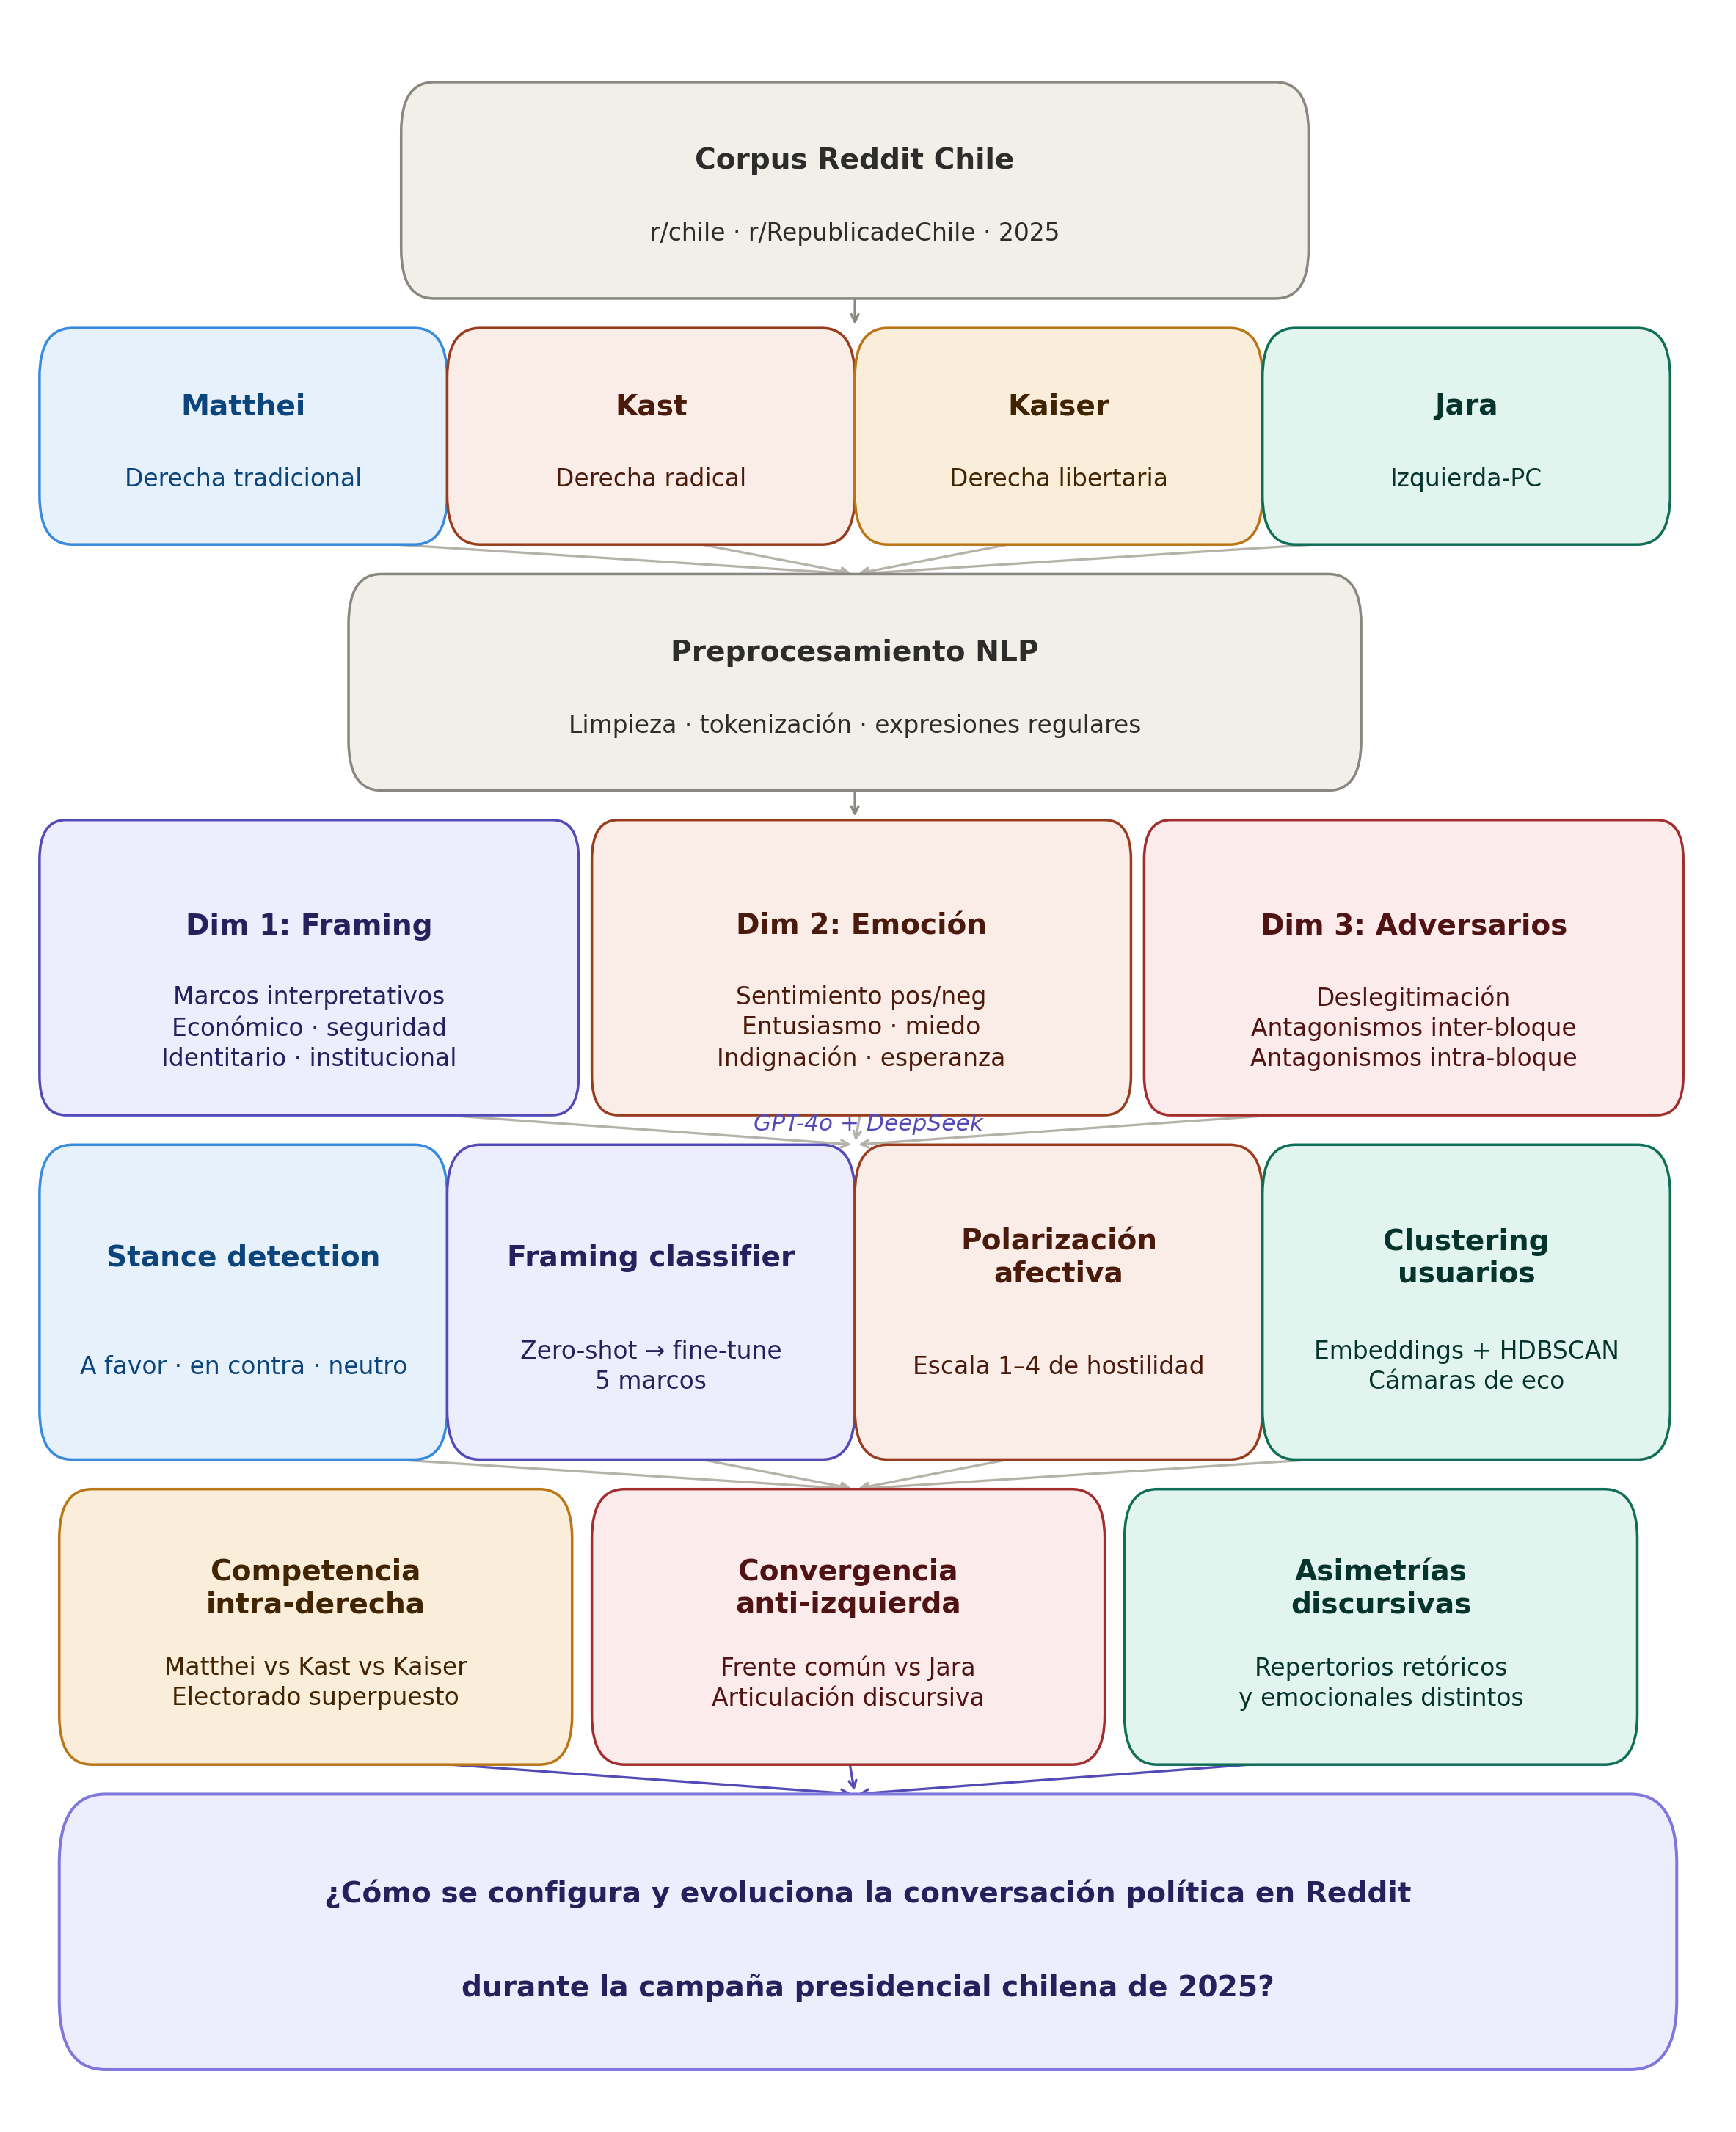
\includegraphics[width=0.9\textwidth,height=\textheight]{fig_thesis/diagrama.png}

}

\caption{\label{fig-pipeline}Pipeline analítico: de la recolección del
corpus a los hallazgos sustantivos.}

\end{figure}%

La Figure~\ref{fig-pipeline} sintetiza el encadenamiento entre corpus,
procesamiento, modelamiento y hallazgos.

\subsection{Arquitectura del
análisis}\label{arquitectura-del-anuxe1lisis}

\textbf{Fase 1: Caracterización del corpus} - Estadísticas descriptivas:
volumen, distribución temporal, participación por subreddit - Mapeo de
actores: frecuencia de mención de cada candidatura - Identificación de
eventos: picos de actividad y su correlación con acontecimientos
políticos

\textbf{Fase 2: Análisis de encuadres} - Modelado de tópicos para
identificar temas estructurantes - Análisis de co-ocurrencias: qué
conceptos aparecen asociados a cada candidatura - Comparación
inter-temporal: evolución de marcos entre primera y segunda vuelta

\textbf{Fase 3: Análisis emocional} - Clasificación de sentimiento
(positivo/negativo/neutro) - Identificación de emociones discretas
cuando es posible - Construcción de ``perfiles emocionales'' por
candidatura

\textbf{Fase 4: Análisis de adversarios} - Identificación de menciones
cruzadas entre candidaturas - Clasificación de valencia: menciones
positivas, negativas, neutras - Mapeo de redes de antagonismo

\textbf{Fase 5: Síntesis e integración} - Triangulación de hallazgos
entre dimensiones - Construcción de narrativa analítica - Identificación
de mecanismos explicativos

\subsection{Originalidad de la
propuesta}\label{originalidad-de-la-propuesta}

La propuesta se distingue de estudios previos en tres aspectos:

\begin{enumerate}
\def\labelenumi{\arabic{enumi}.}
\item
  \textbf{Foco en competencia intra-bloque}: Mientras la mayoría de
  estudios examina la polarización entre izquierda y derecha, esta
  investigación centra la atención en las dinámicas \emph{dentro} del
  campo de las derechas.
\item
  \textbf{Perspectiva procesual}: En lugar de fotografías estáticas, el
  diseño longitudinal permite observar cómo evolucionan las estrategias
  discursivas a lo largo del ciclo electoral.
\item
  \textbf{Reddit como campo}: La plataforma está subexplorada en el
  contexto latinoamericano, y sus características estructurales
  (conversaciones anidadas, votación comunitaria) ofrecen posibilidades
  analíticas distintivas.
\end{enumerate}

\section{Producto mínimo viable (MVP) y objetivos
operacionales}\label{producto-muxednimo-viable-mvp-y-objetivos-operacionales}

\subsection{Definición del MVP}\label{definiciuxf3n-del-mvp}

El \textbf{producto mínimo viable} de esta investigación consiste en:

\begin{quote}
Un análisis sistemático de la conversación política en Reddit sobre las
candidaturas presidenciales chilenas de 2025, que identifique y
caracterice los patrones de encuadre, emoción y construcción de
adversarios de cada corriente ideológica, y que documente su evolución a
lo largo del ciclo electoral (agosto-diciembre 2025).
\end{quote}

\subsection{Objetivos operacionales y
entregables}\label{objetivos-operacionales-y-entregables}

\begin{longtable}[]{@{}
  >{\raggedright\arraybackslash}p{(\columnwidth - 4\tabcolsep) * \real{0.2466}}
  >{\raggedright\arraybackslash}p{(\columnwidth - 4\tabcolsep) * \real{0.2740}}
  >{\raggedright\arraybackslash}p{(\columnwidth - 4\tabcolsep) * \real{0.4795}}@{}}
\caption{Objetivos operacionales, entregables e indicadores de
cumplimiento del MVP.}\label{tbl-objetivos-mvp}\tabularnewline
\toprule\noalign{}
\begin{minipage}[b]{\linewidth}\raggedright
Objetivo
\end{minipage} & \begin{minipage}[b]{\linewidth}\raggedright
Entregable
\end{minipage} & \begin{minipage}[b]{\linewidth}\raggedright
Indicador de cumplimiento
\end{minipage} \\
\midrule\noalign{}
\endfirsthead
\toprule\noalign{}
\begin{minipage}[b]{\linewidth}\raggedright
Objetivo
\end{minipage} & \begin{minipage}[b]{\linewidth}\raggedright
Entregable
\end{minipage} & \begin{minipage}[b]{\linewidth}\raggedright
Indicador de cumplimiento
\end{minipage} \\
\midrule\noalign{}
\endhead
\bottomrule\noalign{}
\endlastfoot
\textbf{O1}: Construir corpus & Base de datos estructurada & ≥1000 posts
y ≥10.000 comentarios con menciones políticas \\
\textbf{O2}: Mapear emociones & Perfiles emocionales por candidatura &
Clasificación de polarización y emociones \\
\textbf{O4}: Analizar adversarios & Red de antagonismos & Matriz de
menciones cruzadas con valencia \\
\textbf{O5}: Documentar evolución & Serie temporal & Análisis por fase
electoral (pre-campaña, campaña, segunda vuelta) \\
\textbf{O6}: Sintetizar hallazgos & Capítulos de resultados & Respuesta
fundamentada a cada pregunta de investigación \\
\end{longtable}

La planificación operativa del estudio se detalla en la
Table~\ref{tbl-objetivos-mvp}.

\subsection{Alcances y limitaciones
anticipadas}\label{alcances-y-limitaciones-anticipadas}

\textbf{Alcances}: - El análisis cubre el debate en dos comunidades de
Reddit, que constituyen los principales espacios de discusión política
chilena en la plataforma. - El período captura fases clave del ciclo
electoral, permitiendo observar dinámicas de cambio. - Las técnicas
empleadas permiten procesar el corpus completo, no solo muestras.

\textbf{Limitaciones}: - Reddit no es representativo del electorado
chileno; los hallazgos refieren al debate en esta plataforma específica,
no a la opinión pública general. - Los usuarios de Reddit tienden a ser
más jóvenes, más masculinos y más politizados que la población general.
- El análisis de sentimiento automatizado tiene márgenes de error,
particularmente con ironía, sarcasmo y jerga local. - La atribución
ideológica de usuarios es inferida a partir de su comportamiento
discursivo, no de autodeclaraciones.

\section{Estrategia de validación}\label{estrategia-de-validaciuxf3n}

\subsection{Validación interna}\label{validaciuxf3n-interna}

\textbf{Triangulación metodológica}: Los hallazgos de cada técnica son
contrastados entre sí. Un patrón se considera robusto cuando emerge
consistentemente de múltiples aproximaciones.

\textbf{Verificación cualitativa}: Los patrones identificados
computacionalmente son verificados mediante lectura de casos. Cuando el
análisis automatizado clasifica un comentario como ``negativo hacia
Matthei'', se revisan ejemplos para confirmar que la clasificación
captura el fenómeno de interés.

\textbf{Sensibilidad paramétrica}: Las técnicas con parámetros
ajustables son ejecutadas con múltiples configuraciones para verificar
que los hallazgos no dependan de decisiones arbitrarias.

\subsection{Validación externa}\label{validaciuxf3n-externa}

\textbf{Triangulación con fuentes externas}: Los patrones temporales
identificados en Reddit son contrastados con el calendario de eventos
políticos documentado en medios de comunicación. La correlación entre
picos de actividad y eventos específicos (debates, declaraciones,
encuestas) proporciona validación externa.

\textbf{Consistencia con literatura}: Los hallazgos son discutidos a la
luz de estudios previos sobre comunicación política digital, derechas
latinoamericanas y polarización. La convergencia con patrones
documentados en otros contextos refuerza la validez; las divergencias
son examinadas como posibles especificidades del caso chileno.

\subsection{Criterios de éxito}\label{criterios-de-uxe9xito}

La investigación se considerará exitosa si:

\begin{enumerate}
\def\labelenumi{\arabic{enumi}.}
\item
  \textbf{Responde las preguntas}: Cada pregunta de investigación recibe
  una respuesta fundamentada empíricamente.
\item
  \textbf{Identifica patrones no triviales}: Los hallazgos van más allá
  de lo que podría inferirse sin análisis sistemático.
\item
  \textbf{Documenta variación}: El análisis captura diferencias
  significativas entre corrientes ideológicas, entre subreddits y entre
  fases electorales.
\item
  \textbf{Genera interpretaciones plausibles}: Los patrones
  identificados son interpretados mediante mecanismos teóricamente
  informados.
\item
  \textbf{Reconoce limitaciones}: El análisis explicita qué puede y qué
  no puede concluirse a partir de los datos disponibles.
\end{enumerate}

\bookmarksetup{startatroot}

\chapter{Marco teórico}\label{marco-teuxf3rico}

\section{Polarización afectiva}\label{polarizaciuxf3n-afectiva}

La polarización afectiva designa el distanciamiento emocional entre
grupos políticos: no solo divergen en posiciones, sino que se desagradan
y se atribuyen mutuamente malas intenciones (Iyengar, 2019). Es
analíticamente distinta de la polarización ideológica --- ambas pueden
variar de manera independiente --- y la evidencia comparada sugiere que
la afectiva ha crecido más rápidamente en democracias contemporáneas
(Boxell, 2022).

Sus principales mecanismos en entornos digitales incluyen la exposición
selectiva amplificada por algoritmos, la mayor visibilidad de voces
extremas, la reducción de costos de expresión hostil y las dinámicas de
señalización grupal recompensadas con métricas de aprobación (Brady,
2017; Settle, 2018). Las consecuencias para la democracia son
significativas: erosión de la confianza institucional, resistencia al
compromiso y tolerancia a la transgresión normativa cuando proviene del
propio bando (Graham, 2020).

\section{Construcción de adversarios y frontera
política}\label{construcciuxf3n-de-adversarios-y-frontera-poluxedtica}

Las identidades colectivas no son esencias preexistentes: emergen a
través de la diferenciación. Todo ``nosotros'' se constituye en relación
con un ``ellos'' (Laclau, 1985). Mouffe (2005) distingue antagonismo ---
relación entre enemigos sin espacio común --- de agonismo --- relación
entre adversarios que comparten el marco democrático. Esta distinción
permite preguntar si los actores construyen a sus oponentes como
participantes legítimos o como amenazas existenciales.

Las estrategias de deslegitimación incluyen asociación negativa,
atribución de intenciones ocultas, ridiculización, esencialización y
construcción de amenaza. Para esta investigación resulta crucial
distinguir entre fronteras inter-bloque (izquierda vs.~derecha) y
fronteras intra-bloque (entre corrientes de derecha), que generan
tensiones estratégicas entre diferenciación y convergencia.

\section{Encuadre y emociones en el discurso
político}\label{encuadre-y-emociones-en-el-discurso-poluxedtico}

El encuadre consiste en seleccionar aspectos de la realidad y hacerlos
prominentes para promover una definición del problema, una
interpretación causal y una evaluación moral (Entman, 1993). Se
distinguen marcos genéricos --- conflicto, consecuencias económicas,
atribución de responsabilidad, moralidad --- y marcos específicos
propios de cada controversia (Semetko, 2000). Para campañas electorales
resulta útil añadir la distinción entre marcos diagnósticos (¿cuál es el
problema?), pronósticos (¿qué debe hacerse?) y motivacionales (¿qué está
en juego?).

Las emociones, por su parte, no son ruido que distorsiona el juicio
racional: son componentes constitutivos de la cognición y la acción
política (Marcus, 2000). El concepto de repertorio afectivo --- la
configuración característica de emociones movilizadas por un actor, su
combinación y los objetos hacia los que se dirigen --- resulta más
operativo que el registro de emociones aisladas (Jasper, 2011). La
indignación moral merece atención especial: combina valencia negativa
con alta activación y orientación a la acción, se difunde más que otras
emociones y genera bajo costo de expresión con recompensas sociales
inmediatas (Crockett, 2017).

Encuadre y emoción se articulan en el análisis como dimensiones
complementarias: el marco establece \emph{de qué} se habla, la emoción
determina \emph{con qué intensidad y valencia} se habla. Su combinación
--- por ejemplo, un marco de conflicto acoplado con desprecio versus un
marco diagnóstico acoplado con indignación --- constituye lo que esta
tesis denomina \emph{configuración discursiva}, unidad de análisis
central en los capítulos de resultados.

\section{Derechas contemporáneas en
Chile}\label{derechas-contemporuxe1neas-en-chile}

La coexistencia de múltiples corrientes de derecha en Chile genera
dinámicas de competencia intra-bloque que constituyen un laboratorio
analítico de particular valor. Estas corrientes difieren no solo
ideológicamente sino en sus estrategias comunicativas: la derecha
tradicional emplea un registro institucional y moderado; la radical
populista moviliza agravios y retórica de confrontación; la libertaria
combina argumentos económicos con estilos provocadores y referencias a
subculturas digitales (Norris, 2019). En el contexto de la campaña
presidencial de 2025, los candidatos Matthei, Kast, Kaiser y Jara
representan posiciones diferenciadas dentro de este espectro, con
estrategias de diferenciación interna que conviven con presiones de
convergencia frente al adversario común de izquierda.

\section{Reddit como espacio de polarización
política}\label{reddit-como-espacio-de-polarizaciuxf3n-poluxedtica}

Reddit se estructura en torno a comunidades temáticas (subreddits) antes
que en redes de relaciones personales, lo que privilegia el debate
sustantivo sobre la identidad individual. Sus comentarios anidados
permiten seguir el desarrollo de argumentos y contraargumentos; el
sistema de votación (karma) ofrece un indicador de resonancia
comunitaria; y la persistencia temporal del contenido habilita el
análisis longitudinal (Proferes, 2021).

Estas propiedades hacen de Reddit un espacio particularmente adecuado
para estudiar la polarización afectiva por tres razones. Primero, el
pseudonimato reduce los costos de expresión hostil en comparación con
plataformas donde la identidad real es visible, lo que puede amplificar
la intensidad del discurso adversarial. Segundo, la estructura anidada
de conversación permite observar el \emph{framing} como proceso: los
marcos son propuestos, contestados y reformulados en tiempo real, a
diferencia de plataformas de flujo lineal como X/Twitter (Meraz, 2013).
Tercero, la coexistencia de comunidades con culturas discursivas
contrastantes dentro de un mismo tema político permite la comparación
controlada.

En el contexto chileno, r/chile (generalista, tendencia
centro-izquierda) y r/RepublicadeChile (surgida como escisión, mayor
tolerancia a discursos confrontacionales) constituyen un caso
comparativo natural. Ambas comunidades procesan las mismas controversias
electorales, pero con normas de moderación, composición ideológica y
umbrales de hostilidad diferenciados. Esta variación permite examinar si
los patrones de polarización observados responden a la estructura del
debate político o a la cultura discursiva específica de cada comunidad.

No obstante, Reddit presenta limitaciones conocidas como corpus de
investigación: sesgo demográfico hacia usuarios jóvenes, masculinos y
con mayor nivel educativo; imposibilidad de verificar identidades
reales; y ausencia de representatividad respecto de la opinión pública
general (Zimmer, 2017). Estas limitaciones se discuten en el capítulo de
conclusiones como acotaciones del alcance interpretativo de los
hallazgos.

\section{Modelo analítico
integrado}\label{modelo-analuxedtico-integrado}

El modelo integrado de esta tesis articula las dimensiones anteriores en
una secuencia analítica orientada por la pregunta central: cómo se
reconfigura el antagonismo político en la conversación digital de
derechas. La polarización afectiva opera como fenómeno a explicar; la
construcción de adversarios y la frontera política como mecanismo
central; el encuadre y las emociones como dimensiones observables del
discurso; y Reddit como espacio empírico donde estas dinámicas se
despliegan. Los capítulos de modelado e interpretación traducen este
esquema en variables operacionales y resultados cuantificables.

\bookmarksetup{startatroot}

\chapter{Diseño metodológico}\label{diseuxf1o-metodoluxf3gico}

\section{Diseño de investigación}\label{diseuxf1o-de-investigaciuxf3n}

Esta investigación adopta un diseño \textbf{l}ongitudinal observacional
basado en datos digitales generados por usuarios (\emph{user-generated
content}). El carácter longitudinal permite capturar la evolución del
debate político a lo largo del ciclo electoral, identificando
tendencias, puntos de inflexión y dinámicas de cambio. El carácter
observacional preserva las propiedades naturales de la interacción en
las plataformas estudiadas, sin intervención experimental.

Metodológicamente, la investigación se inscribe en la \textbf{ciencia
social computacional} (Lazer 2009; Salganik 2019): integra técnicas de
procesamiento de datos a gran escala con marcos teóricos y preguntas
sustantivas de las ciencias sociales. El diseño combina componentes
\textbf{descriptivos} ---caracterizar la conversación política en Reddit
durante el período estudiado--- con componentes \textbf{explicativos},
orientados a identificar los factores y mecanismos que dan cuenta de los
patrones observados.

\section{Reddit como plataforma de
análisis}\label{reddit-como-plataforma-de-anuxe1lisis}

Reddit es una plataforma de agregación de contenido y discusión
organizada en comunidades temáticas denominadas \emph{subreddits}, cada
una con sus propias normas, moderadores y cultura discursiva. A
diferencia de plataformas organizadas en torno a redes de seguidores o
amistades, Reddit estructura la participación en torno a intereses y
temas compartidos, lo que favorece conversaciones más extensas y
argumentadas que en otros entornos digitales.

Su arquitectura de \textbf{comentarios anidados} (\emph{threaded
discussions}) permite seguir el desarrollo de argumentos y
contraargumentos en múltiples niveles, haciendo visible la estructura
deliberativa del debate. Los usuarios operan bajo seudónimos no
vinculados a su identidad real, lo que puede facilitar la expresión de
posiciones polémicas. Las comunidades son autogobernadas: cada subreddit
define sus propias reglas de participación, generando culturas
discursivas distintivas que hacen de la comparación entre comunidades un
ejercicio analíticamente valioso.

En el contexto chileno, dos subreddits concentran la discusión política
nacional:

\begin{itemize}
\tightlist
\item
  \textbf{r/chile}: Comunidad generalista sobre temas chilenos, con
  mayor volumen de usuarios y diversidad temática. Ha tendido
  históricamente hacia posiciones de centro-izquierda, aunque con
  presencia de voces diversas.
\item
  \textbf{r/RepublicadeChile}: Comunidad surgida como escisión de
  r/chile, con políticas de moderación más permisivas y una composición
  ideológica tendiente a la derecha. Tolera discursos más
  confrontacionales y concentra usuarios críticos de la moderación de
  r/chile.
\end{itemize}

Esta dualidad constituye un caso comparativo de valor: permite examinar
cómo una misma controversia política es procesada de manera diferenciada
según la cultura discursiva de la comunidad.

\section{Recolección de datos mediante la API de
Reddit}\label{recolecciuxf3n-de-datos-mediante-la-api-de-reddit}

\subsection{Procedimiento técnico}\label{procedimiento-tuxe9cnico}

Los datos fueron extraídos mediante la API pública de Reddit utilizando
la librería PRAW (\emph{Python Reddit API Wrapper}). Esta aproximación
---distinta del \emph{web scraping} no autorizado--- accede de forma
estructurada a contenido público respetando los límites de uso
establecidos por la plataforma y garantizando la trazabilidad y
reproducibilidad del proceso.

\subsection{Período de recolección y fases del ciclo
electoral}\label{peruxedodo-de-recolecciuxf3n-y-fases-del-ciclo-electoral}

La recolección abarcó \textbf{cinco meses}, del \textbf{1 de agosto al
31 de diciembre de 2025}, cubriendo las siguientes fases del ciclo
electoral:

\begin{longtable}[]{@{}
  >{\raggedright\arraybackslash}p{(\columnwidth - 2\tabcolsep) * \real{0.2373}}
  >{\raggedright\arraybackslash}p{(\columnwidth - 2\tabcolsep) * \real{0.7627}}@{}}
\toprule\noalign{}
\begin{minipage}[b]{\linewidth}\raggedright
Período
\end{minipage} & \begin{minipage}[b]{\linewidth}\raggedright
Fase electoral
\end{minipage} \\
\midrule\noalign{}
\endhead
\bottomrule\noalign{}
\endlastfoot
Agosto -- octubre 2025 & Emergencia de candidaturas, posicionamiento
inicial, primeras definiciones programáticas \\
Noviembre -- diciembre 2025 & Escalamiento de campaña, consolidación
electoral, estructuración del debate público \\
\end{longtable}

\subsection{Estrategia de extracción
incremental}\label{estrategia-de-extracciuxf3n-incremental}

El proceso fue \textbf{incremental y acumulativo}, ejecutado en
múltiples iteraciones que: (1) recuperaban los posts más recientes de
cada subreddit (250--1.000 posts por ejecución); (2) descargaban el
árbol completo de comentarios para capturar todos los niveles de
anidación; (3) integraban nuevos datos con extracciones previas en
archivos Parquet; y (4) eliminaban duplicados mediante el identificador
único nativo de Reddit (\texttt{post\_id}), que garantiza unicidad por
diseño de la plataforma.

\subsection{Contenido extraído y filtrado
temático}\label{contenido-extrauxeddo-y-filtrado-temuxe1tico}

Para cada publicación dentro del rango temporal se extrajeron dos
niveles:

\textbf{Posts}: título, cuerpo (\emph{selftext}), autor, fecha,
puntuación, número de comentarios y flair temático.

\textbf{Comentarios}: cuerpo del comentario, autor, fecha, puntuación e
identificador del comentario al que responde.

El filtrado temático se realizó mediante \textbf{expresiones regulares}
que detectan menciones de las cuatro candidaturas de interés, manejando
variaciones ortográficas (acentuación, nombres completos vs.~apellidos,
apodos y errores tipográficos frecuentes):

\begin{longtable}[]{@{}
  >{\raggedright\arraybackslash}p{(\columnwidth - 4\tabcolsep) * \real{0.2235}}
  >{\raggedright\arraybackslash}p{(\columnwidth - 4\tabcolsep) * \real{0.3529}}
  >{\raggedright\arraybackslash}p{(\columnwidth - 4\tabcolsep) * \real{0.4235}}@{}}
\caption{Candidaturas objetivo y patrones de
detección.}\label{tbl-candidaturas}\tabularnewline
\toprule\noalign{}
\begin{minipage}[b]{\linewidth}\raggedright
Candidatura
\end{minipage} & \begin{minipage}[b]{\linewidth}\raggedright
Corriente ideológica
\end{minipage} & \begin{minipage}[b]{\linewidth}\raggedright
Patrones de búsqueda
\end{minipage} \\
\midrule\noalign{}
\endfirsthead
\toprule\noalign{}
\begin{minipage}[b]{\linewidth}\raggedright
Candidatura
\end{minipage} & \begin{minipage}[b]{\linewidth}\raggedright
Corriente ideológica
\end{minipage} & \begin{minipage}[b]{\linewidth}\raggedright
Patrones de búsqueda
\end{minipage} \\
\midrule\noalign{}
\endhead
\bottomrule\noalign{}
\endlastfoot
Evelyn Matthei & Derecha tradicional & \texttt{matthei}, \texttt{matei},
\texttt{evelyn} \\
José Antonio Kast & Derecha radical-conservadora & \texttt{kast},
\texttt{jose\ antonio\ kast}, \texttt{jak} \\
Johannes Kaiser & Derecha libertaria & \texttt{kaiser},
\texttt{johannes}, \texttt{jkaiser} \\
Jeannette Jara & Izquierda-PC & \texttt{jara}, \texttt{jeannette},
\texttt{jeanette} \\
\end{longtable}

Esta selección permite analizar tanto la \textbf{competencia
intra-derecha} entre tres corrientes como la \textbf{convergencia
discursiva} frente al adversario ideológico común (ver
Table~\ref{tbl-candidaturas}).

\section{Consideraciones éticas}\label{consideraciones-uxe9ticas}

La investigación se rige por principios establecidos para la
investigación con datos digitales (Salganik 2019; Zimmer 2017):

\textbf{Datos públicos}: Todo el contenido recolectado proviene de
espacios públicos de Reddit. No se accedió a mensajes privados ni a
información restringida.

\textbf{Privacidad}: El análisis no reporta identificadores individuales
ni busca vincular cuentas con identidades reales. Los ejemplos citados
son anonimizados cuando resulta pertinente.

\textbf{No intervención}: La investigación no actúa sobre las
comunidades estudiadas ni expone a sus miembros a riesgos adicionales;
el foco es el análisis de dinámicas colectivas.

\textbf{Reproducibilidad}: Los scripts de recolección y procesamiento
están documentados para permitir la replicación del estudio respetando
los términos de uso de la API.

\section{Técnicas de Análisis}\label{tuxe9cnicas-de-anuxe1lisis}

El estudio combina \textbf{modelos de lenguaje (GPT-4o y DeepSeek)} con
\textbf{validación humana sistemática} para analizar discursos políticos
en Reddit. Las clasificaciones automáticas (sentimiento, emociones,
marcos y estrategias) se realizan mediante prompts estructurados y luego
se \textbf{validan con codificación manual} usando métricas de acuerdo
(Cohen's κ) antes de escalar al corpus completo.

Se analizan cuatro dimensiones principales:

\begin{itemize}
\item
  \textbf{Sentimiento y emociones} (polaridad, intensidad y emoción
  predominante)
\item
  \textbf{Marcos interpretativos} (económico, seguridad, identitario,
  institucional, medioambiental)
\item
  \textbf{Interacciones} (redes de respuesta entre usuarios para
  detectar comunidades y polarización)
\item
  \textbf{Evolución temporal} (cambios en tono, temas y volumen a lo
  largo del tiempo)
\end{itemize}

El pipeline incluye técnicas de \textbf{procesamiento de texto (TF-IDF,
bigramas)}, codificación de variables y modelos supervisados como
\textbf{Regresión Logística, SVM, Random Forest y Gradient Boosting},
evaluados con validación cruzada. También se aplican métodos de
\textbf{reducción de dimensionalidad (SVD y PCA)} para visualización.

Los desacuerdos entre modelos se utilizan como señal de ambigüedad y se
resuelven mediante revisión humana o criterios adicionales. El corpus
final incluye publicaciones y comentarios de r/chile y
r/RepublicadeChile durante todo el ciclo electoral, permitiendo análisis
\textbf{longitudinales, relacionales y discursivos integrados}

\begin{figure}[H]

\centering{

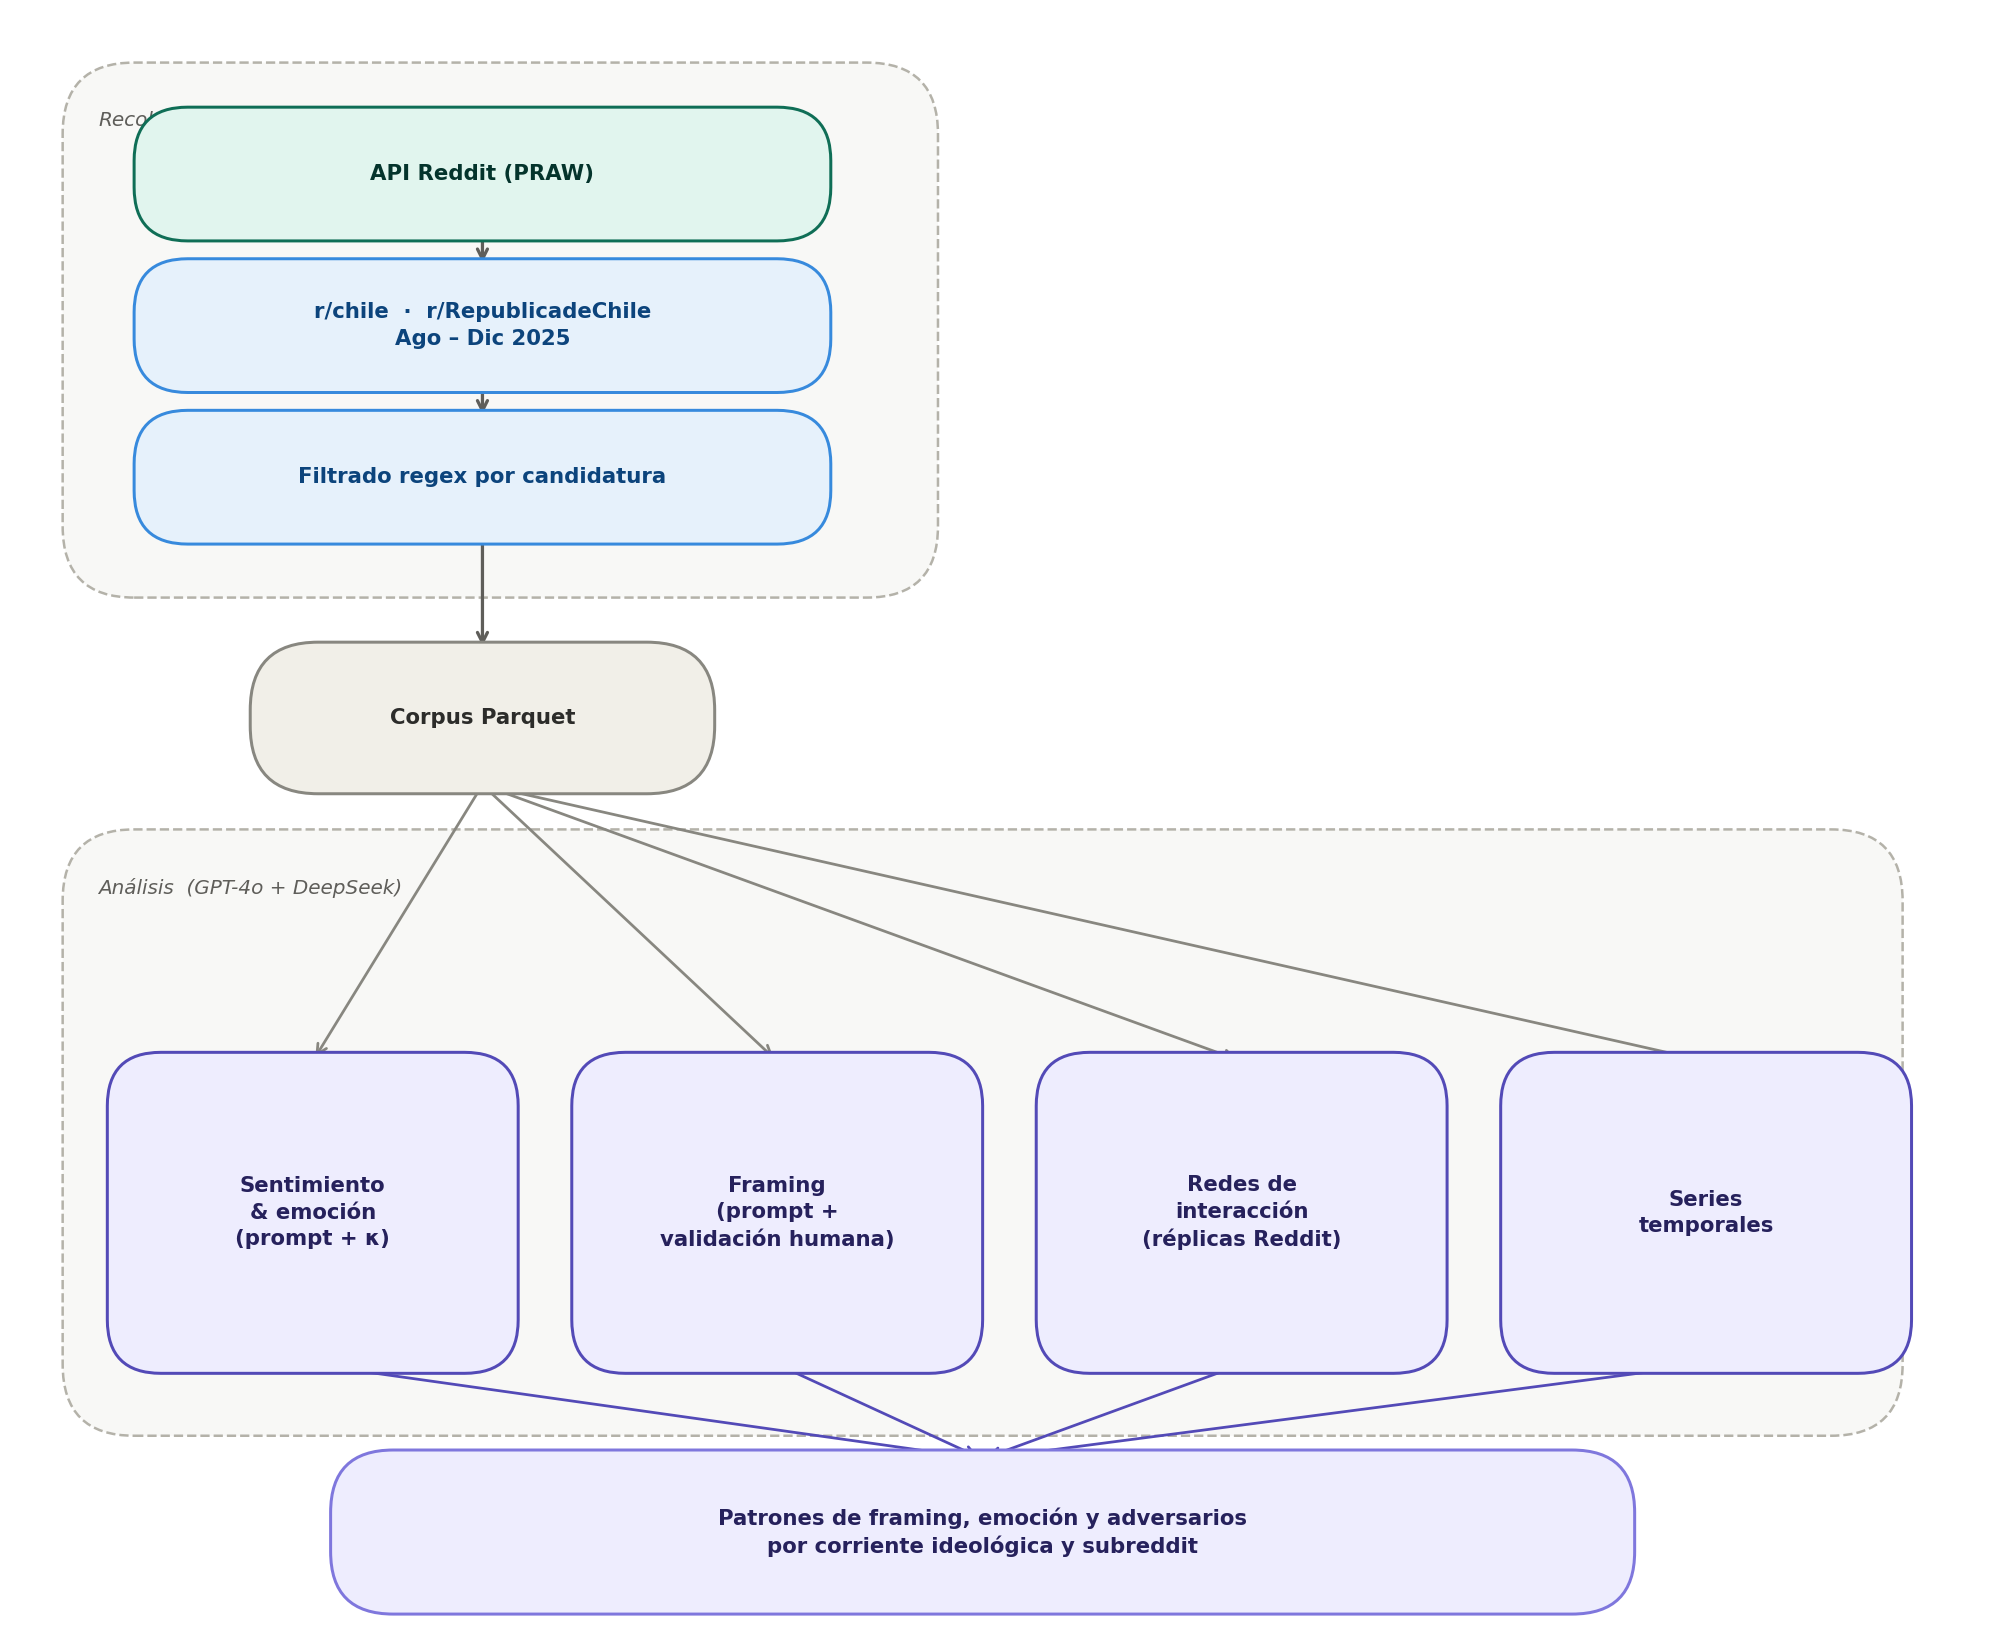
\includegraphics[width=0.9\textwidth,height=\textheight]{fig_thesis/pipeline_corpus.png}

}

\caption{\label{fig-pipeline-datos}Flujo de recolección y procesamiento
del corpus.}

\end{figure}%

\bookmarksetup{startatroot}

\chapter{Depuración de Datos}\label{depuraciuxf3n-de-datos}

\section{Depuración y preprocesamiento del
corpus}\label{depuraciuxf3n-y-preprocesamiento-del-corpus}

Una vez constituido el corpus filtrado temáticamente, se aplicó una
etapa de depuración orientada a garantizar la calidad analítica de los
datos. Esta etapa distingue entre dos tipos de decisiones: las que
afectan a unidades de observación ---posts y comentarios que son
excluidos del análisis--- y las que afectan al contenido textual
---transformaciones aplicadas al texto para mejorar su
procesabilidad---.

\section{Descripción general del
corpus}\label{descripciuxf3n-general-del-corpus}

El corpus previo a la depuración comprende \textbf{163.695 comentarios}
distribuidos en \textbf{4.105 posts únicos}, publicados entre 05 de
August de 2025 y 22 de January de 2026. Participaron \textbf{9.845
autores únicos} en los comentarios y \textbf{1.106 autores únicos} en
los posts. La Table~\ref{tbl-general} resume las estadísticas generales
del corpus en esta etapa inicial.

\begin{longtable}[t]{lr}

\caption{\label{tbl-general}Estadísticas generales del corpus.}

\tabularnewline

\toprule
Indicador & Valor\\
\midrule
\cellcolor{gray!10}{Comentarios totales} & \cellcolor{gray!10}{163.695}\\
Posts únicos & 4.105\\
\cellcolor{gray!10}{Autores de posts} & \cellcolor{gray!10}{1.106}\\
Autores de comentarios & 9.845\\
\cellcolor{gray!10}{Posts sin cuerpo textual (solo título)} & \cellcolor{gray!10}{99.434 (60.7\%)}\\
\bottomrule

\end{longtable}

Destaca que una proporción elevada de posts carece de cuerpo textual
(\texttt{post\_selftext\ =\ NA}), lo que implica que la detección de
candidaturas mediante expresiones regulares recae principalmente sobre
los títulos de los posts y el cuerpo de los comentarios. Este patrón es
consistente con la cultura de publicación de Reddit, donde los posts de
tipo \emph{link} o imagen no incluyen texto propio.

\begin{longtable}[t]{lrr}

\caption{\label{tbl-menciones}Frecuencia de menciones por candidatura.}

\tabularnewline

\toprule
Candidatura & Menciones & \% del corpus\\
\midrule
\cellcolor{gray!10}{José A. Kast} & \cellcolor{gray!10}{102.759} & \cellcolor{gray!10}{62.8\%}\\
J. Jara & 63.602 & 38.9\%\\
\cellcolor{gray!10}{J. Kaiser} & \cellcolor{gray!10}{26.521} & \cellcolor{gray!10}{16.2\%}\\
E. Matthei & 16.358 & 10.0\%\\
\bottomrule
\multicolumn{3}{l}{\rule{0pt}{1em}\textit{Nota:} Un comentario puede mencionar a más de un candidato; los porcentajes no suman 100\%.}\\

\end{longtable}

\section{Criterios de exclusión de
unidades}\label{criterios-de-exclusiuxf3n-de-unidades}

Se aplicaron dos criterios de exclusión secuenciales:

\textbf{Contenido automático y bots.} Se identificaron y excluyeron
cuentas con comportamiento consistente con automatización,
operacionalizadas como usuarios que publican más de cincuenta
comentarios en un mismo día de forma sostenida, o cuyos nombres de
usuario coinciden con patrones conocidos de bots en subreddits chilenos
(\texttt{AutoModerator}, \texttt{RemindMeBot}). La exclusión de este
contenido reduce el ruido no-humano en el análisis de sentimiento y en
la construcción de redes de interacción.

\textbf{Comentarios excesivamente cortos.} Los comentarios con menos de
tres tokens tras la normalización (típicamente reacciones monosilábicas,
interjecciones o emojis aislados) aportan información insuficiente para
la clasificación de marcos interpretativos o emociones y fueron
excluidos del análisis textual.

\section{Normalización textual}\label{normalizaciuxf3n-textual}

El texto de posts y comentarios fue sometido a una normalización previa
a cualquier clasificación automatizada. Las transformaciones se
aplicaron en el siguiente orden:

\textbf{Eliminación de elementos no textuales.} URLs, menciones de
usuario (patrones \texttt{u/nombre}), referencias a subreddits
(\texttt{r/nombre}) y secuencias de formato Markdown (asteriscos,
almohadillas, corchetes) fueron eliminadas mediante expresiones
regulares, dado que no aportan contenido semántico al análisis
discursivo.

\textbf{Normalización de espacios y puntuación.} Secuencias de espacios
múltiples, saltos de línea redundantes y puntuación repetida fueron
colapsadas a su forma canónica mediante \texttt{str\_squish()}.

\textbf{Conservación de tildes y caracteres del español.} No se aplicó
eliminación de tildes ni de la letra ñ, dado que su presencia es
relevante para la correcta tokenización del español chileno.

\textbf{No aplicación de \emph{stopwords} ni lematización en esta fase.}
Estas transformaciones más agresivas se reservan para las técnicas que
específicamente las requieren y no se aplican al texto enviado a los
modelos de lenguaje para clasificación de sentimiento y marcos
interpretativos, donde el contexto completo mejora el desempeño del
modelo.

\bookmarksetup{startatroot}

\chapter{Exploración de Datos}\label{exploraciuxf3n-de-datos}

\section{Volumen de comentarios por
candidato}\label{volumen-de-comentarios-por-candidato}

\begin{figure}[H]

\centering{

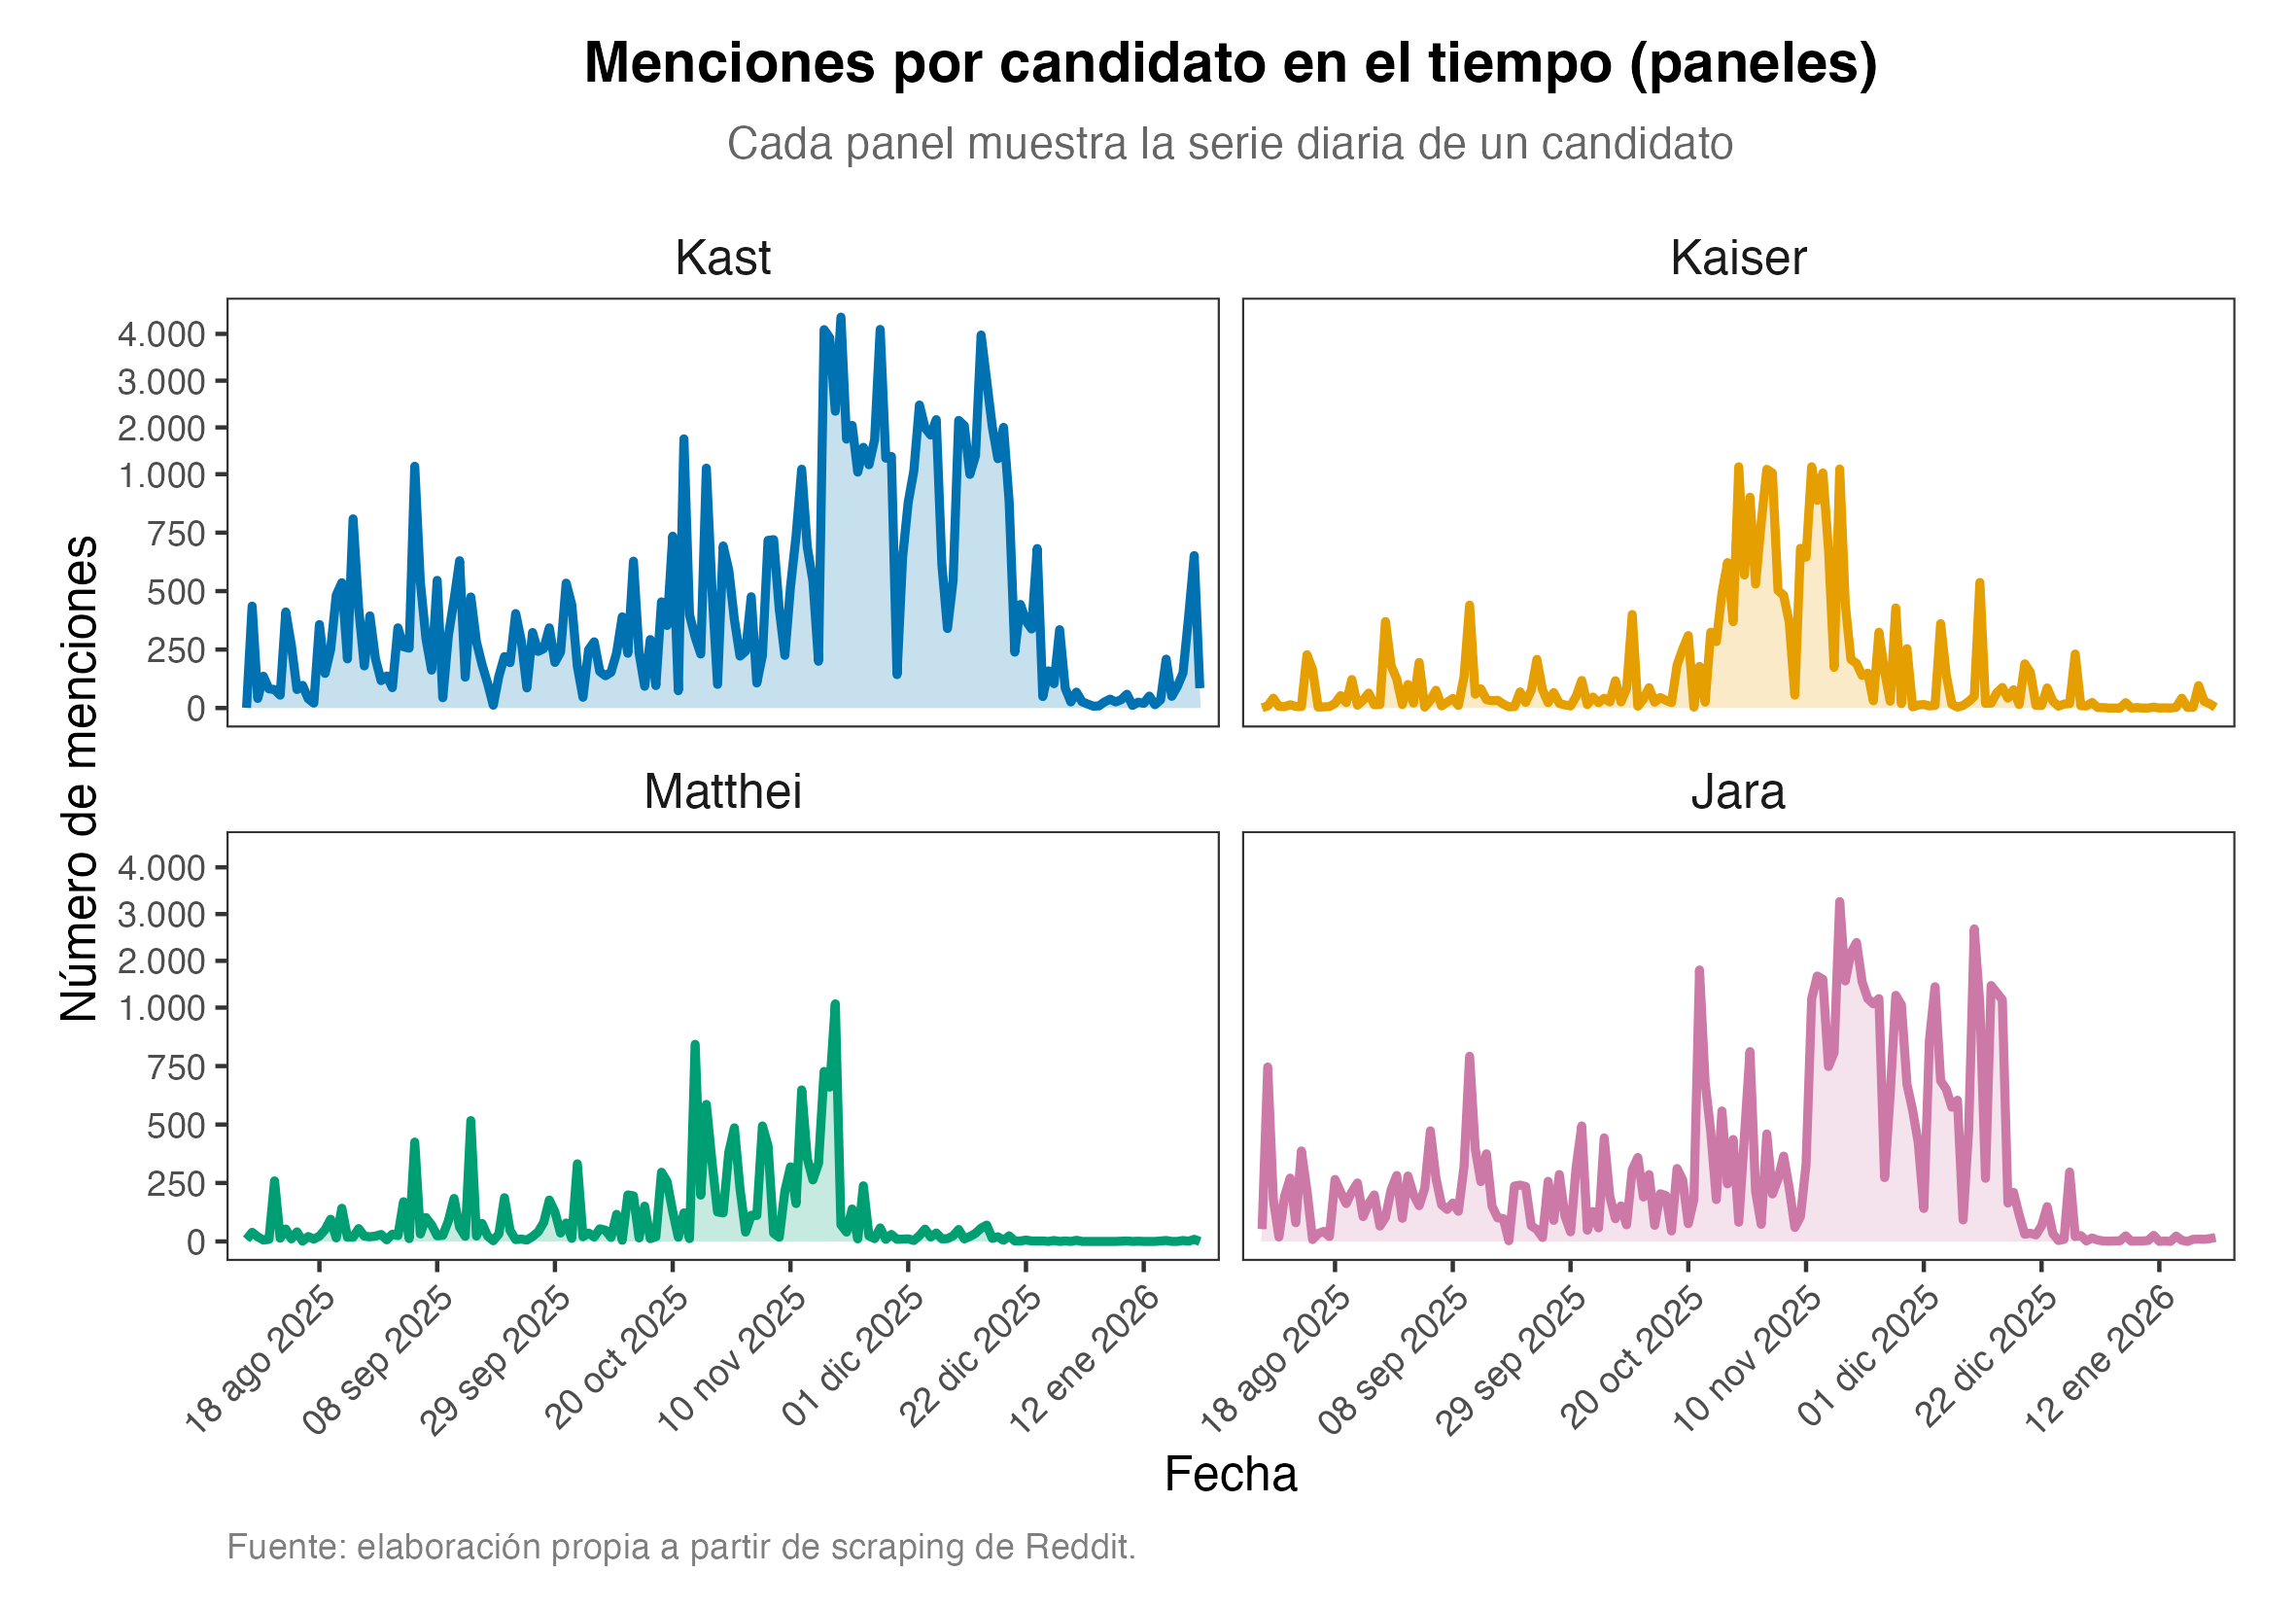
\includegraphics[width=0.92\textwidth,height=\textheight]{fig_thesis/fig_count_facet_candidatos.png}

}

\caption{\label{fig-count-facet-cand}Conteos de comentarios por
candidato (facetas).}

\end{figure}%

La Figure~\ref{fig-count-facet-cand} revela una asimetría marcada en la
atención discursiva. Kast concentra el mayor volumen de menciones
durante todo el período (62.8\% del corpus), seguido por Jara (38.9\%),
con una brecha considerable respecto de Kaiser (16.2\%) y Matthei
(10.0\%). El volumen de menciones de Jara se incrementa hacia el final
del ciclo, coincidiendo con su paso a segunda vuelta, mientras que
Kaiser y Matthei disminuyen tras quedar fuera de la competencia. Esta
distribución desbalanceada implica que los indicadores agregados de
polarización estarán dominados por los comentarios dirigidos a Kast y
Jara, lo que se tiene en cuenta en el diseño del modelado.

\section{Estrategia discursiva y frontera
política}\label{estrategia-discursiva-y-frontera-poluxedtica}

\begin{figure}[H]

\centering{

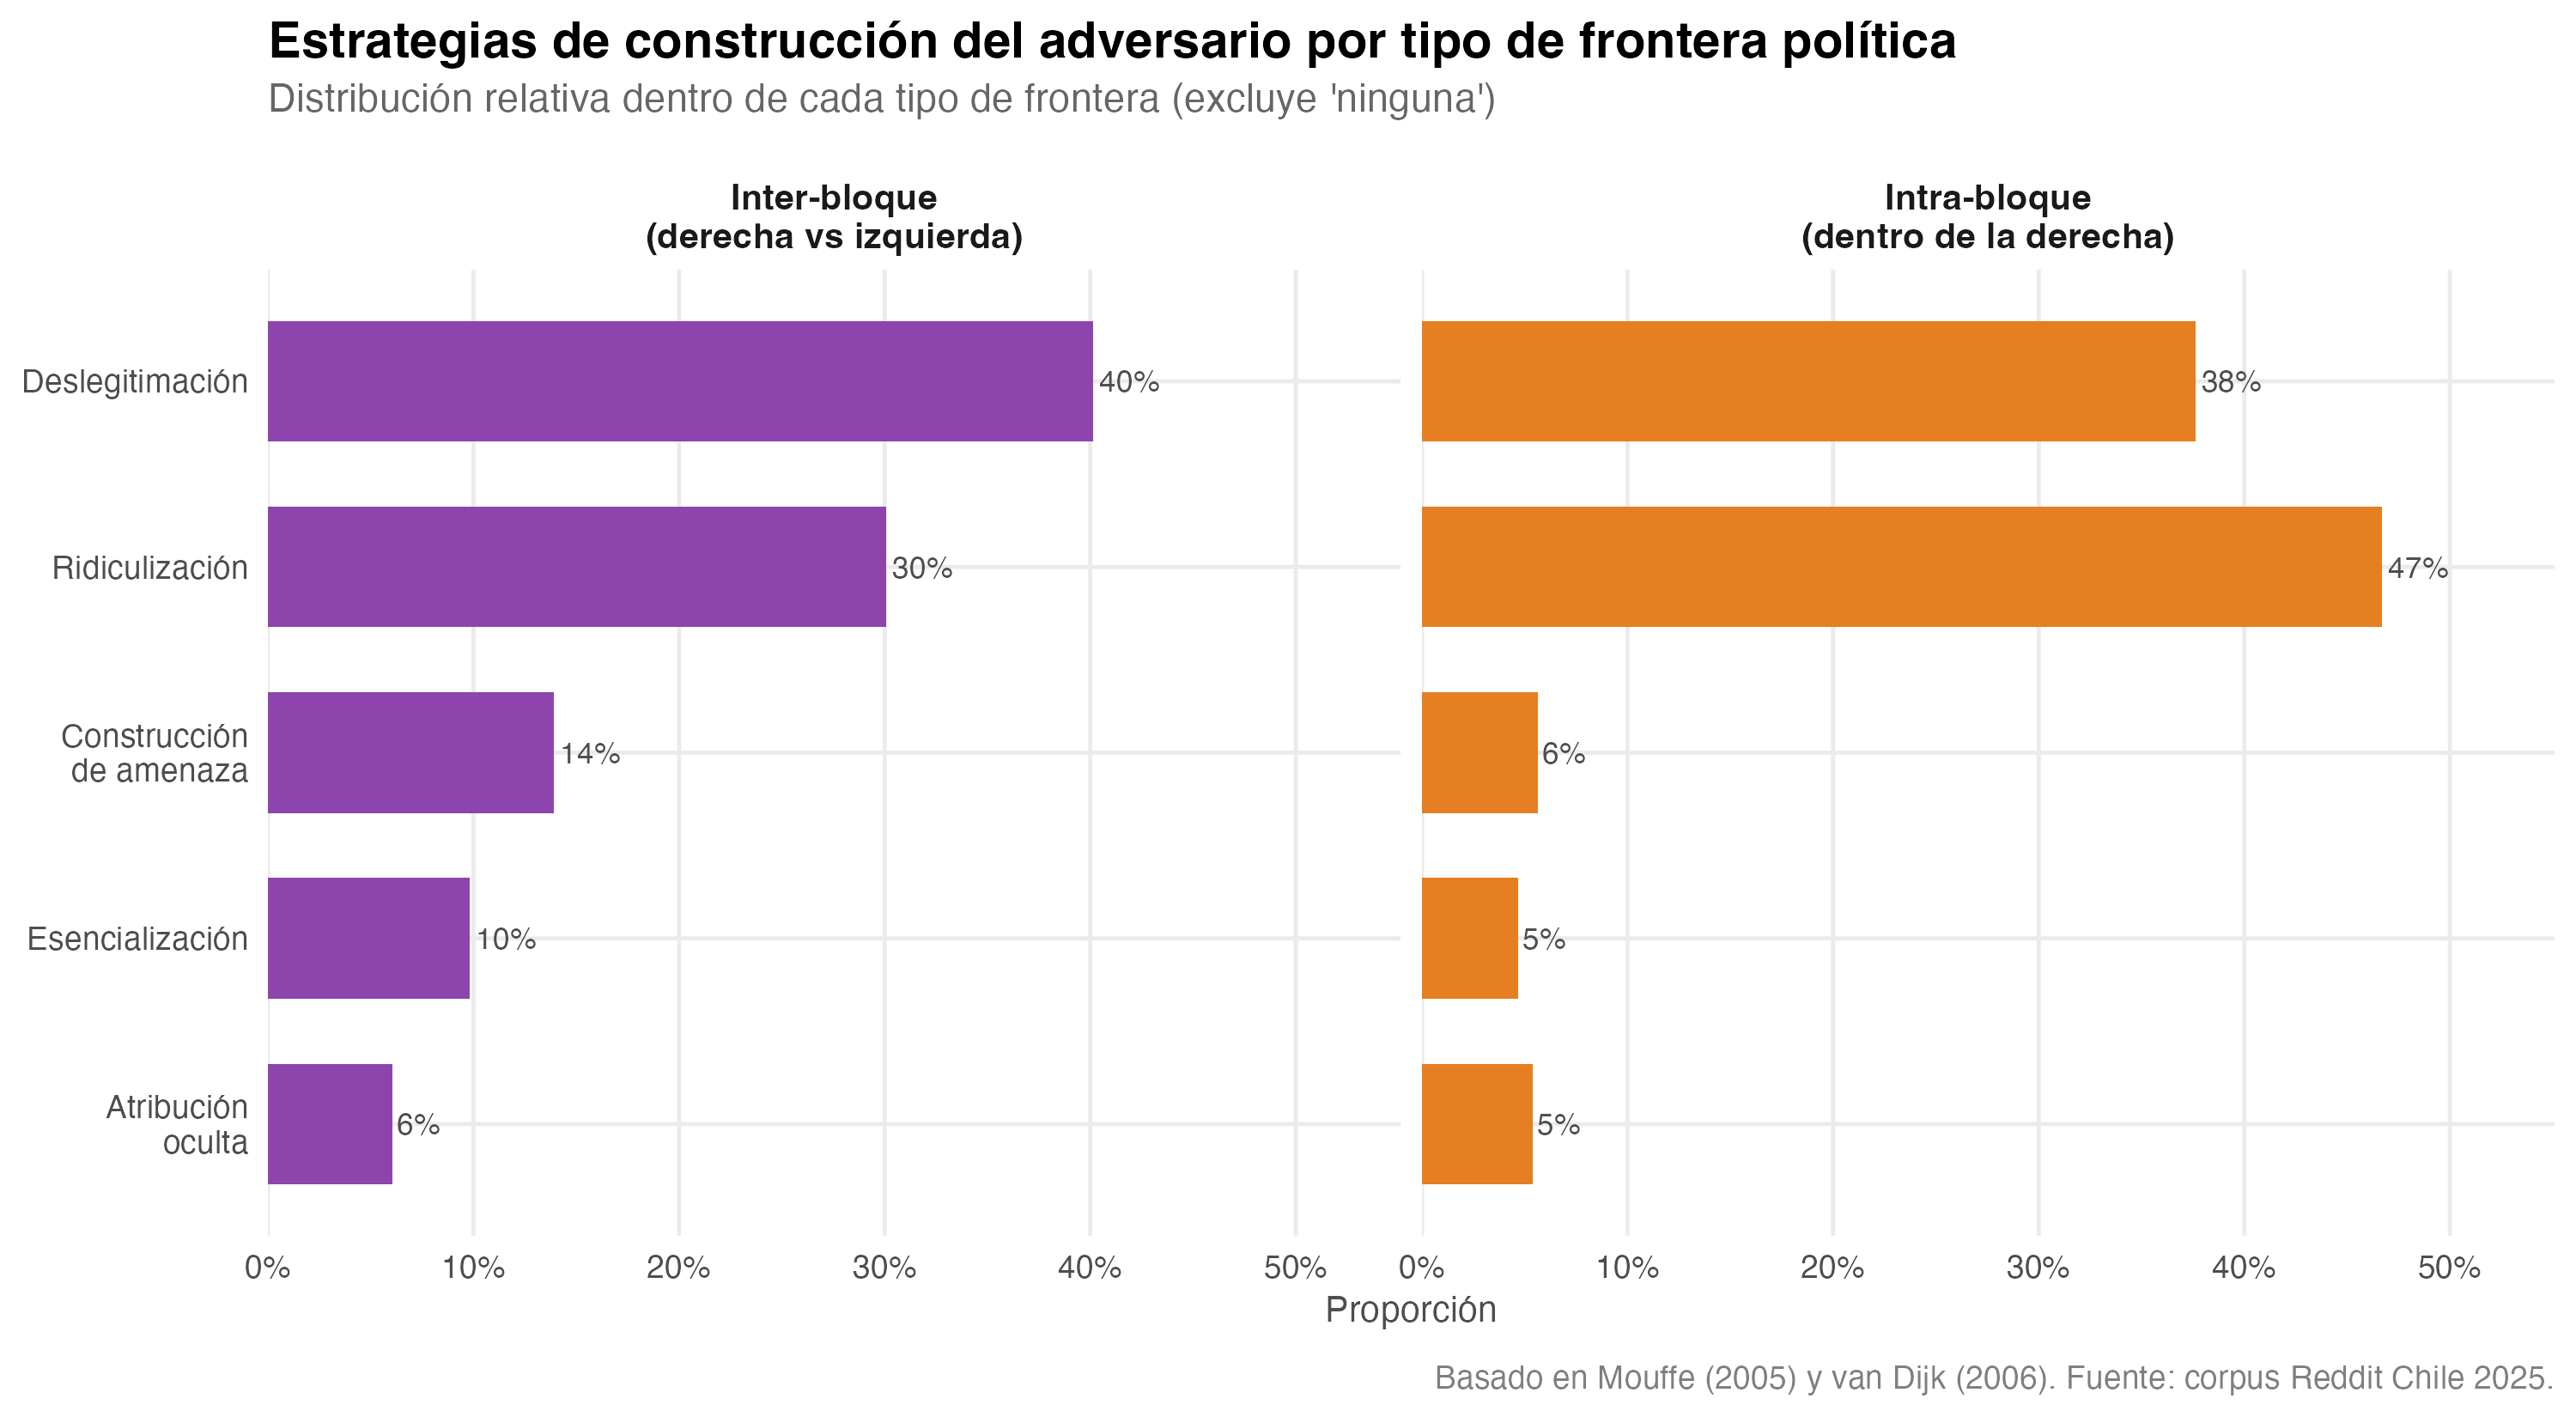
\includegraphics[width=1\textwidth,height=\textheight]{fig_thesis/fig4_estrategia_frontera.png}

}

\caption{\label{fig-explor-estrategia-frontera}Estrategia discursiva y
frontera política por candidato (facetas).}

\end{figure}%

La Figure~\ref{fig-explor-estrategia-frontera} muestra la distribución
relativa de estrategias de construcción del adversario según tipo de
frontera política, separada por candidato. La deslegitimación y la
ridiculización son las estrategias dominantes en todos los candidatos,
pero su distribución entre fronteras varía: la confrontación
inter-bloque (derecha vs.~izquierda) concentra proporcionalmente más
estrategias de amenaza y esencialización, mientras que la disputa
intra-bloque (dentro de la derecha) se canaliza más a través de la
ridiculización. Esta diferenciación preliminar sugiere que la hostilidad
no opera como un fenómeno unitario --- una hipótesis que el capítulo 7
formaliza estadísticamente.

\section{Densidad de polarización por
candidato}\label{densidad-de-polarizaciuxf3n-por-candidato}

\begin{figure}[H]

\centering{

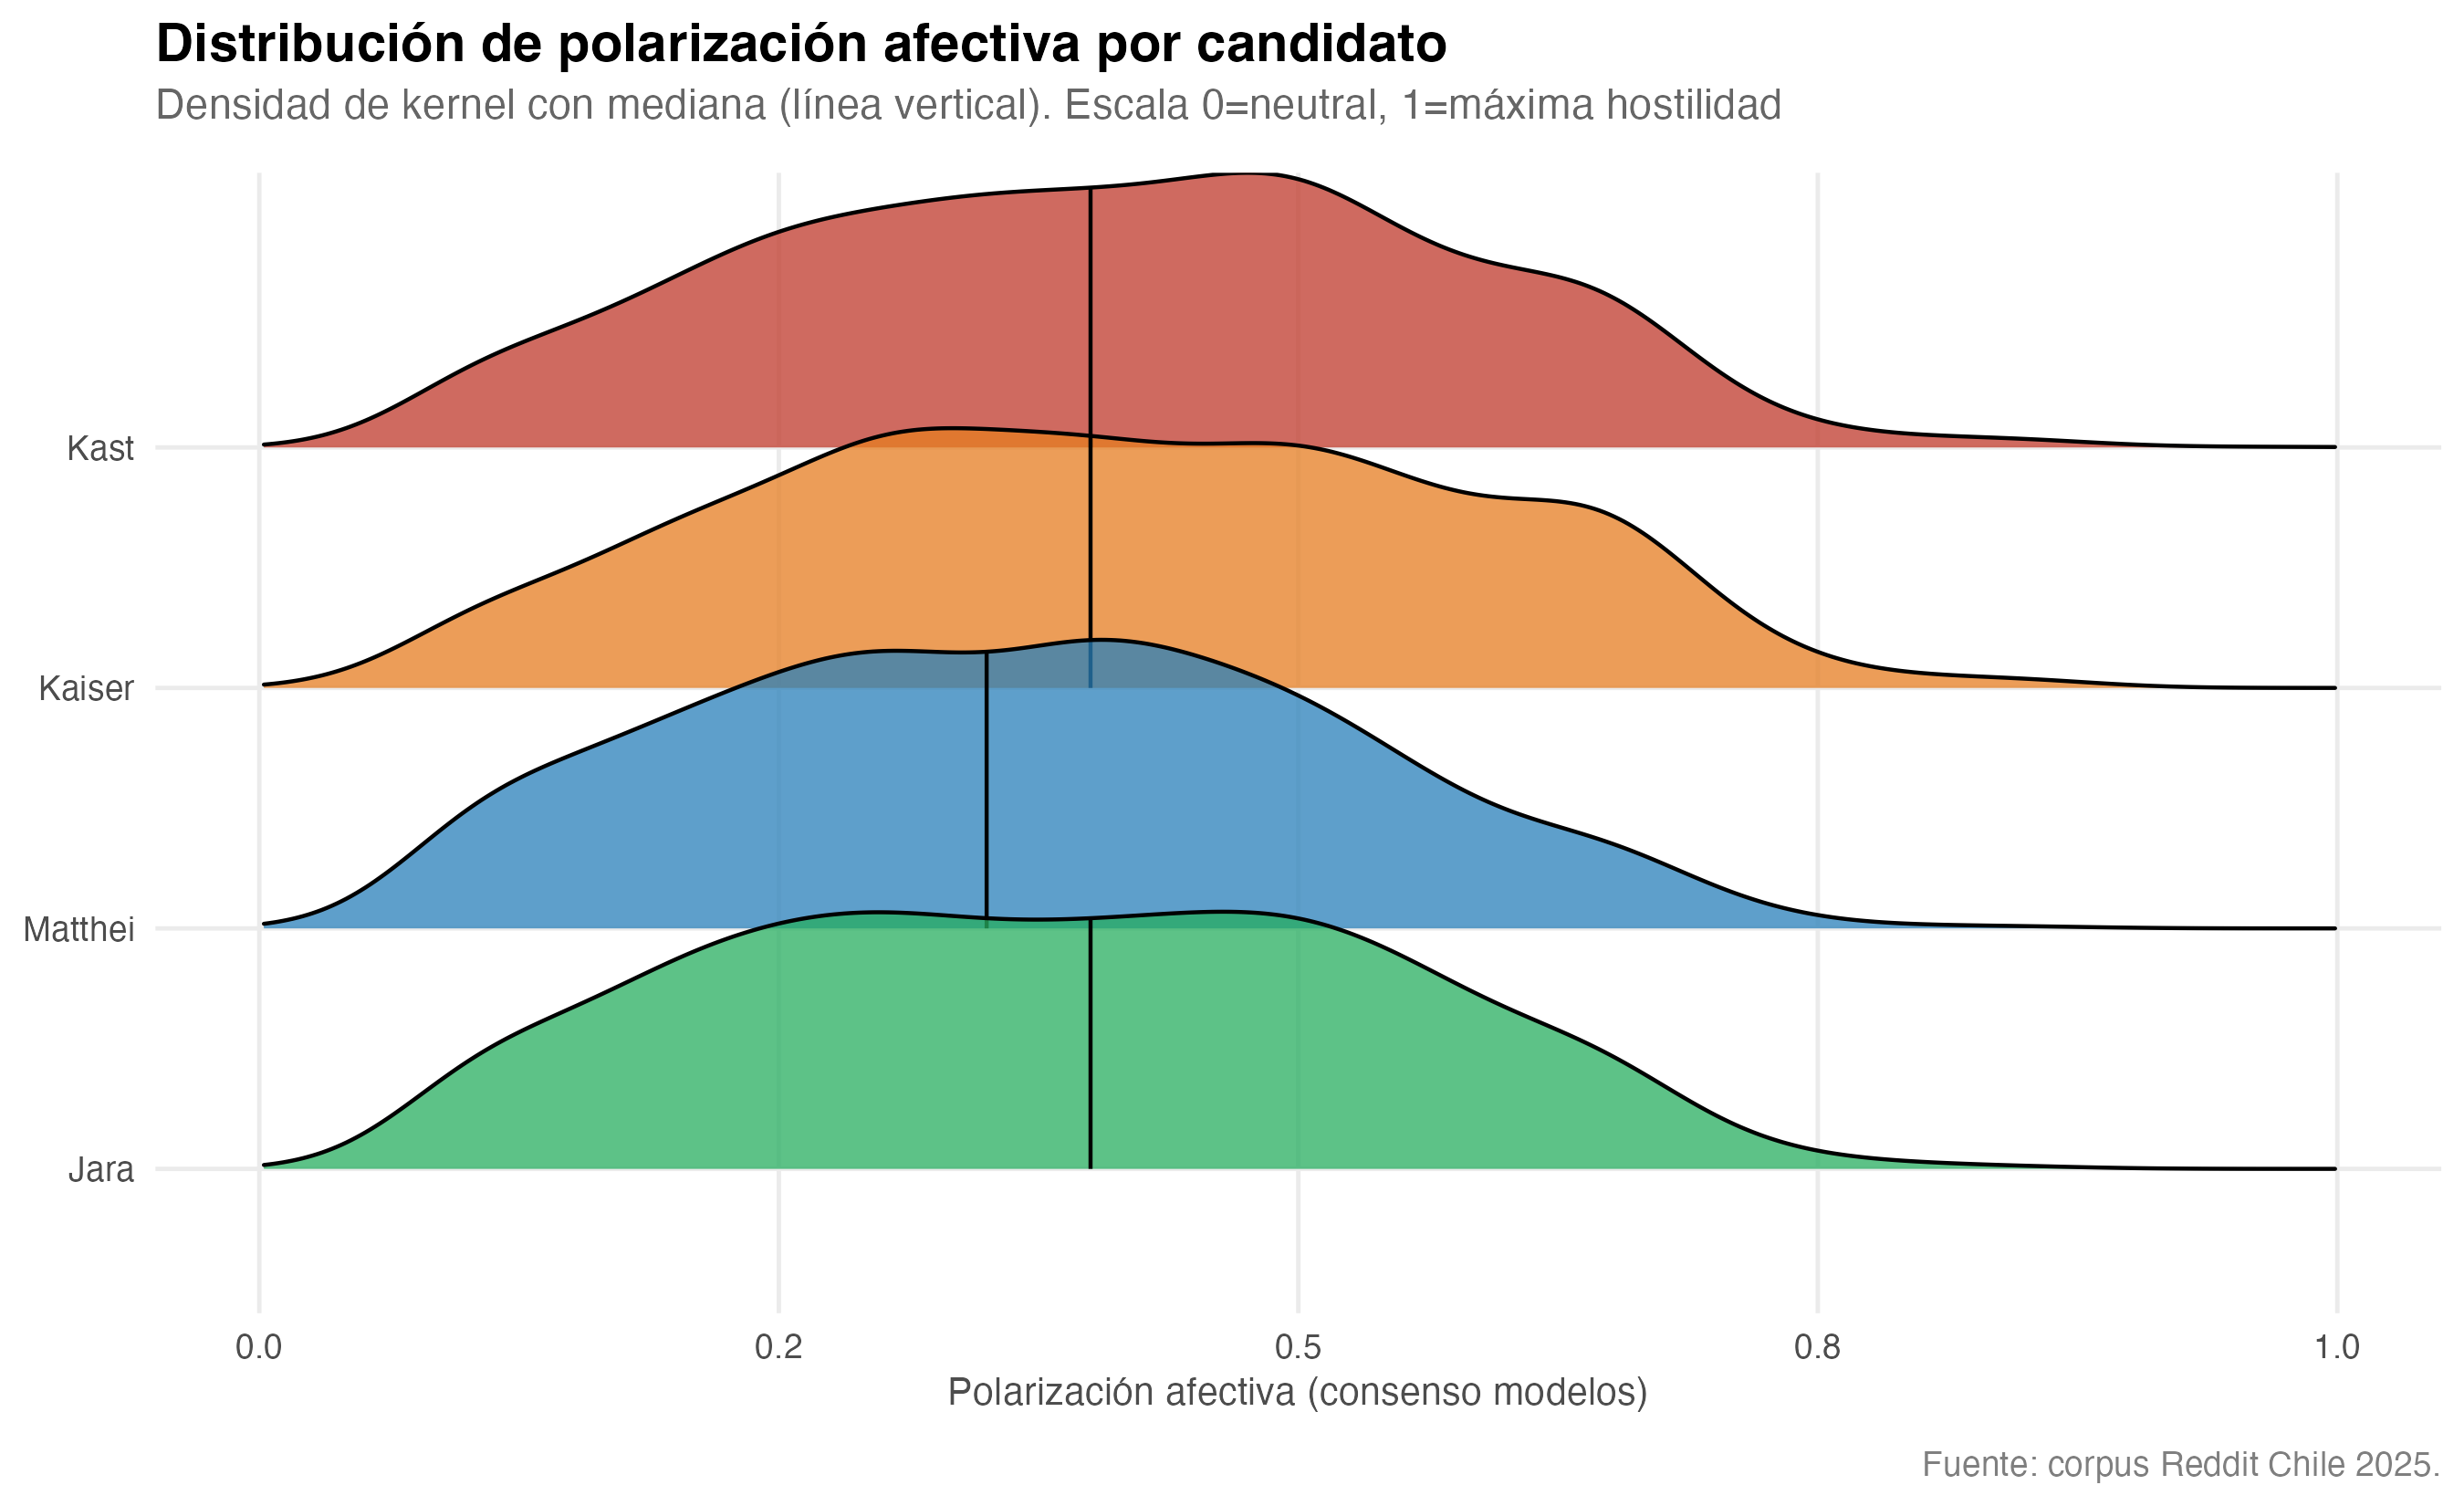
\includegraphics[width=0.92\textwidth,height=\textheight]{fig_thesis/fig7_densidad_polarizacion.png}

}

\caption{\label{fig-explor-densidad-pol}Densidad de polarización por
candidato.}

\end{figure}%

La Figure~\ref{fig-explor-densidad-pol} presenta la distribución de
polarización condicionada al candidato comentado. Los cuatro candidatos
muestran distribuciones unimodales con medianas entre 0.3 y 0.5, pero
con diferencias en dispersión y cola derecha. Kast y Jara exhiben
distribuciones más anchas y con mayor densidad en valores altos de
polarización, mientras que Kaiser y Matthei se concentran en rangos
moderados. Esto es consistente con la mayor visibilidad y carga
adversarial de los dos candidatos que disputaron la segunda vuelta. Que
ningún candidato presente una distribución bimodal sugiere que la
polarización opera como un gradiente continuo, no como una dicotomía
entre comentarios hostiles y no hostiles.

\section{Emociones en el tiempo (facetas por
candidato)}\label{emociones-en-el-tiempo-facetas-por-candidato}

\begin{figure}[H]

\centering{

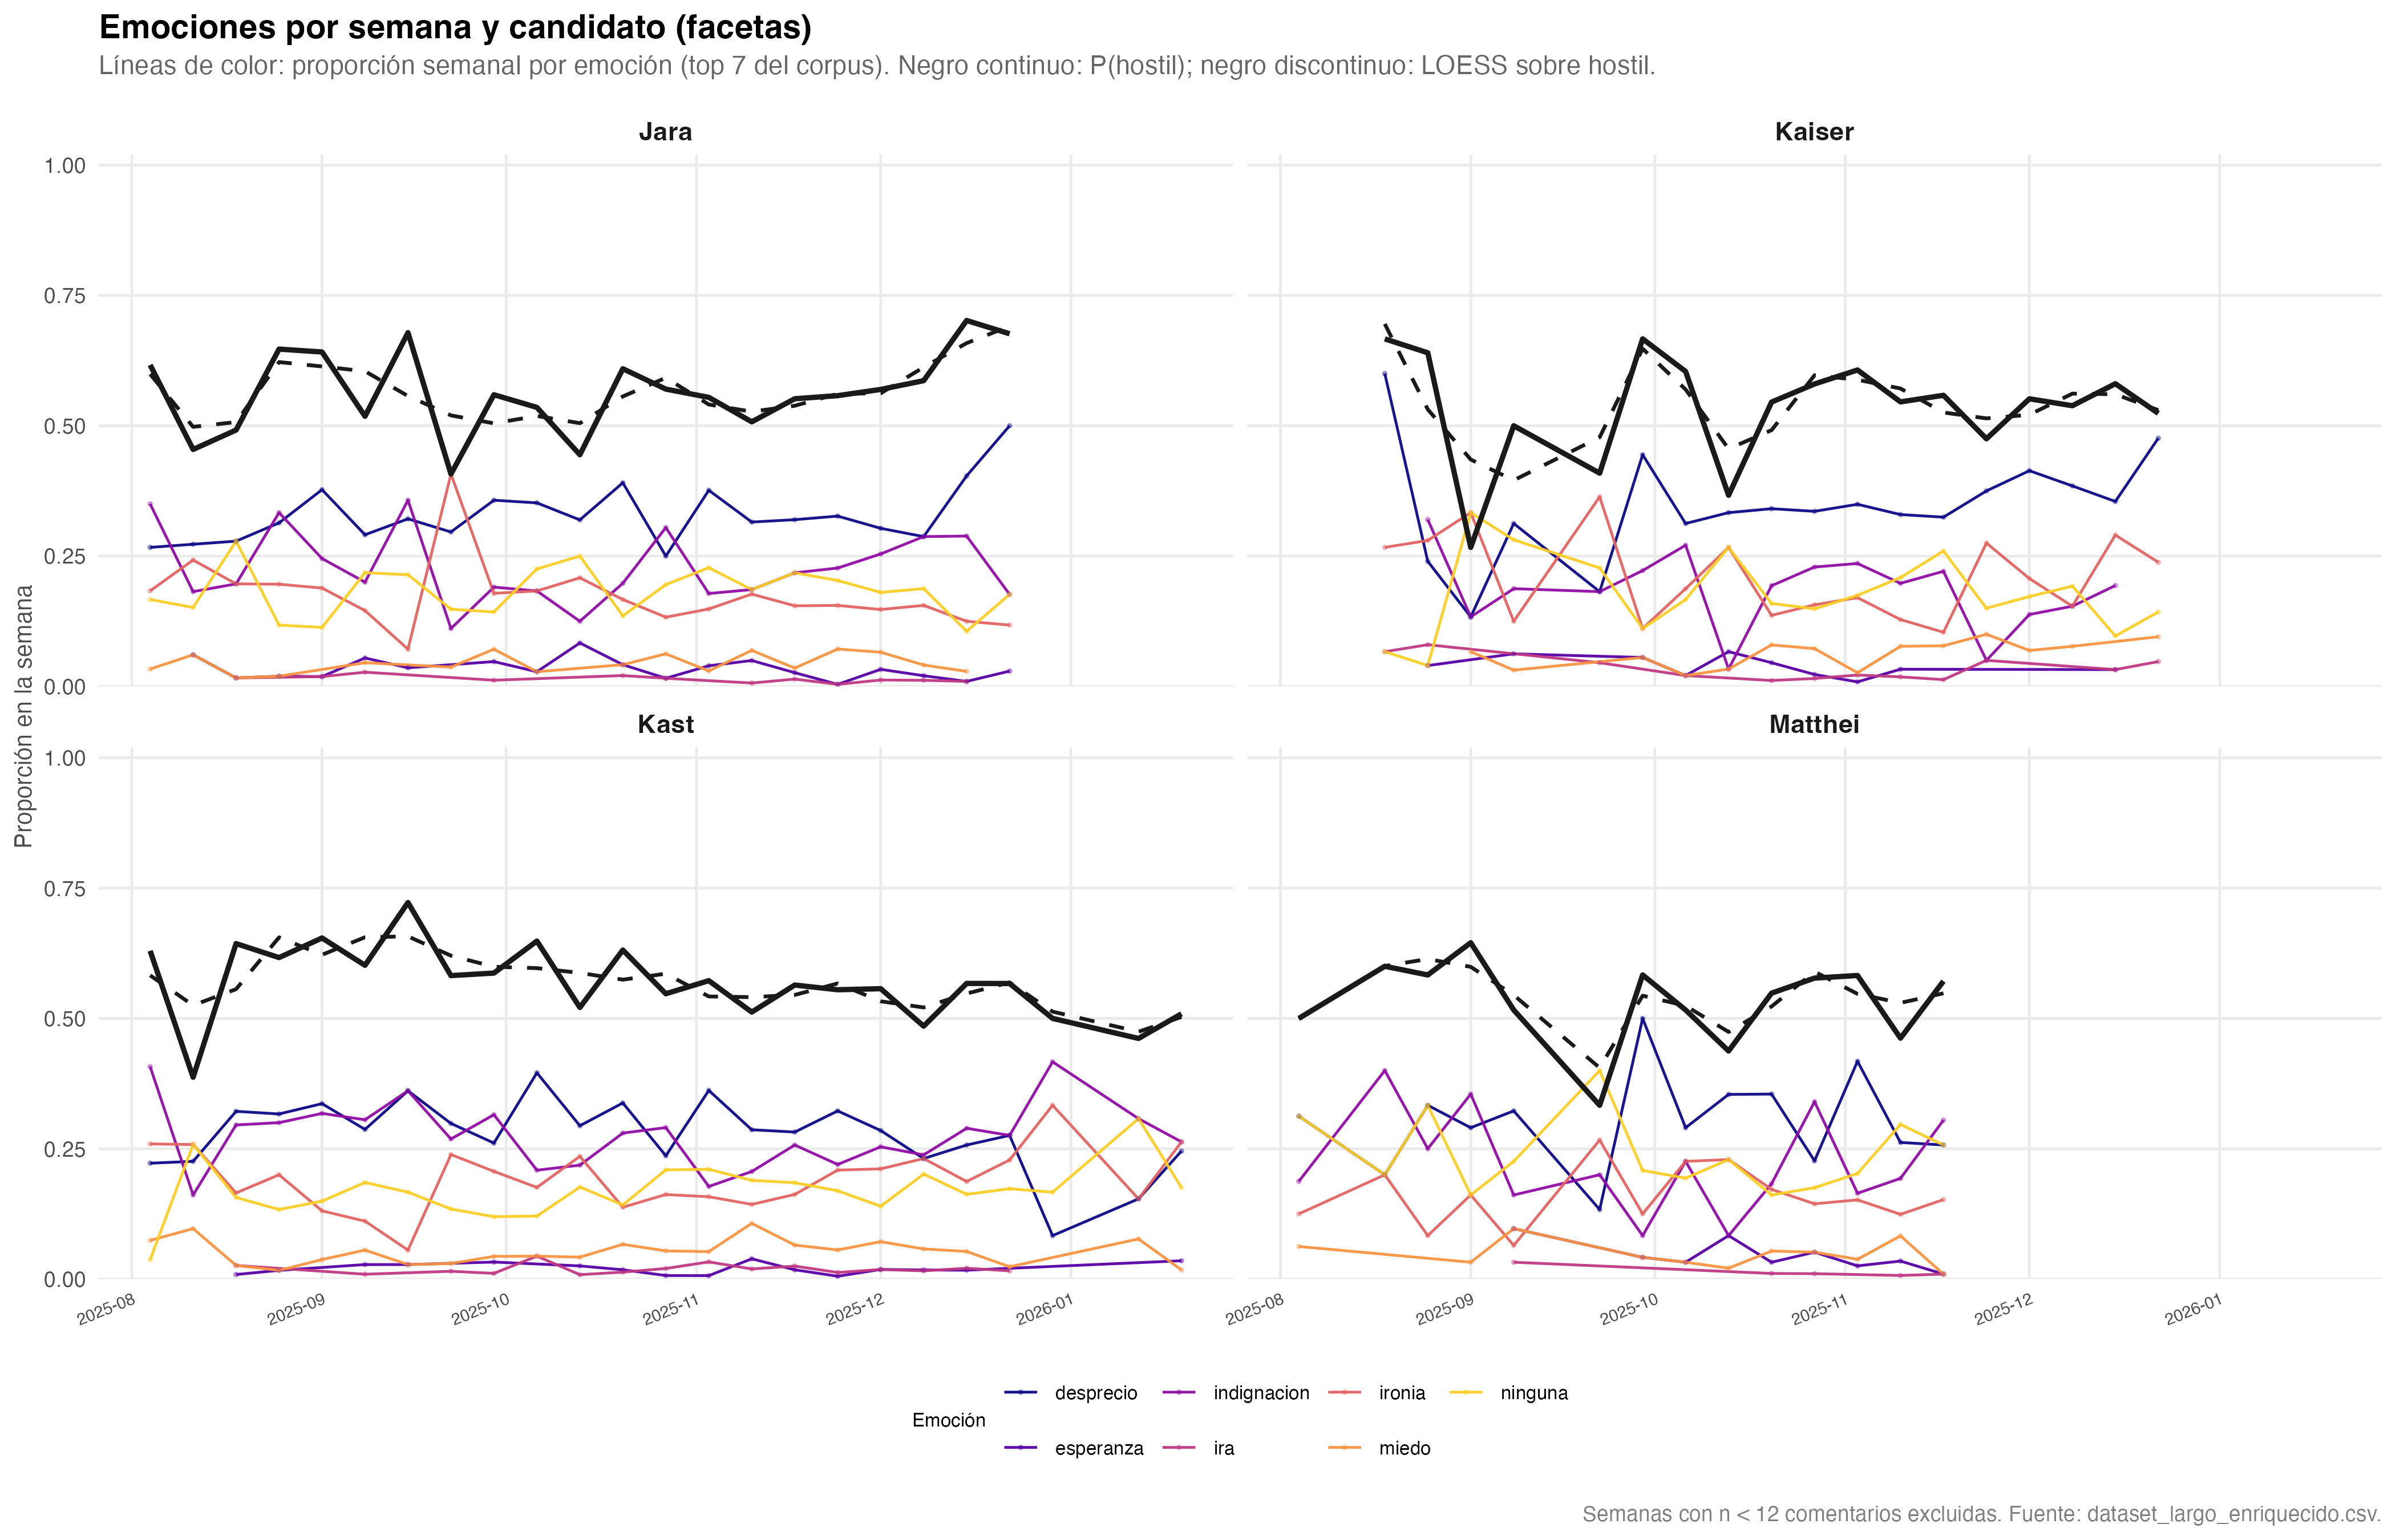
\includegraphics[width=1\textwidth,height=\textheight]{images/emociones_candidato_semanal_facet_tendencia.png}

}

\caption{\label{fig-emociones-candidato-tendencia}Emociones semanales
por candidato (facetas 2×2).}

\end{figure}%

La Figure~\ref{fig-emociones-candidato-tendencia} muestra, para cada
candidato, la proporción semanal de las emociones más frecuentes en el
corpus. La línea negra continua representa la fracción de emociones
hostiles (ira, desprecio, indignación); el trazo discontinuo es un
suavizado LOESS sobre esa fracción. Dos patrones merecen atención.
Primero, la proporción de hostilidad se mantiene relativamente estable a
lo largo del ciclo para los cuatro candidatos --- no hay un escalamiento
progresivo hacia la elección, sino una hostilidad de base que fluctúa en
torno a un nivel constante. Segundo, Kast presenta los picos de
hostilidad más pronunciados, coincidentes con semanas de alta actividad
mediática, mientras que Matthei muestra la fracción hostil más baja y
menos volátil. El desprecio y la indignación alternan como emociones
dominantes según el candidato, lo que anticipa el hallazgo del capítulo
8 sobre la relevancia de las \emph{configuraciones discursivas}
(combinaciones marco × emoción) por sobre las emociones aisladas.

\section{Polarización en el tiempo}\label{polarizaciuxf3n-en-el-tiempo}

\begin{figure}[H]

\centering{


\includegraphics[width=1\textwidth,height=\textheight]{images/serie_polarizacion_candidatos.png}

}

\caption{\label{fig-explor-pol-serie}Polarización media cada dos días
por candidato.}

\end{figure}%

La Figure~\ref{fig-explor-pol-serie} reproduce la serie bisegmentada
(cada dos días) de polarización media por candidato, con bandas de IC
95\%. Las cuatro series oscilan entre 0.3 y 0.5, sin una tendencia
ascendente clara hacia la elección. Kast y Jara mantienen los niveles
más altos durante la mayor parte del período, con una convergencia
notable a partir de noviembre cuando la competencia se reduce a estos
dos candidatos. Kaiser y Matthei desaparecen de la serie tras la primera
vuelta. Las bandas de confianza se estrechan en las semanas de mayor
volumen y se ensanchan en períodos de baja actividad, lo que refleja la
variabilidad muestral más que cambios reales en la hostilidad. En
conjunto, la serie temporal sugiere estabilidad estructural de la
polarización --- un hallazgo que el capítulo 7 formaliza mediante
validación cruzada y el capítulo 8 interpreta como cristalización
actitudinal.

\bookmarksetup{startatroot}

\chapter{Modelado de Datos}\label{modelado-de-datos}

Se aplicó\ldots{}

\section{Consistencia de medición}\label{consistencia-de-mediciuxf3n}

\subsection{Acuerdo entre anotadores
automáticos}\label{acuerdo-entre-anotadores-automuxe1ticos}

Antes de utilizar las variables discursivas como predictores, es
necesario establecer en qué medida los dos sistemas de clasificación
automática ---OpenAI (OA) y DeepSeek (DS)--- producen resultados
convergentes. Si el acuerdo entre ambos fuera sistemáticamente bajo, las
variables resultantes podrían reflejar idiosincrasias del modelo más que
propiedades del texto. La siguiente tabla resume el acuerdo por
dimensión.

La polarización alcanza r = 0.665, lo que indica una convergencia
moderada-alta entre ambos sistemas en la dimensión continua. Si bien
esta correlación no es directamente comparable con estudios de acuerdo
inter-anotador humano ---que operan bajo condiciones de instrucción y
contexto distintas---, el nivel de convergencia sugiere que ambos
modelos capturan una señal compartida en la evaluación de hostilidad
discursiva.

Para las dimensiones categóricas el panorama es más heterogéneo.
Estrategia presenta la coincidencia bruta más alta (61.2\%) pero un
kappa bajo (κ = 0.126), lo cual refleja una distribución desbalanceada
donde la categoría mayoritaria infla la coincidencia sin elevar el
acuerdo ajustado por azar. Frontera muestra un kappa negativo (κ =
−0.146), un resultado que puede parecer paradójico pero que se explica
por la estructura del desacuerdo: ambos sistemas tienden a identificar
los mismos comentarios como fronterizos, pero discrepan de manera
sistemática sobre la dirección de esa frontera (inter-bloque
vs.~intra-bloque), lo que genera un patrón de desacuerdo no aleatorio
que el estadístico kappa penaliza con valores negativos. Marco y emoción
registran los acuerdos más bajos (κ = 0.136 y κ = 0.076,
respectivamente), consistente con la mayor ambigüedad inherente a estas
categorías: un mismo comentario admite lecturas legítimas en más de una
categoría ---por ejemplo, como indignación o desprecio, o encuadrado en
un marco de conflicto o diagnóstico---, sin que ninguna de las dos
lecturas sea incorrecta.

Estos valores de kappa no invalidan el sistema de medición, pero sí
delimitan su alcance interpretativo. La estrategia adoptada en esta
tesis es el desempate por consenso (v5.1), donde la etiqueta final se
asigna por acuerdo entre modelos y, en caso de discrepancia, se prioriza
la clasificación del modelo con mayor karma acumulado en la dimensión
correspondiente. Las dimensiones con bajo acuerdo inter-modelo no se
descartan, sino que se incorporan con la cautela analítica que su nivel
de estabilidad exige.

\subsection{Modelo de desacuerdo}\label{modelo-de-desacuerdo}

Para caracterizar las condiciones bajo las cuales ambos sistemas
discrepan, se entrenó un clasificador binario (acuerdo vs.~desacuerdo)
usando rasgos del comentario como predictores. Los resultados (Anexo A,
Table~\ref{tbl-anexo-desacuerdo}) muestran que el desacuerdo es
parcialmente predecible: RandomForest alcanza un accuracy de 0.680, lo
que sugiere que ciertas propiedades del texto ---como la brevedad, la
ambigüedad tonal o la baja densidad de marcadores explícitos--- aumentan
sistemáticamente la probabilidad de discrepancia entre los anotadores
automáticos.

\subsection{Valor añadido de las variables
discursivas}\label{valor-auxf1adido-de-las-variables-discursivas}

La tabla comparativa de configuraciones (solo TF-IDF, solo variables
LLM, combinado) figura en el Anexo A
(Table~\ref{tbl-anexo-config-features}). La
Figure~\ref{fig-r2-configuraciones} sintetiza el resultado principal.

\begin{figure}[H]

\centering{

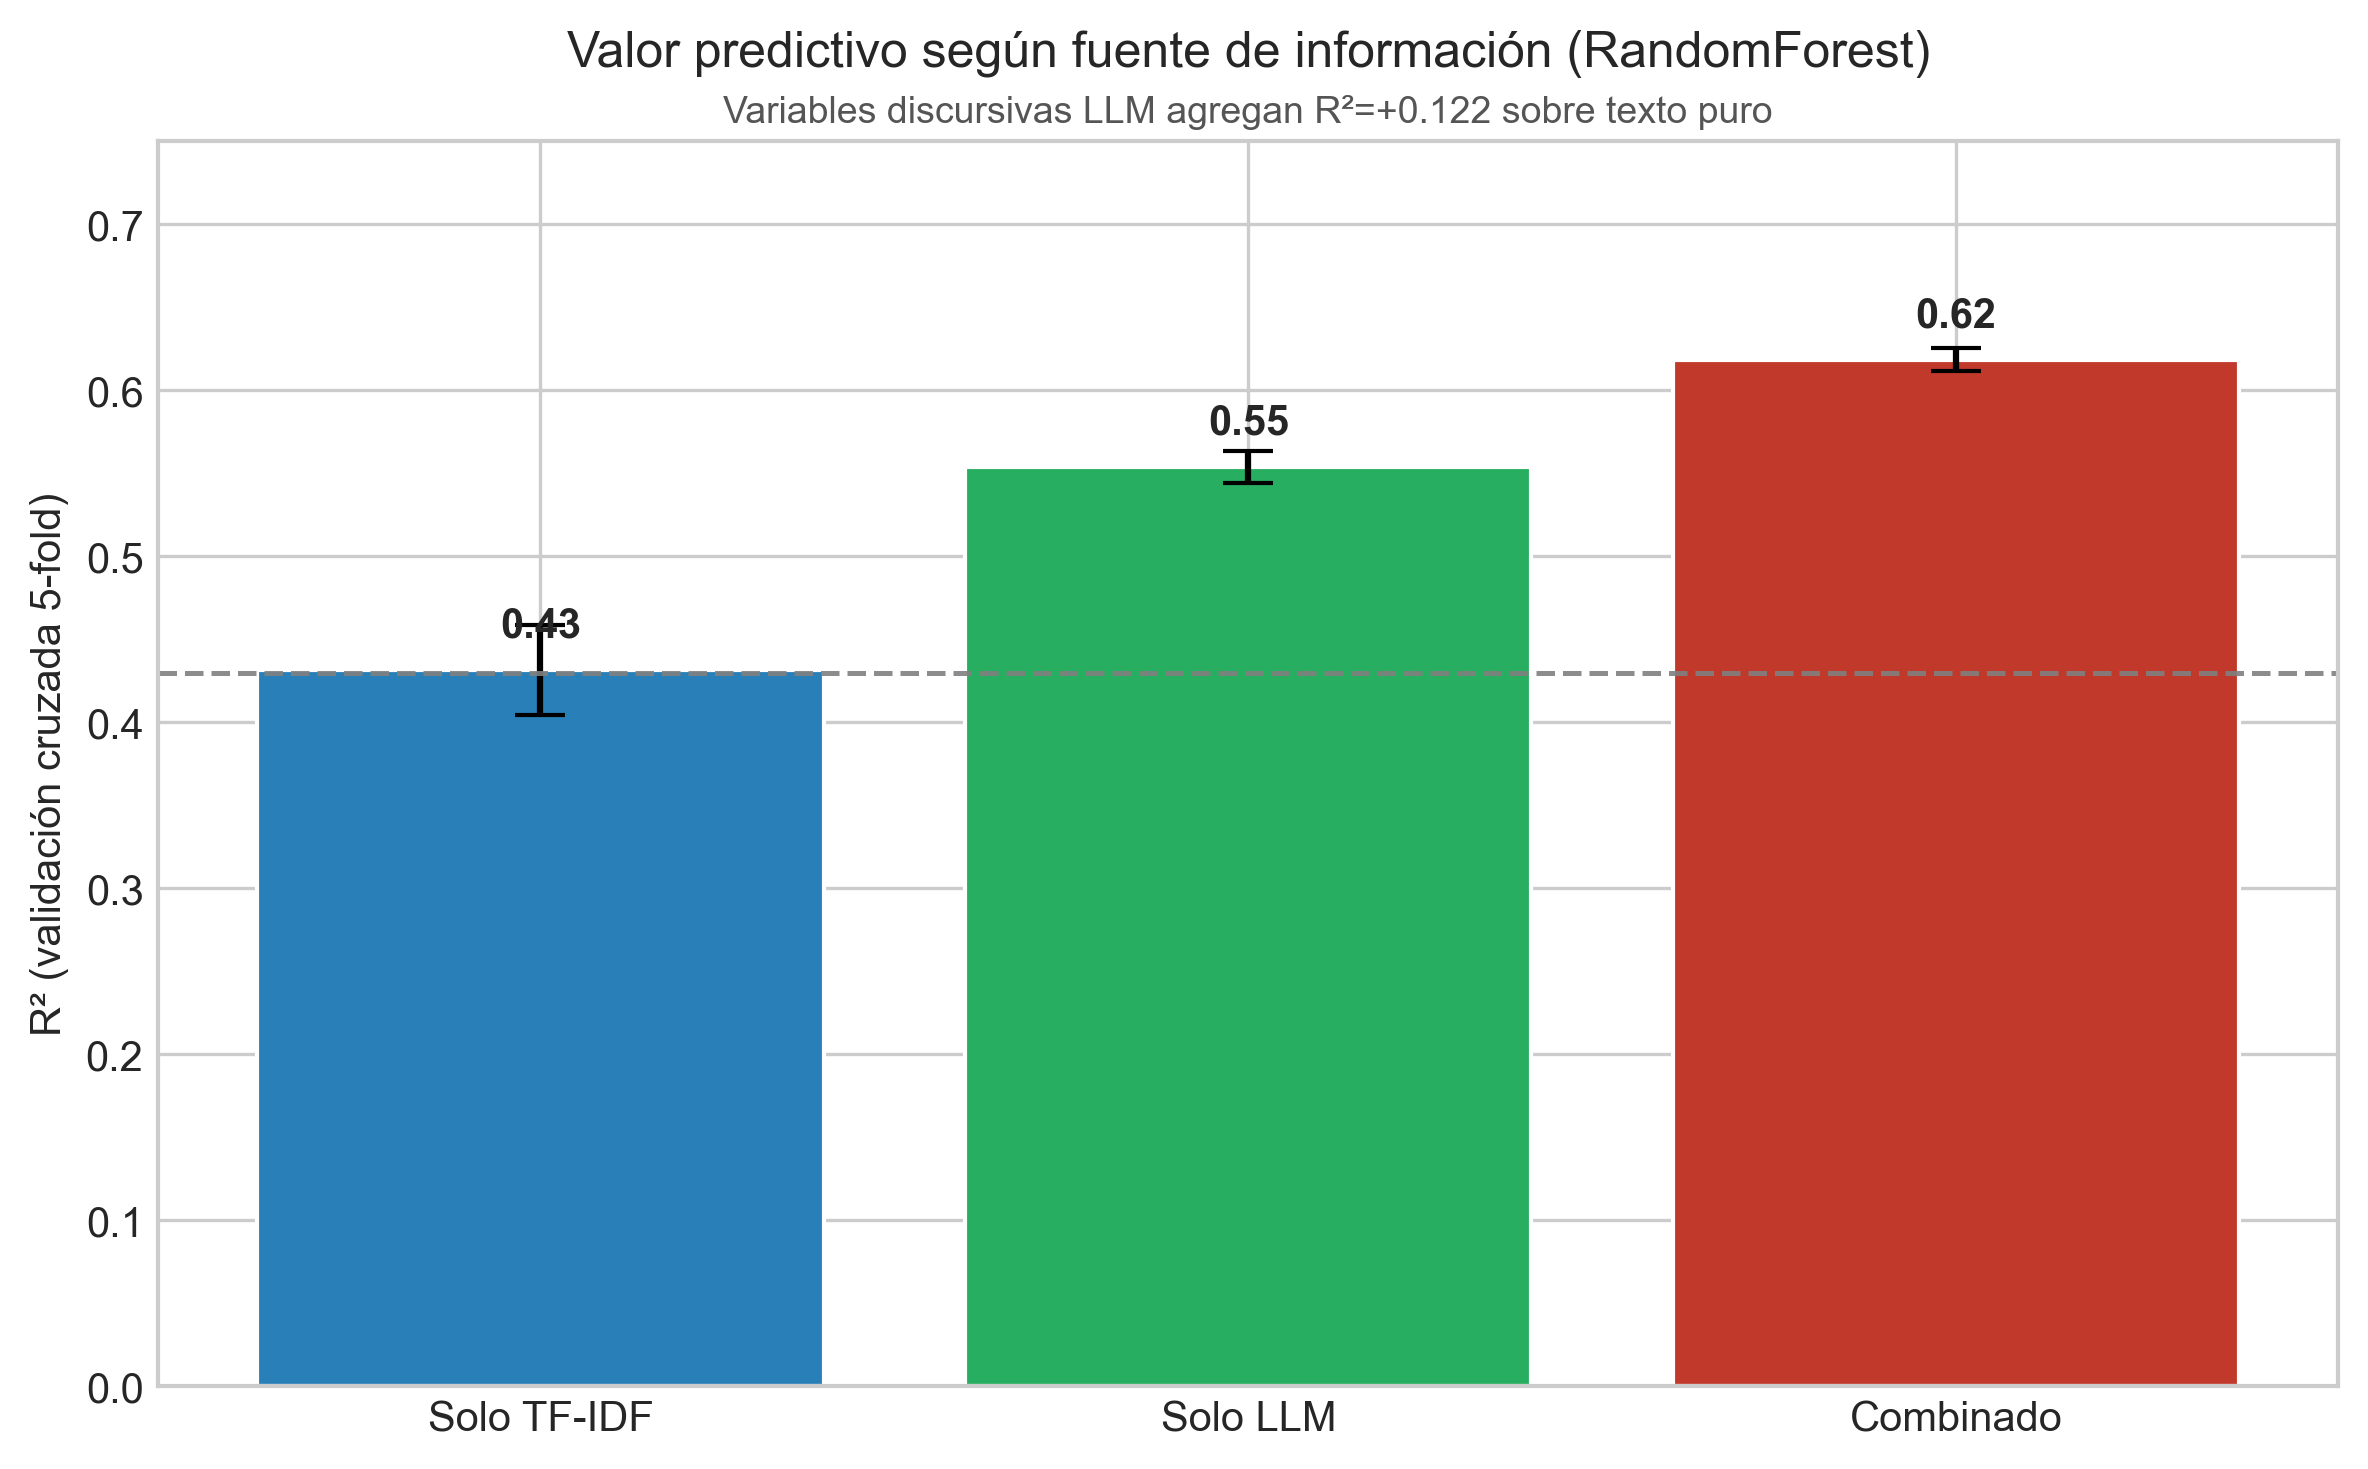
\includegraphics[width=0.85\textwidth,height=\textheight]{fig_thesis/figura_r2_configuraciones.png}

}

\caption{\label{fig-r2-configuraciones}Comparación de R² por
configuración de variables.}

\end{figure}%

Este resultado constituye el argumento técnico central del capítulo. Si
las variables LLM fueran redundantes respecto del texto crudo, el bloque
discursivo no debería superar al TF-IDF. Sin embargo, las variables LLM
por sí solas alcanzan un R² superior (0.554 vs.~0.432), y en combinación
con TF-IDF el rendimiento sube a R² = 0.618 --- un incremento de +0.187
sobre el texto puro. Esto sugiere que el sistema no solo recodifica la
información ya presente en el texto, sino que recupera estructura
discursiva adicional que las representaciones de bolsa de palabras no
capturan.

\subsection{Calibración de
probabilidades}\label{calibraciuxf3n-de-probabilidades}

El diagrama de fiabilidad (Figure~\ref{fig-reliability}) muestra que
tanto RandomForest como GBM se aproximan a la diagonal de calibración
perfecta. RandomForest sin calibrar ya presenta un ajuste razonable,
mientras que GBM mejora marginalmente en el rango medio tras la
corrección isotónica. Esto confirma que el pipeline produce
probabilidades suficientemente confiables sin requerir
post-procesamiento fuerte. Las métricas numéricas (Brier, log-loss) se
detallan en el Anexo A (Table~\ref{tbl-anexo-calibracion}).

\begin{figure}[H]

\centering{

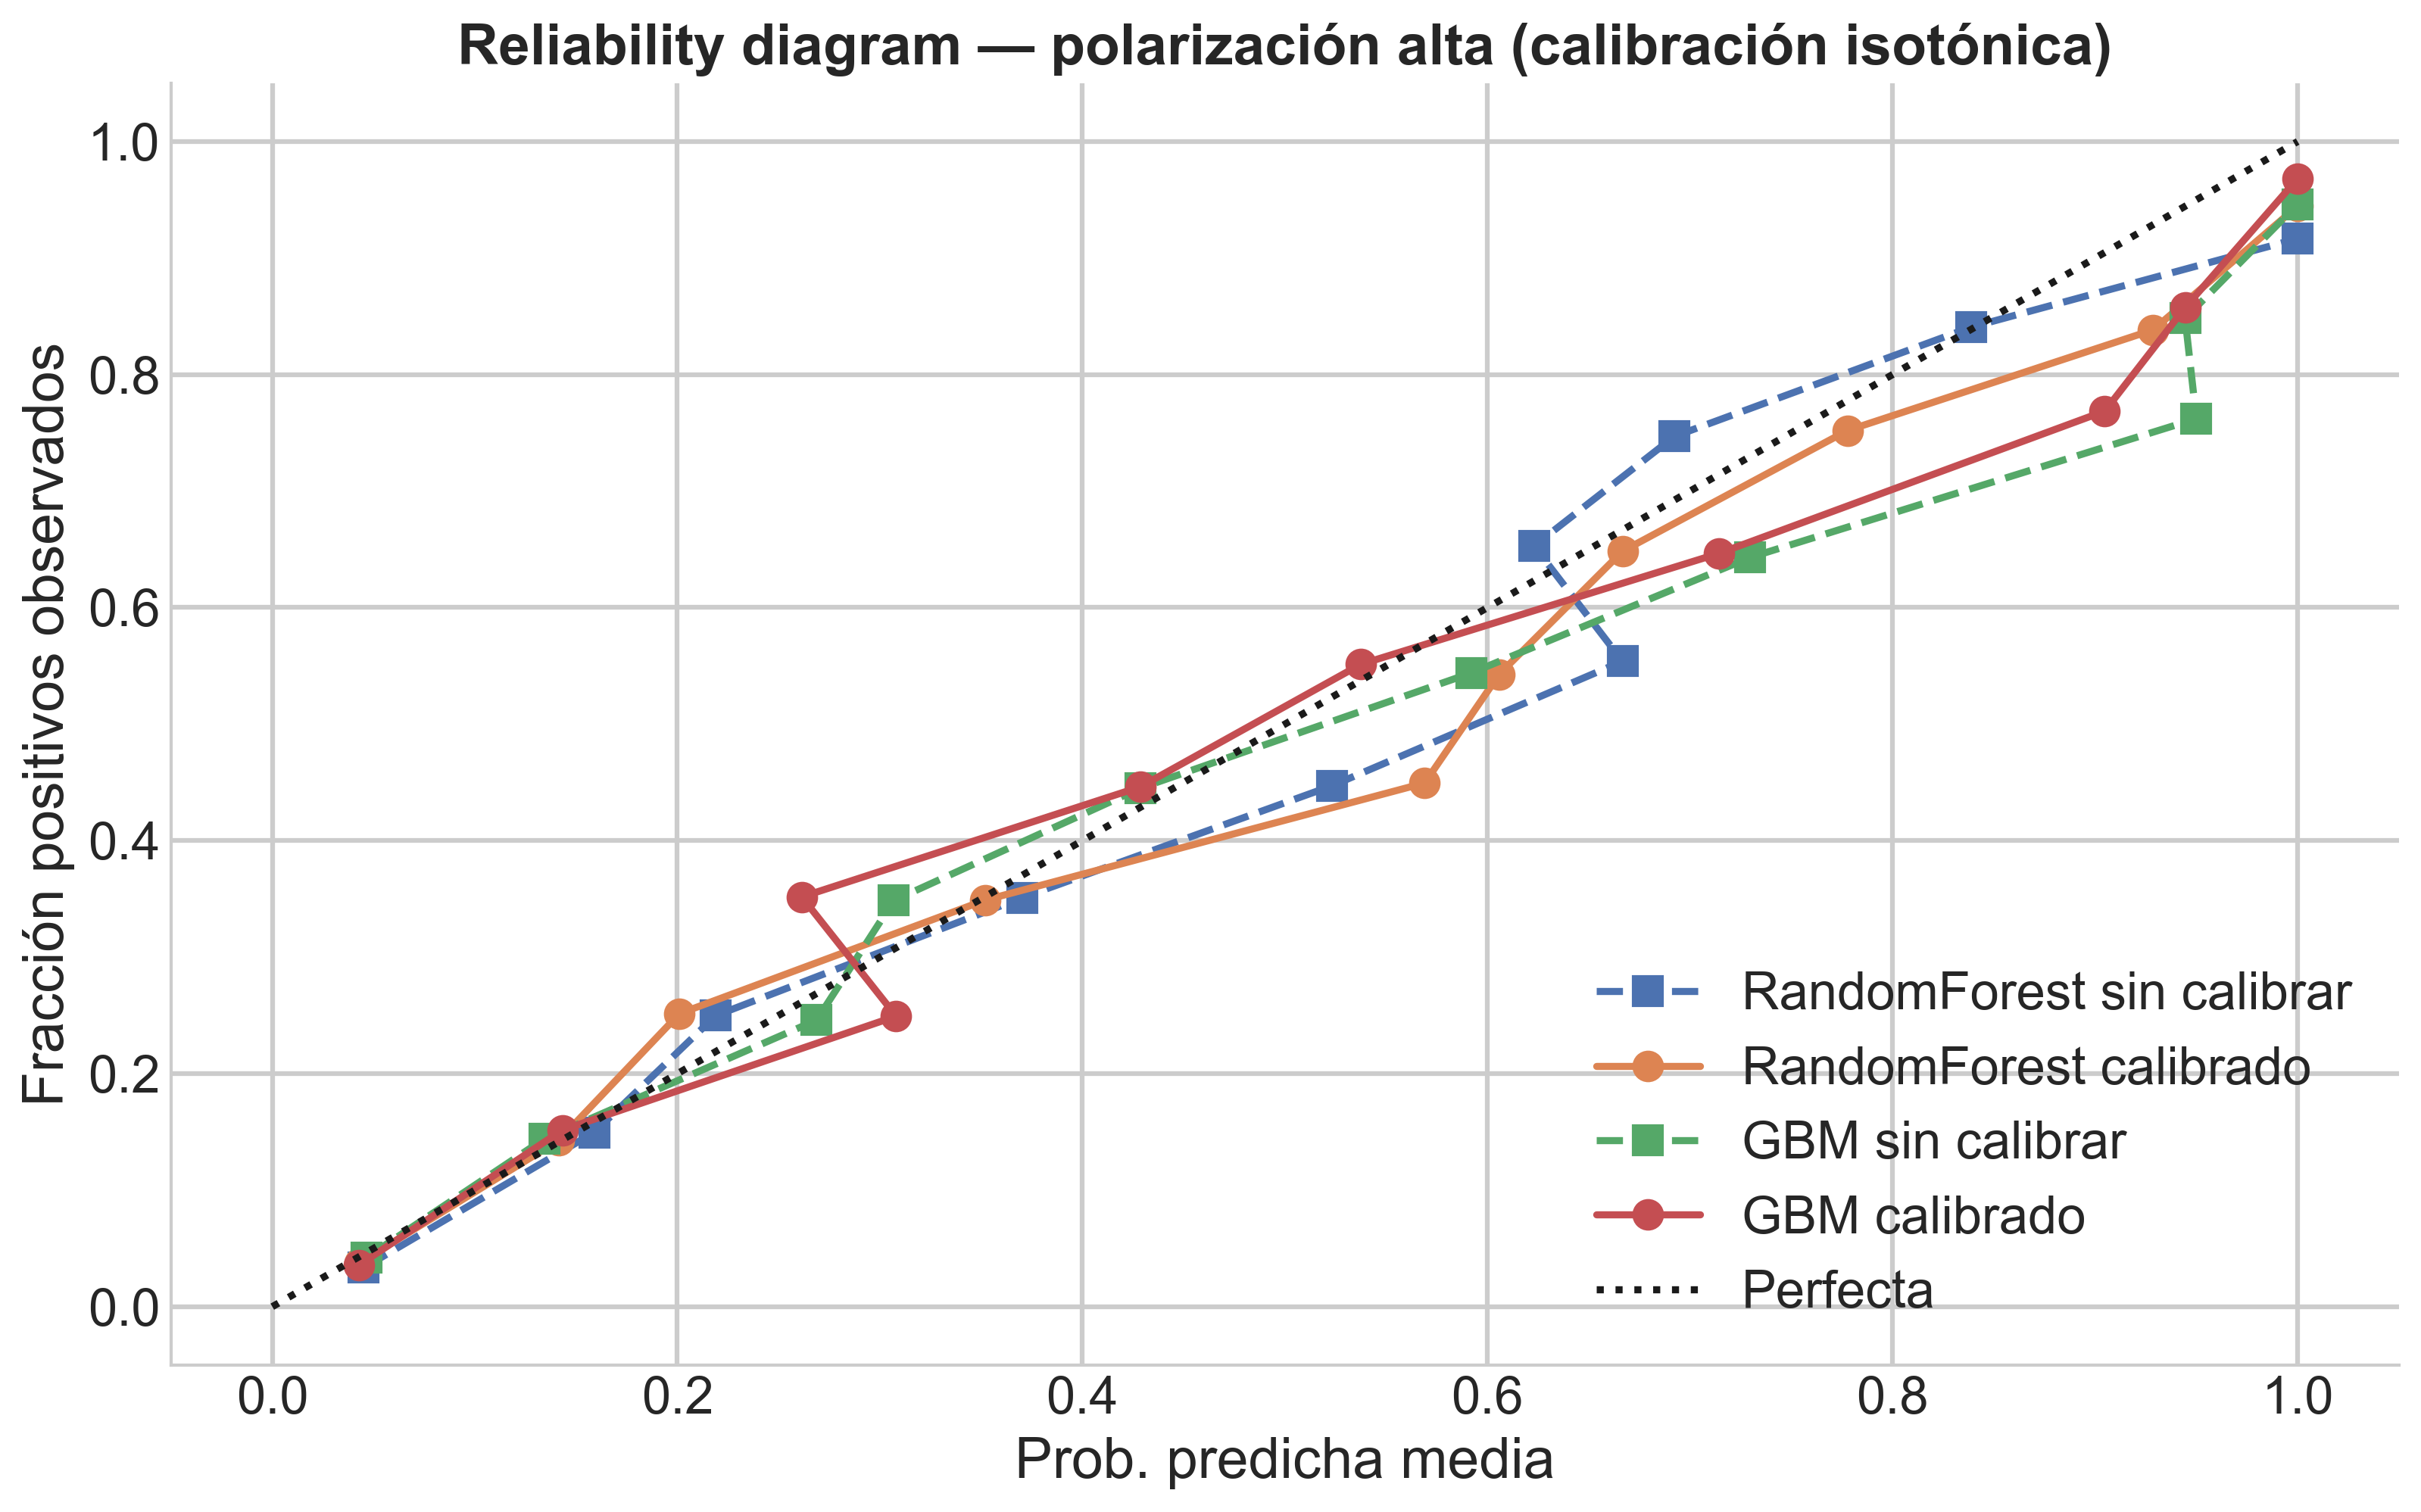
\includegraphics[width=0.82\textwidth,height=\textheight]{fig_thesis/reliability_diagram_calibracion.png}

}

\caption{\label{fig-reliability}Calibración del clasificador de
polarización alta.}

\end{figure}%

Establecida esta base de consistencia y valor añadido, la siguiente
sección examina hasta qué punto estas variables permiten modelar la
polarización de manera robusta fuera de muestra.

\section{Modelado de polarización}\label{modelado-de-polarizaciuxf3n}

\subsection{Evolución temporal (calendario
electoral)}\label{evoluciuxf3n-temporal-calendario-electoral}

El núcleo interpretativo combina \textbf{dos lecturas complementarias}
sobre el mismo corpus: la trayectoria del \textbf{tono negativo} hacia
los dos candidatos de la segunda vuelta (Jara y Kast) y la trayectoria
de la \textbf{polarización discursiva} (consenso entre anotadores) tanto
en esa comparación diaria como en la serie bisegmentada por candidato.
Las figuras se recortan al calendario de la tesis ---tres bloques de
campaña (posicionamiento, primera vuelta, segunda vuelta)---, incluyen
\textbf{referencias de elección} (primera y segunda vuelta) y
\textbf{cierran el 24 de diciembre}, de modo que el postelectoral
inmediato quede visible sin extender la ventana más allá de ese corte.

\subsection{Comparación de modelos y estabilidad fuera de
muestra}\label{comparaciuxf3n-de-modelos-y-estabilidad-fuera-de-muestra}

La Table~\ref{tbl-cv-regresion} compara cuatro estrategias de regresión
evaluadas mediante validación cruzada de cinco pliegues. RandomForest
obtiene el mejor desempeño (R² = 0.619, MAE = 0.084) con la menor
variabilidad entre folds, lo que indica que la señal capturada es
estable y no artefacto de una partición particular. Ridge ofrece un
ajuste competitivo pero inferior, mientras que GBM muestra mayor
inestabilidad (sd = 0.011). El ensamble por stacking eleva el techo
predictivo a R² = 0.646; no obstante, se adopta RandomForest como modelo
de referencia para el resto del capítulo por su combinación de
rendimiento, estabilidad e interpretabilidad.

\begin{longtable}[t]{lll}

\caption{\label{tbl-cv-regresion}Modelos de regresión para
polarización.}

\tabularnewline

\\
\toprule
Modelo & MAE (CV) & R² (CV)\\
\midrule
\cellcolor{gray!10}{Ridge} & \cellcolor{gray!10}{0.098 ± 0.001} & \cellcolor{gray!10}{0.553 ± 0.006}\\
RandomForest & 0.084 ± 0.001 & 0.619 ± 0.006\\
\cellcolor{gray!10}{GBM} & \cellcolor{gray!10}{0.108 ± 0.002} & \cellcolor{gray!10}{0.474 ± 0.011}\\
Stacking &  & 0.646\\
\bottomrule

\end{longtable}

\subsection{OLS interpretable}\label{ols-interpretable}

El OLS no compite con RandomForest en capacidad predictiva, pero cumple
una función complementaria de interpretabilidad: permite inspeccionar la
dirección y magnitud de cada efecto. La tabla de los 15 coeficientes
significativos de mayor magnitud y el coefplot figuran en el Anexo A
(Table~\ref{tbl-anexo-ols-polarizacion} y
Figure~\ref{fig-anexo-coefplot-ols}).

El resultado más relevante es la jerarquía de efectos. La ira domina el
modelo (β = 0.369), seguida por las estrategias adversariales
---ridiculización, amenaza, esencialización y deslegitimación---, todas
con coeficientes positivos entre 0.12 y 0.17. El candidato como target,
en cambio, no aparece entre los 15 predictores más fuertes: su efecto es
estadísticamente nulo (β ≈ 0, p = 0.818). Esto sugiere que la hostilidad
se explica por el \emph{cómo} del discurso ---qué emoción lo sostiene,
qué estrategia lo articula, en qué tipo de hilo ocurre--- y no por el
\emph{quién} es atacado. Se trata de un resultado con implicaciones
teóricas directas para la discusión sobre polarización afectiva, que se
desarrolla en el capítulo siguiente.

\subsection{Importancia por permutación y explicación
local}\label{importancia-por-permutaciuxf3n-y-explicaciuxf3n-local}

La Figure~\ref{fig-perm} confirma desde una perspectiva no paramétrica
lo que el OLS sugiere. El tipo de hilo es la variable con mayor
importancia (caída de R² ≈ 0.50 al permutarla), seguida por estrategia,
número de palabras y emoción, todas con caídas superiores a 0.40. El
candidato, en cambio, ocupa el último lugar con una caída marginal (≈
0.04), lo que refuerza la interpretación de que el target del ataque
resulta prácticamente irrelevante para explicar la intensidad de la
polarización. Notablemente, rasgos textuales brutos como el largo del
comentario (n\_words, n\_chars) ocupan posiciones altas, lo que
contribuye a explicar por qué el modelo combinado supera al puramente
discursivo: la extensión del texto captura información que las etiquetas
categóricas no recogen.

\begin{figure}[H]

\centering{

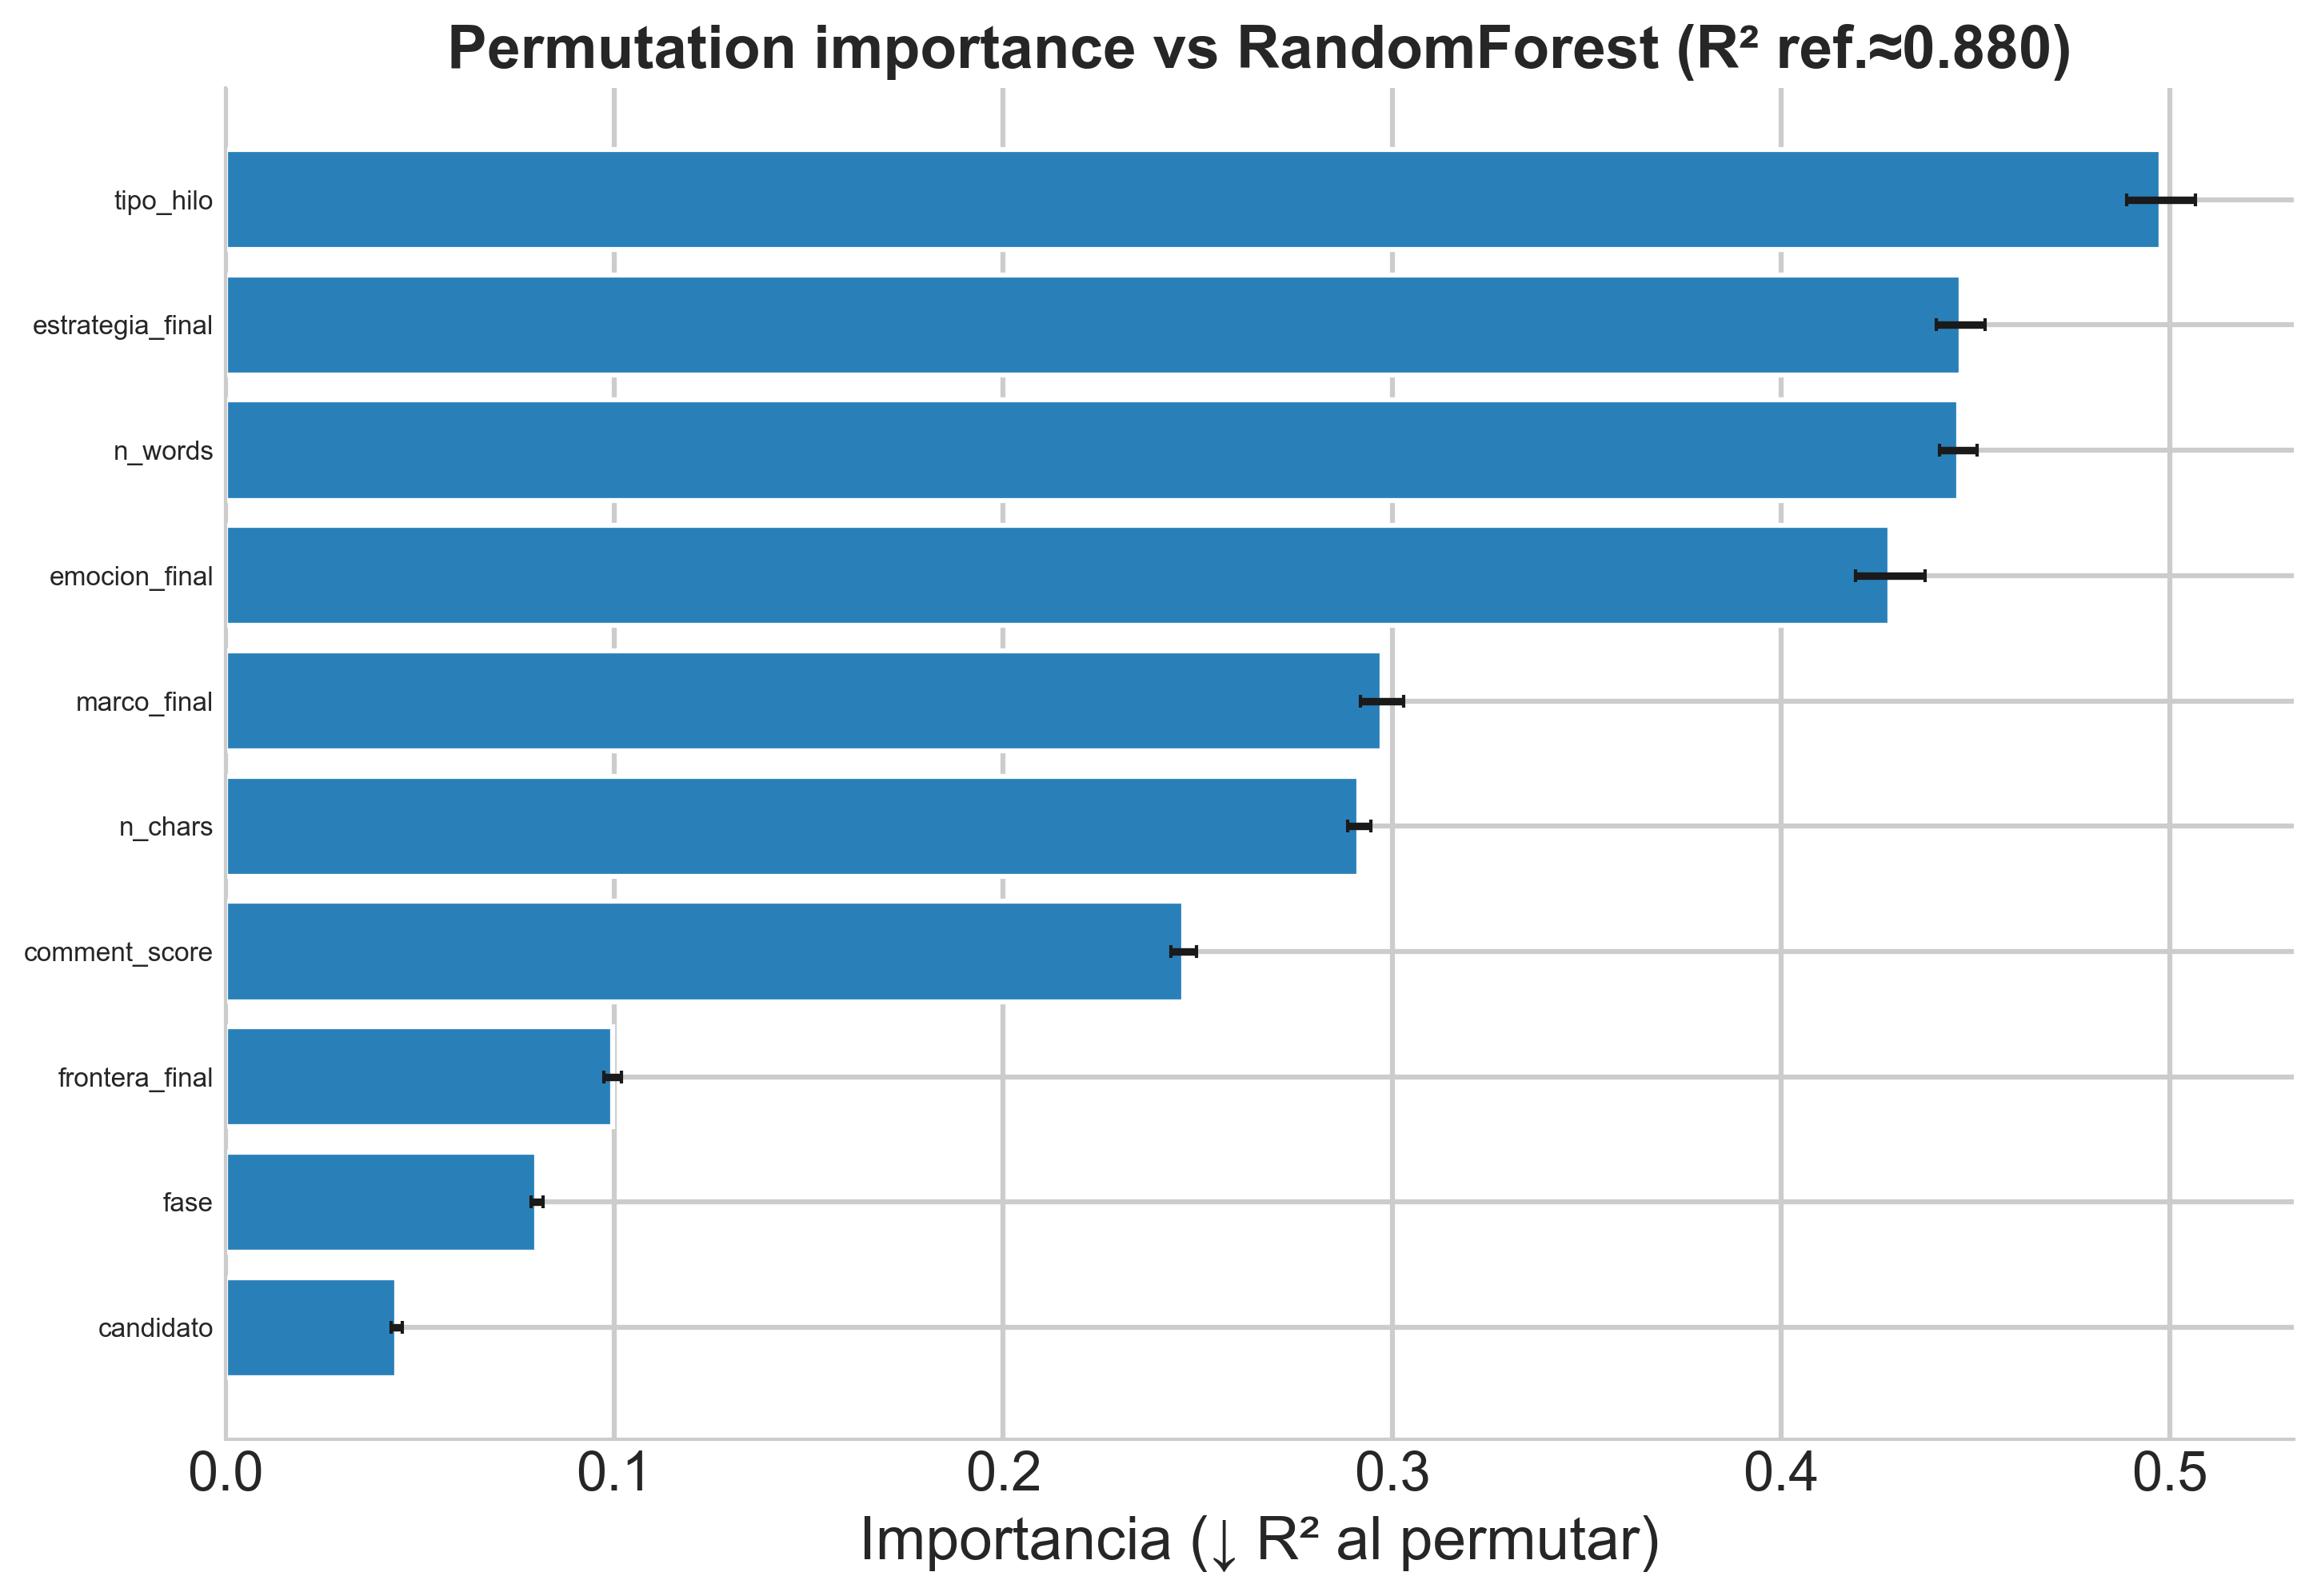
\includegraphics[width=0.82\textwidth,height=\textheight]{fig_thesis/permutation_importance_polarizacion.png}

}

\caption{\label{fig-perm}Importancia por permutación en el modelo de
polarización.}

\end{figure}%

\subsection{Clasificación de polarización
alta}\label{clasificaciuxf3n-de-polarizaciuxf3n-alta}

Para complementar el análisis de regresión, se discretizó la
polarización en un problema binario (umbral ≥ 0.6) y se evaluaron tres
clasificadores. Las curvas ROC (Figure~\ref{fig-roc}) muestran que todos
superan ampliamente la línea aleatoria, con AUCs entre 0.811 (LogReg) y
0.856 (RandomForest). Que un modelo lineal alcance un AUC de 0.81 indica
que buena parte de la señal de hostilidad es linealmente separable: las
emociones y estrategias adversariales, por sí solas, trazan una frontera
razonable entre comentarios de alta y baja polarización. El incremento
adicional de RandomForest (+0.045) sugiere que existen interacciones no
aditivas entre variables discursivas ---por ejemplo, la combinación de
ira con ridiculización en hilos mixtos podría producir niveles de
polarización que no se explican por la suma de sus efectos
individuales---. GBM queda en una posición intermedia (AUC = 0.832),
consistente con su menor estabilidad observada en la regresión. En
conjunto, estos resultados indican que la polarización alta es un
fenómeno clasificable con precisión moderada-alta, pero cuya estructura
heterogénea se beneficia de modelos capaces de capturar no linealidades.
Los valores AUC por modelo se detallan en el Anexo A
(Table~\ref{tbl-anexo-auc}).

\begin{figure}[H]

\centering{

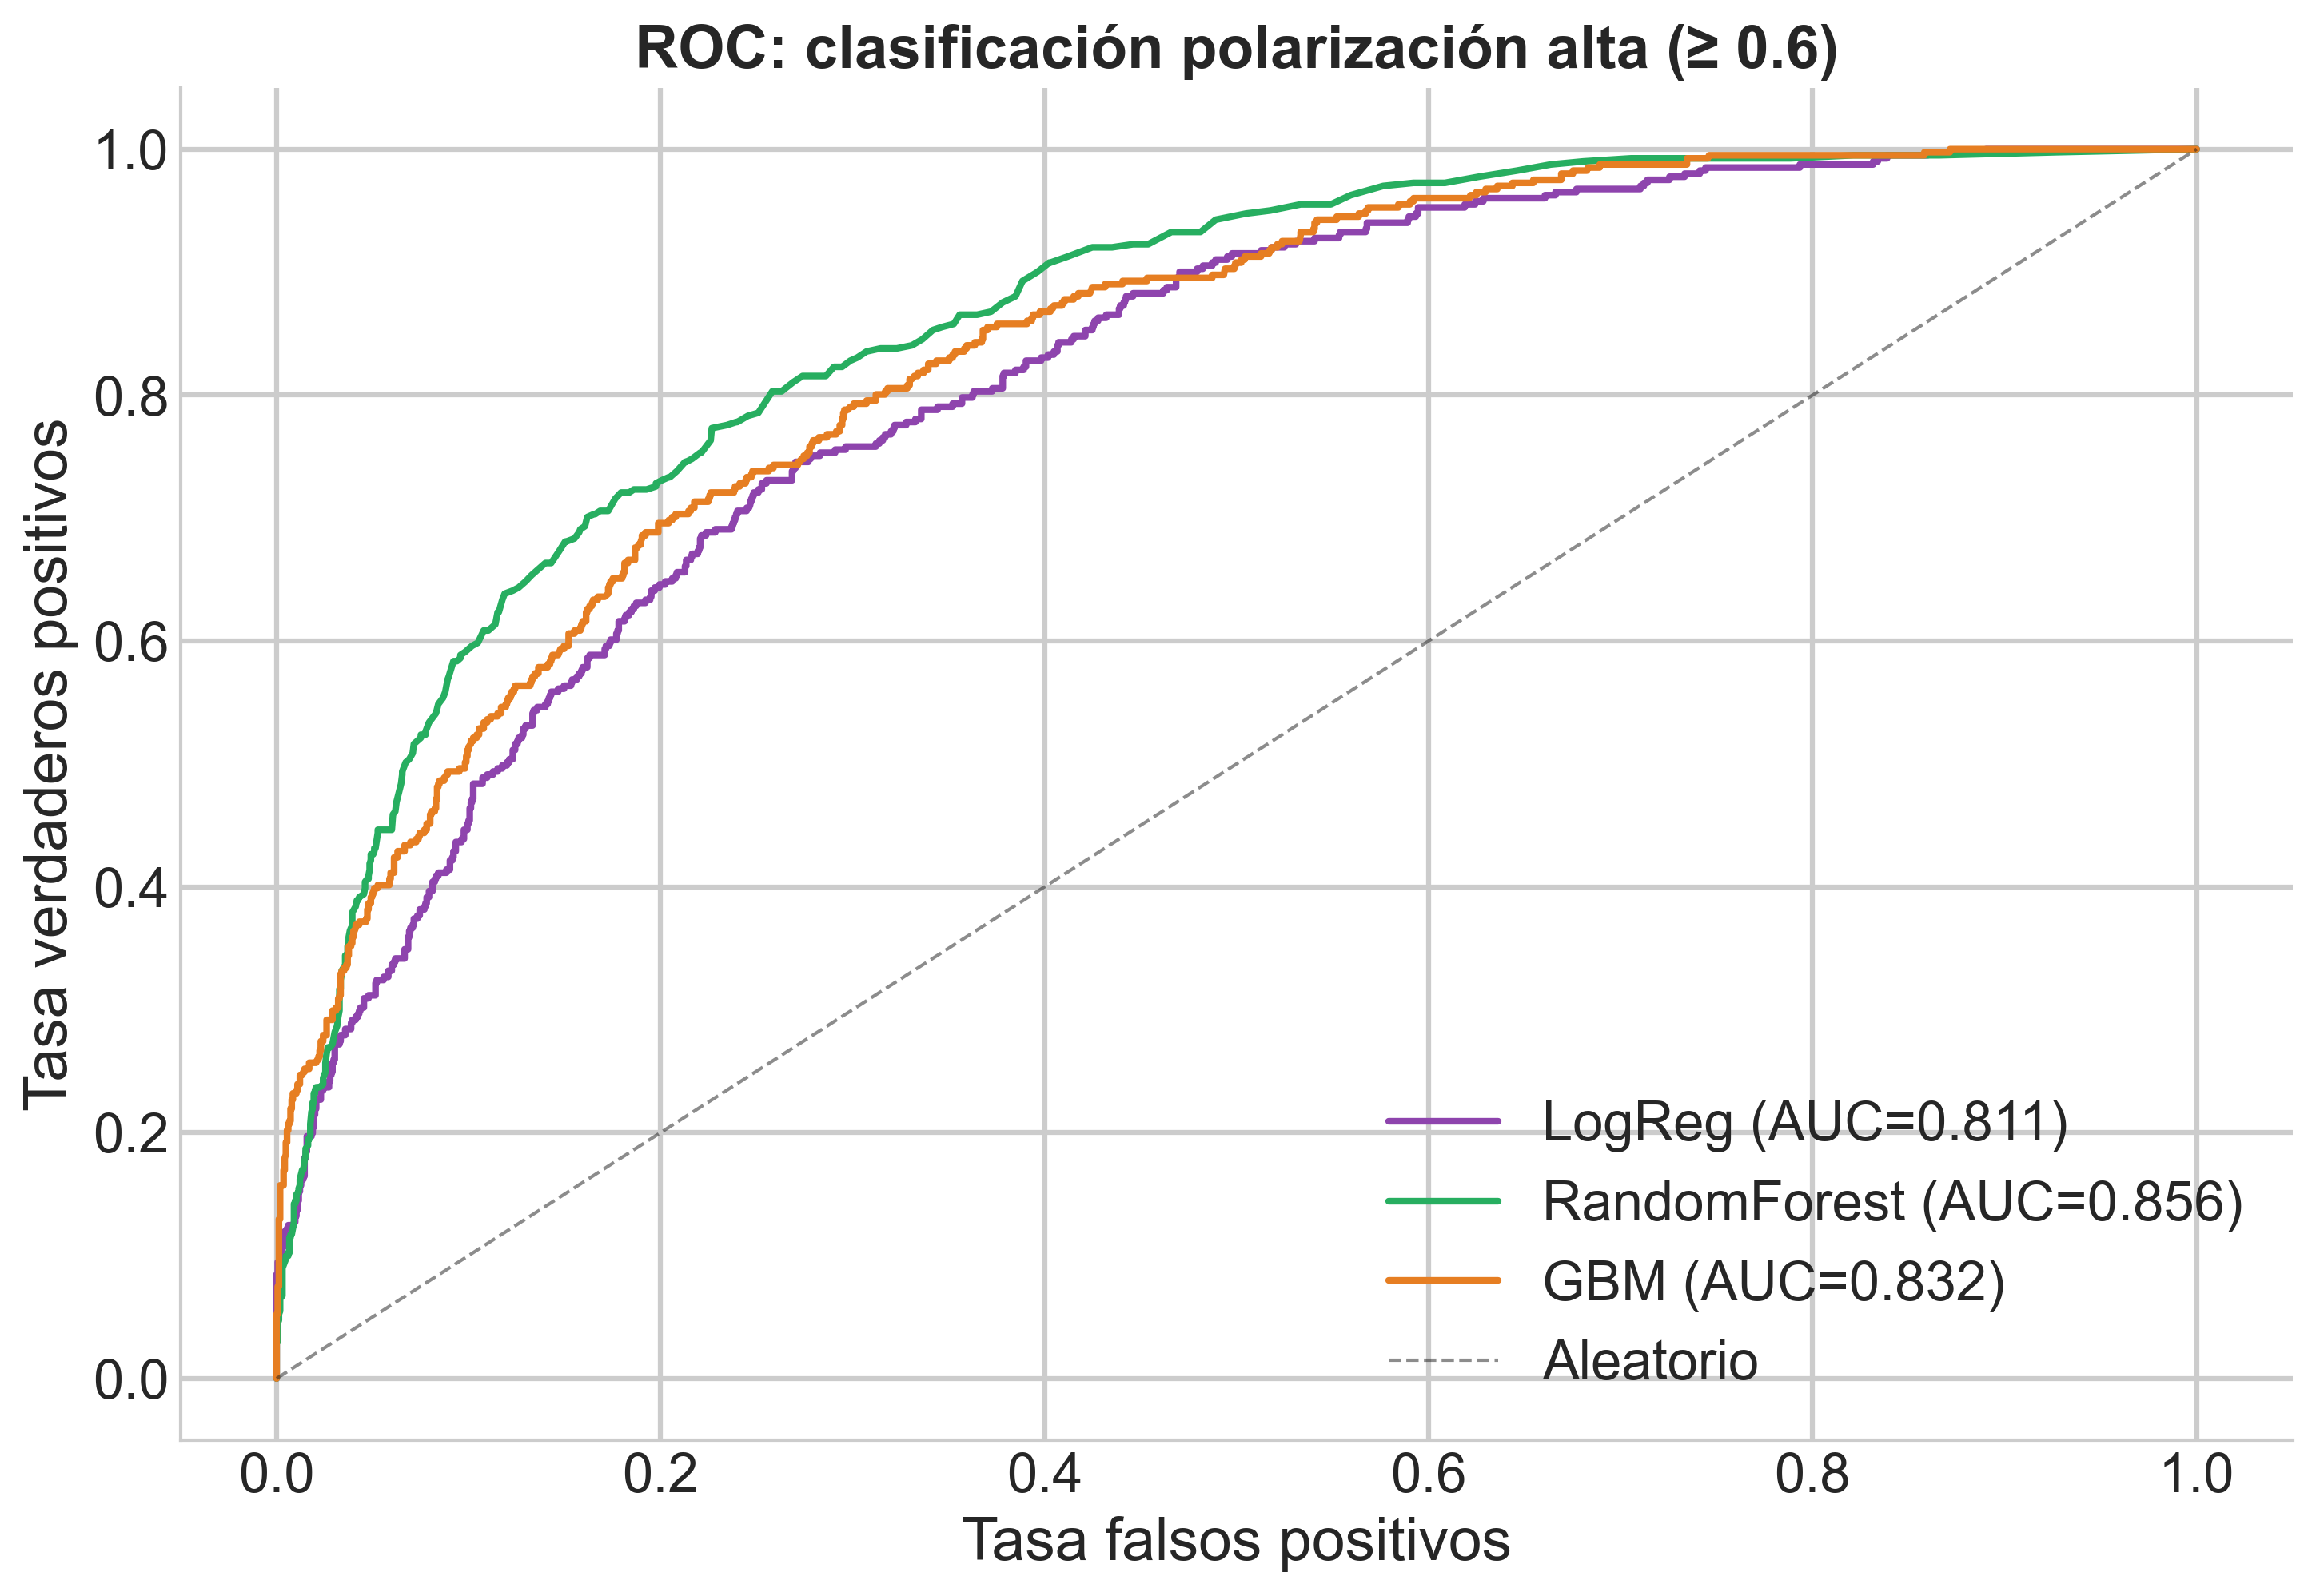
\includegraphics[width=0.82\textwidth,height=\textheight]{fig_thesis/roc_curves_polarizacion_alta.png}

}

\caption{\label{fig-roc}Curvas ROC para la clasificación de polarización
alta.}

\end{figure}%

\subsection{Estrategia, frontera, perfiles y
errores}\label{estrategia-frontera-perfiles-y-errores}

Las tablas completas de clasificación multiclase de estrategia
(Table~\ref{tbl-anexo-estrategia-resumen} y
Table~\ref{tbl-anexo-estrategia-clases}), frontera política
(Table~\ref{tbl-anexo-frontera-resumen} y
Table~\ref{tbl-anexo-frontera-clases}), perfiles K-means
(Table~\ref{tbl-anexo-perfiles-kmeans}) y análisis de errores
(Table~\ref{tbl-anexo-errores-sistematicos}) se detallan en el Anexo A.
Aquí se sintetizan los tres resultados principales.

Primero, estos resultados indican que la frontera política es
parcialmente recuperable desde texto corto y ruidoso (F1-macro = 0.725
en el mejor modelo), lo que sugiere que el concepto teórico de Mouffe
deja una huella textual detectable, aunque con las limitaciones propias
de un corpus informal y no curado.

Segundo, los perfiles K-means (K = 3) revelan que la hostilidad no se
distribuye como un continuo homogéneo, sino que se organiza en
configuraciones discursivas diferenciadas: el cluster 0 agrupa
comentarios de baja polarización con marcos diagnósticos y sin
estrategia adversarial; el cluster 1 combina deslegitimación con
desprecio en hilos sobre Jara; y el cluster 2 concentra ridiculización
con desprecio dirigida a Kast.

Tercero, el análisis de errores muestra que los falsos negativos
presentan polarización real alta (0.685) pero textos más breves que los
verdaderos positivos, delimitando las condiciones bajo las cuales el
pipeline pierde sensibilidad: comentarios hostiles pero concisos, donde
la señal discursiva es insuficiente para superar el umbral de
clasificación.

\bookmarksetup{startatroot}

\chapter{Interpretación de
Resultados}\label{interpretaciuxf3n-de-resultados}

\section{Reconfiguración del antagonismo: estrategias, marcos y
fronteras}\label{reconfiguraciuxf3n-del-antagonismo-estrategias-marcos-y-fronteras}

\subsection{Estrategias por candidato}\label{estrategias-por-candidato}

En este apartado conviene distinguir dos agregaciones: la
\textbf{frontera política} del comentario (inter-bloque, intra-bloque o
sin frontera) y el \textbf{candidato objetivo} al que se dirige el
mensaje. La Table~\ref{tbl-estrategia-frontera} cuantifica la primera:
proporción de cada estrategia discursiva según tipo de frontera. La
distribución por candidato se incluye en el Anexo A
(Figure~\ref{fig-anexo-estrategias-candidato}).

Esa lectura por frontera revela un patrón que merece atención: la lógica
del antagonismo no se distribuye homogéneamente. Las estrategias de
mayor carga adversarial --- construcción de amenaza (66.3\%
inter-bloque) y esencialización (66.0\%) --- se concentran
abrumadoramente en la confrontación entre bloques ideológicos, mientras
que la ridiculización presenta una distribución más equilibrada (48.3\%
inter, 21.9\% intra). Esto sugiere que la hostilidad no opera como un
fenómeno unitario: su forma cambia según la arquitectura del adversario
que el comentario construye. Cuando el enemigo es externo al bloque, se
recurre a estrategias que lo presentan como amenaza esencial; cuando la
disputa es interna, predomina un registro más irónico y deslegitimador.

\begin{longtable}[t]{lrrr}

\caption{\label{tbl-estrategia-frontera}Estrategias discursivas por tipo
de frontera política.}

\tabularnewline

\\
\toprule
Estrategia & Inter & Intra & Sin.frontera\\
\midrule
\cellcolor{gray!10}{Atribución oculta} & \cellcolor{gray!10}{0.548} & \cellcolor{gray!10}{0.175} & \cellcolor{gray!10}{0.277}\\
Construcción de amenaza & 0.663 & 0.101 & 0.236\\
\cellcolor{gray!10}{Deslegitimación} & \cellcolor{gray!10}{0.578} & \cellcolor{gray!10}{0.183} & \cellcolor{gray!10}{0.239}\\
Esencialización & 0.660 & 0.111 & 0.229\\
\cellcolor{gray!10}{Ninguna} & \cellcolor{gray!10}{0.329} & \cellcolor{gray!10}{0.130} & \cellcolor{gray!10}{0.540}\\
\addlinespace
Ridiculización & 0.483 & 0.219 & 0.298\\
\bottomrule

\end{longtable}

\section{Combinaciones discursivas y dinámica
temporal}\label{combinaciones-discursivas-y-dinuxe1mica-temporal}

\subsection{Marco × emoción}\label{marco-emociuxf3n}

Las combinaciones entre marco y emoción (valores numéricos en el Anexo
A, Table~\ref{tbl-anexo-marco-emocion-top}; visualización en
Figure~\ref{fig-marco-emocion}) permiten ir más allá de las
distribuciones marginales y observar cómo se acoplan ambas dimensiones.
No toda emoción hostil se acopla del mismo modo al conflicto. Las
combinaciones más frecuentes --- conflicto + desprecio (n = 945) y
diagnóstico + indignación (n = 844) --- presentan niveles de
polarización moderados (0.46 y 0.43 respectivamente). En cambio,
combinaciones menos frecuentes como moral + desprecio (n = 702, pol. =
0.541) y otro + desprecio (n = 528, pol. = 0.544) empujan la
polarización a niveles notablemente más altos. Este patrón sugiere que
el desprecio acoplado a marcos morales constituye una configuración
discursiva particularmente hostil, más que el conflicto explícito por sí
solo.

\begin{figure}[H]

\centering{

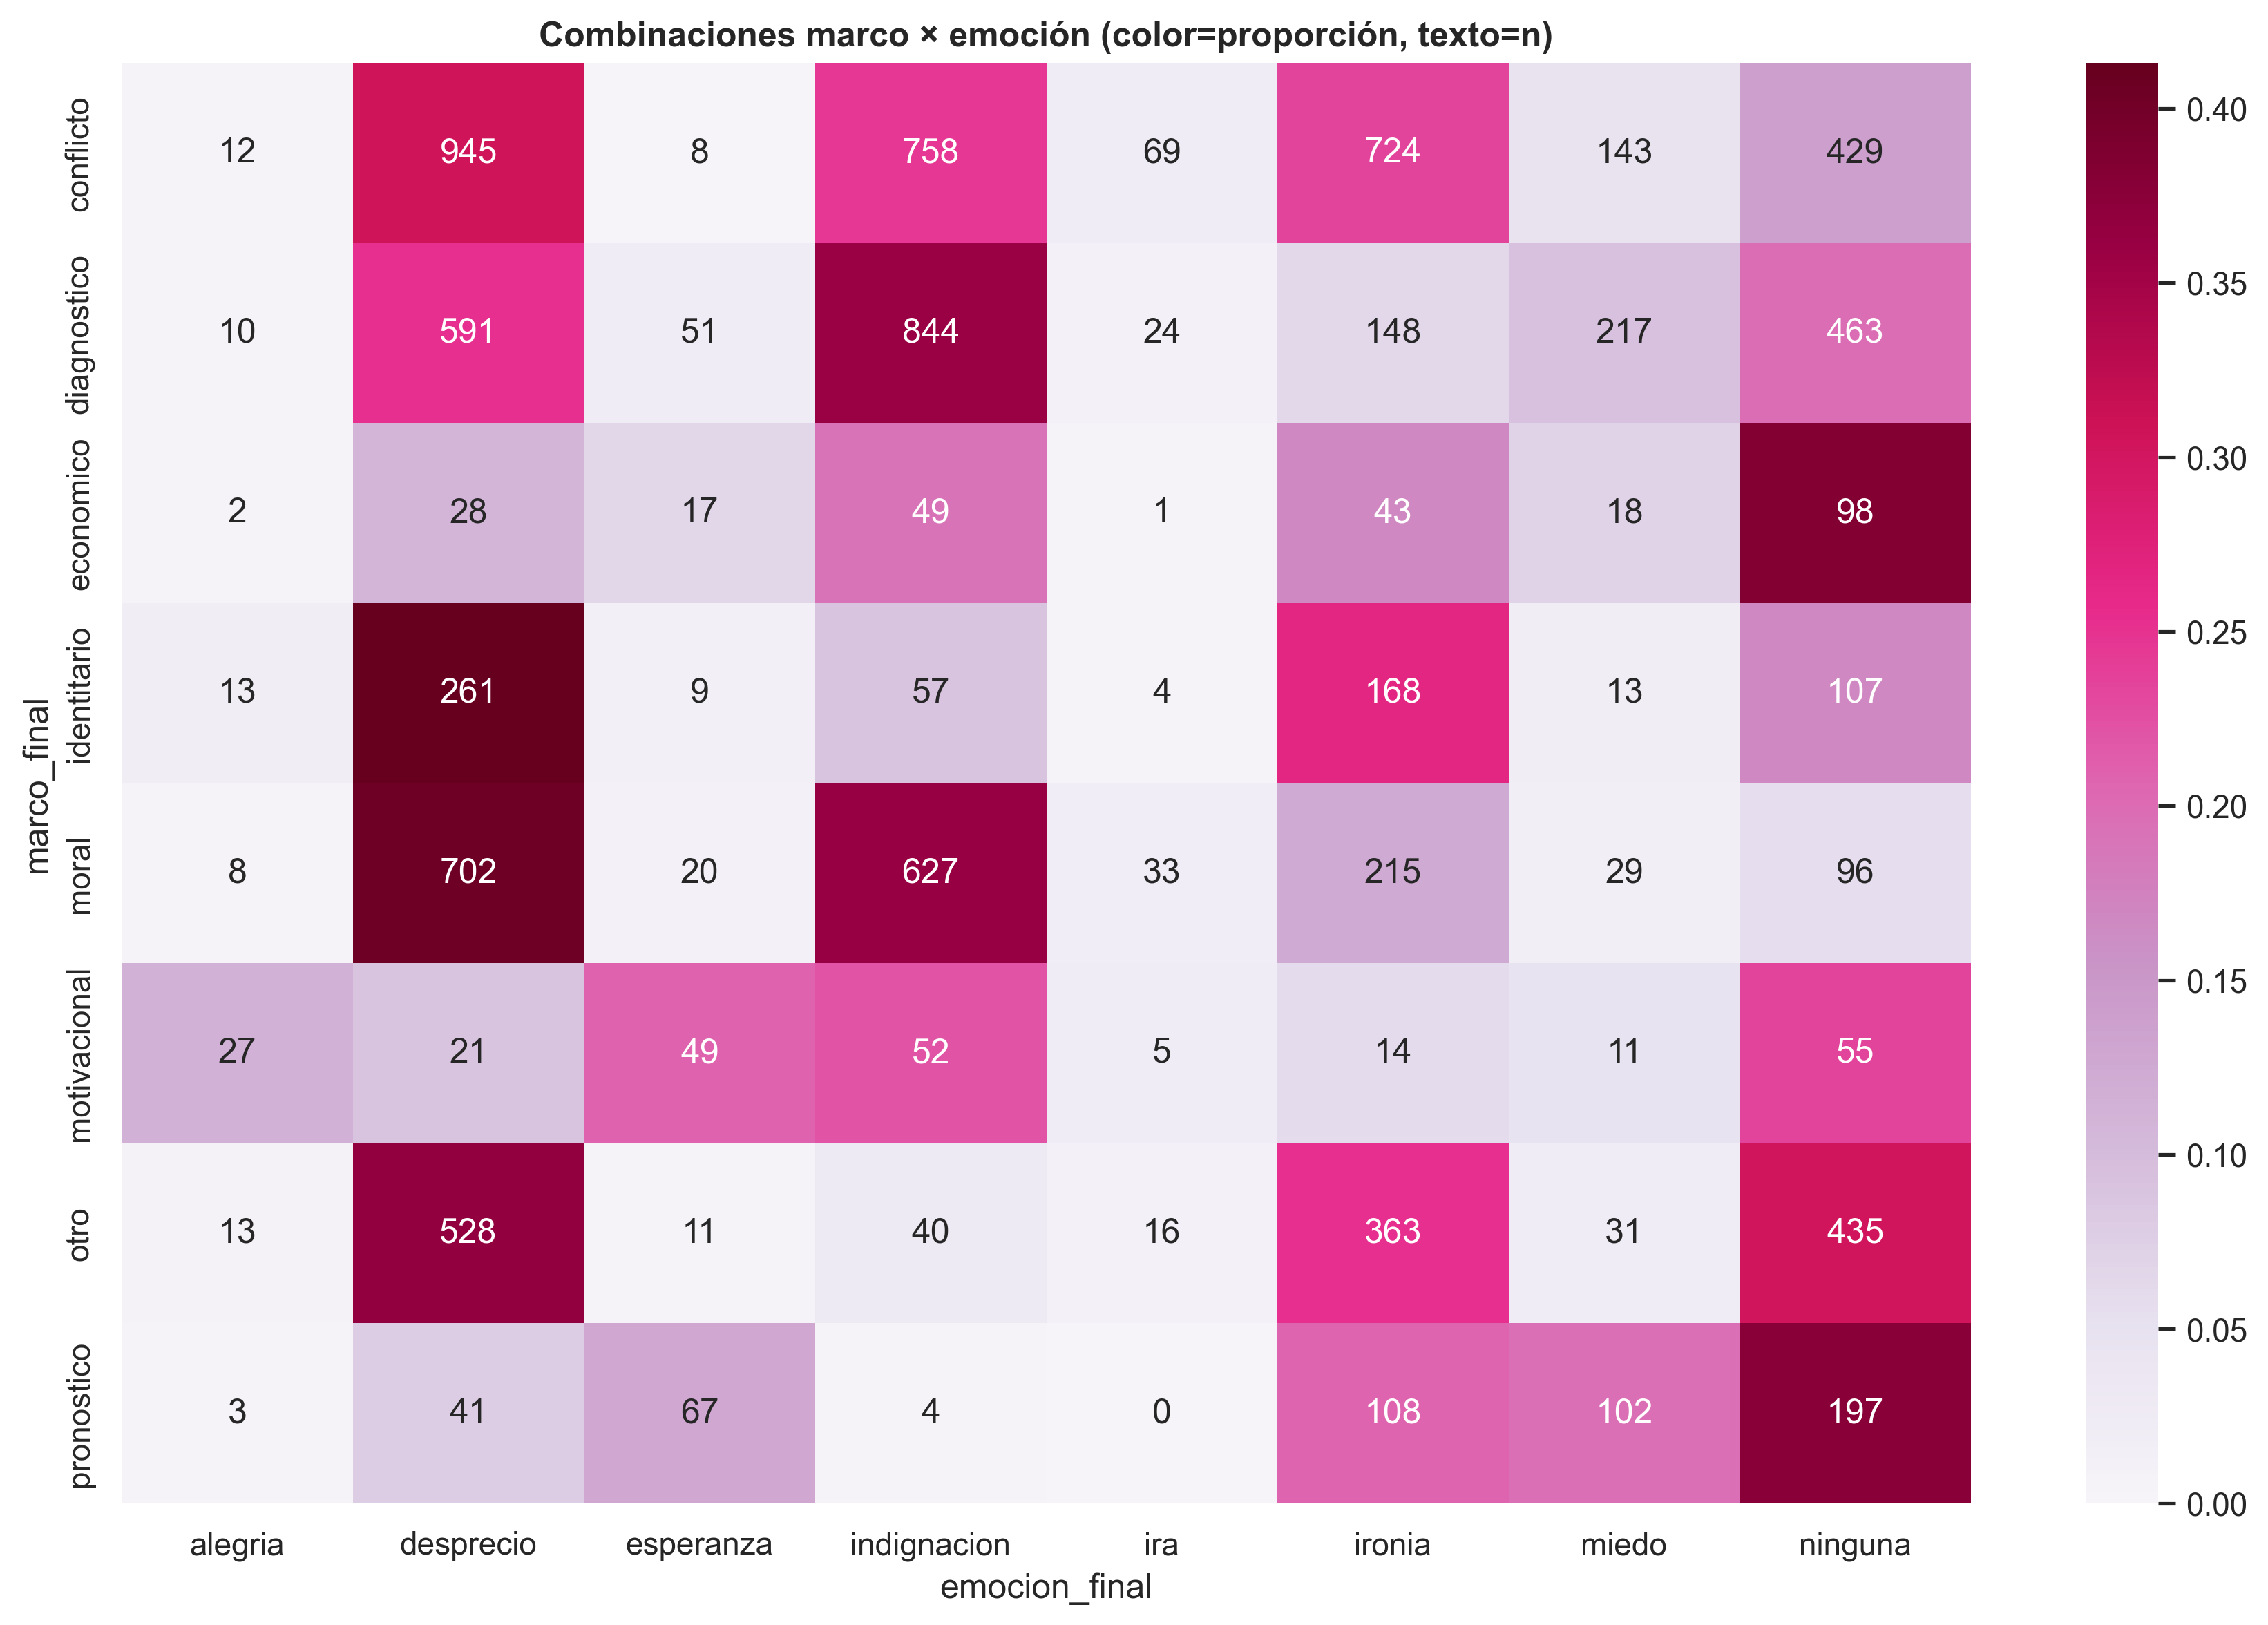
\includegraphics[width=0.82\textwidth,height=\textheight]{fig_thesis/combinaciones_marco_emocion.png}

}

\caption{\label{fig-marco-emocion}Combinaciones marco × emoción.}

\end{figure}%

\subsection{Estrategias en el tiempo}\label{estrategias-en-el-tiempo}

La serie temporal de estrategias (Figure~\ref{fig-estrategias-temporal})
permite observar si la arquitectura del adversario cambia en momentos
electorales clave. La deslegitimación se mantiene como la estrategia más
estable durante todo el ciclo, lo que sugiere un repertorio adversarial
de base que no responde a la coyuntura. La ridiculización, en cambio,
presenta mayor variabilidad y un peak notable antes de primera vuelta,
consistente con un uso más reactivo y oportunista vinculado a la
dinámica de campaña. En este punto interesa menos la fluctuación semanal
y más la dirección general: la estructura adversarial del debate se
mantiene fundamentalmente estable, con ajustes tácticos más que
transformaciones de fondo.

\begin{figure}[H]

\centering{

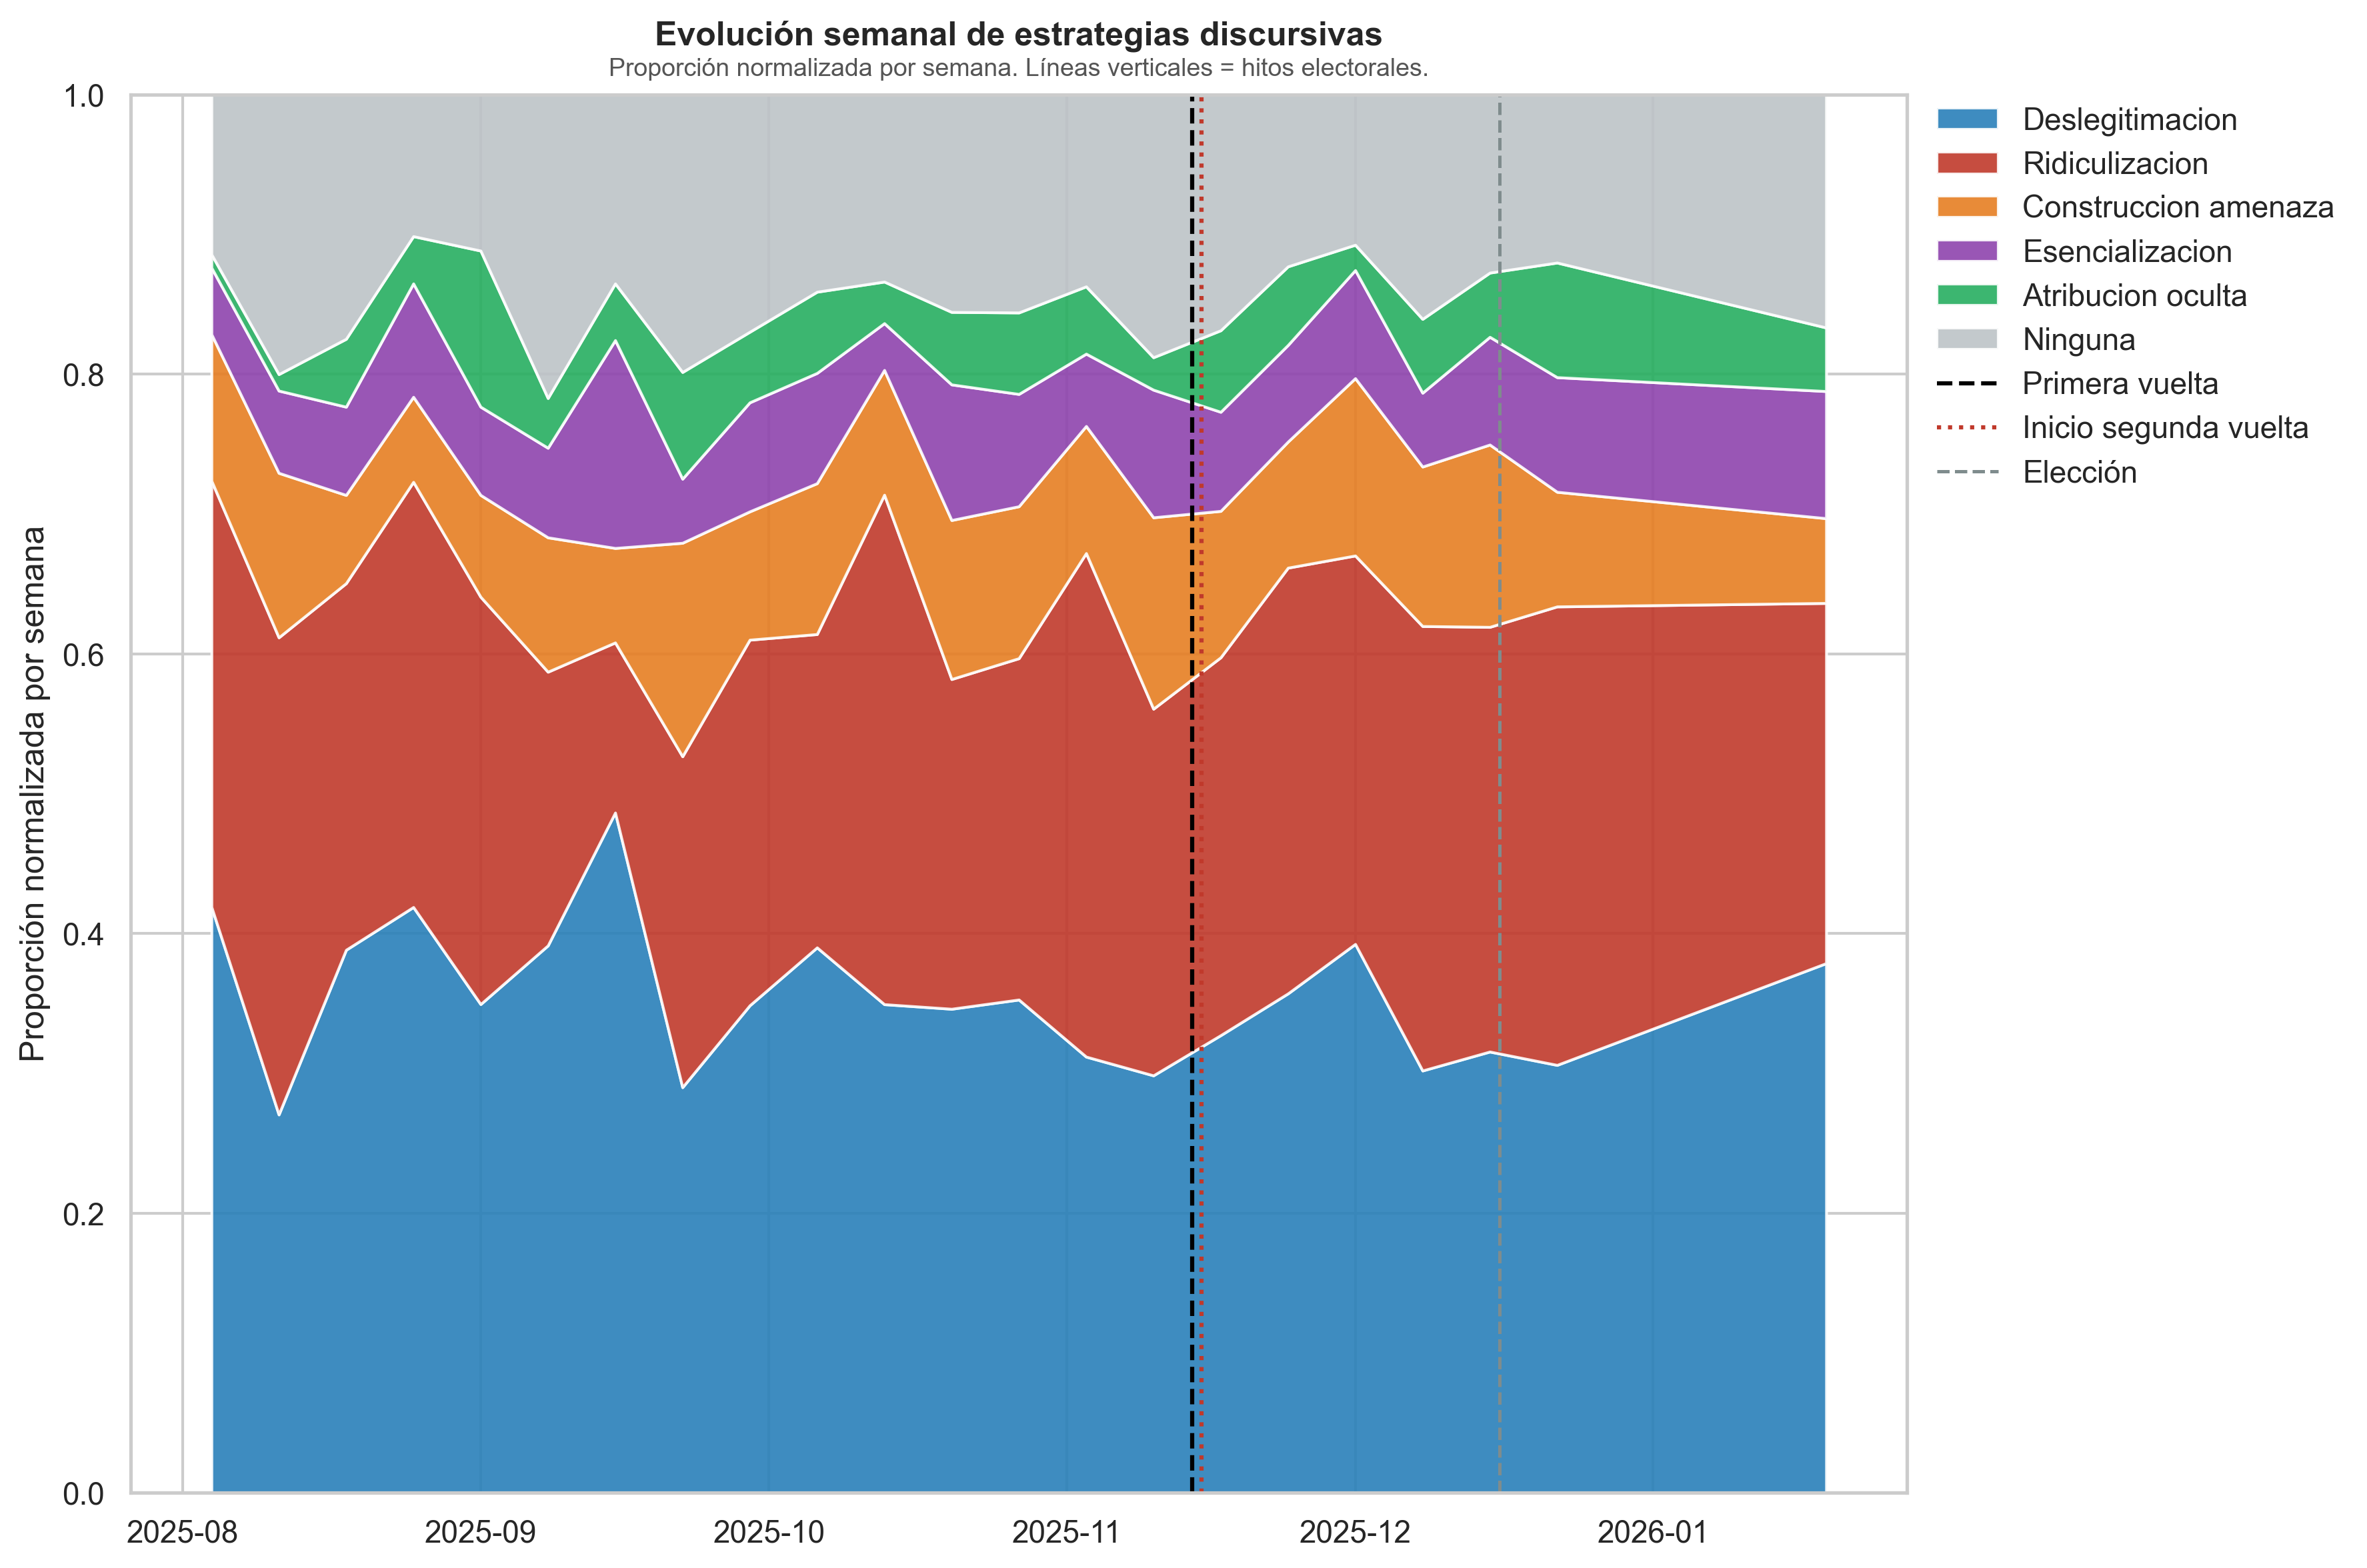
\includegraphics[width=1\textwidth,height=\textheight]{fig_thesis/serie_estrategias_semanal_mejorada.png}

}

\caption{\label{fig-estrategias-temporal}Evolución semanal de
estrategias discursivas.}

\end{figure}%

\section{Autores, persistencia y estructura del
conflicto}\label{autores-persistencia-y-estructura-del-conflicto}

\subsection{Persistencia de negatividad hacia
Kast}\label{persistencia-de-negatividad-hacia-kast}

El análisis de autores introduce una dimensión que los modelos de texto
no capturan: la estabilidad temporal de las posiciones individuales. De
los 215 autores inicialmente negativos hacia Kast, 188 (87.4\%)
mantienen esa posición a lo largo de todo el ciclo electoral. Solo 6
transitan hacia un tono positivo (2.8\%) y 21 hacia neutralidad (9.8\%).
Este nivel de persistencia indica cristalización actitudinal más que
escalamiento reactivo: la negatividad hacia Kast no se construye
progresivamente durante la campaña, sino que se presenta como una
disposición previa que el ciclo electoral refuerza pero no origina. La
tabla con la distribución porcentual completa figura en el Anexo A
(Table~\ref{tbl-anexo-kast-transiciones}).

\subsection{Cruces de tono entre candidatos (posicionamiento → segunda
vuelta hacia Kast o
Jara)}\label{cruces-de-tono-entre-candidatos-posicionamiento-segunda-vuelta-hacia-kast-o-jara}

En la segunda vuelta solo compiten Kast y Jara, por lo que el destino
del cruce es siempre el tono hacia uno de ellos en esa fase. La tabla de
cruces de tono (sin neutro) figura en el Anexo A
(Table~\ref{tbl-anexo-cruce-sentimiento-pares-sv}). La tabla de cruces
emocionales figura en el Anexo A
(Table~\ref{tbl-anexo-cruce-emocion-sin-se-pares-sv}). La
Figure~\ref{fig-alluvial-emocion-sv} resume los flujos en formato
diagrama.

\begin{figure}[H]

\centering{

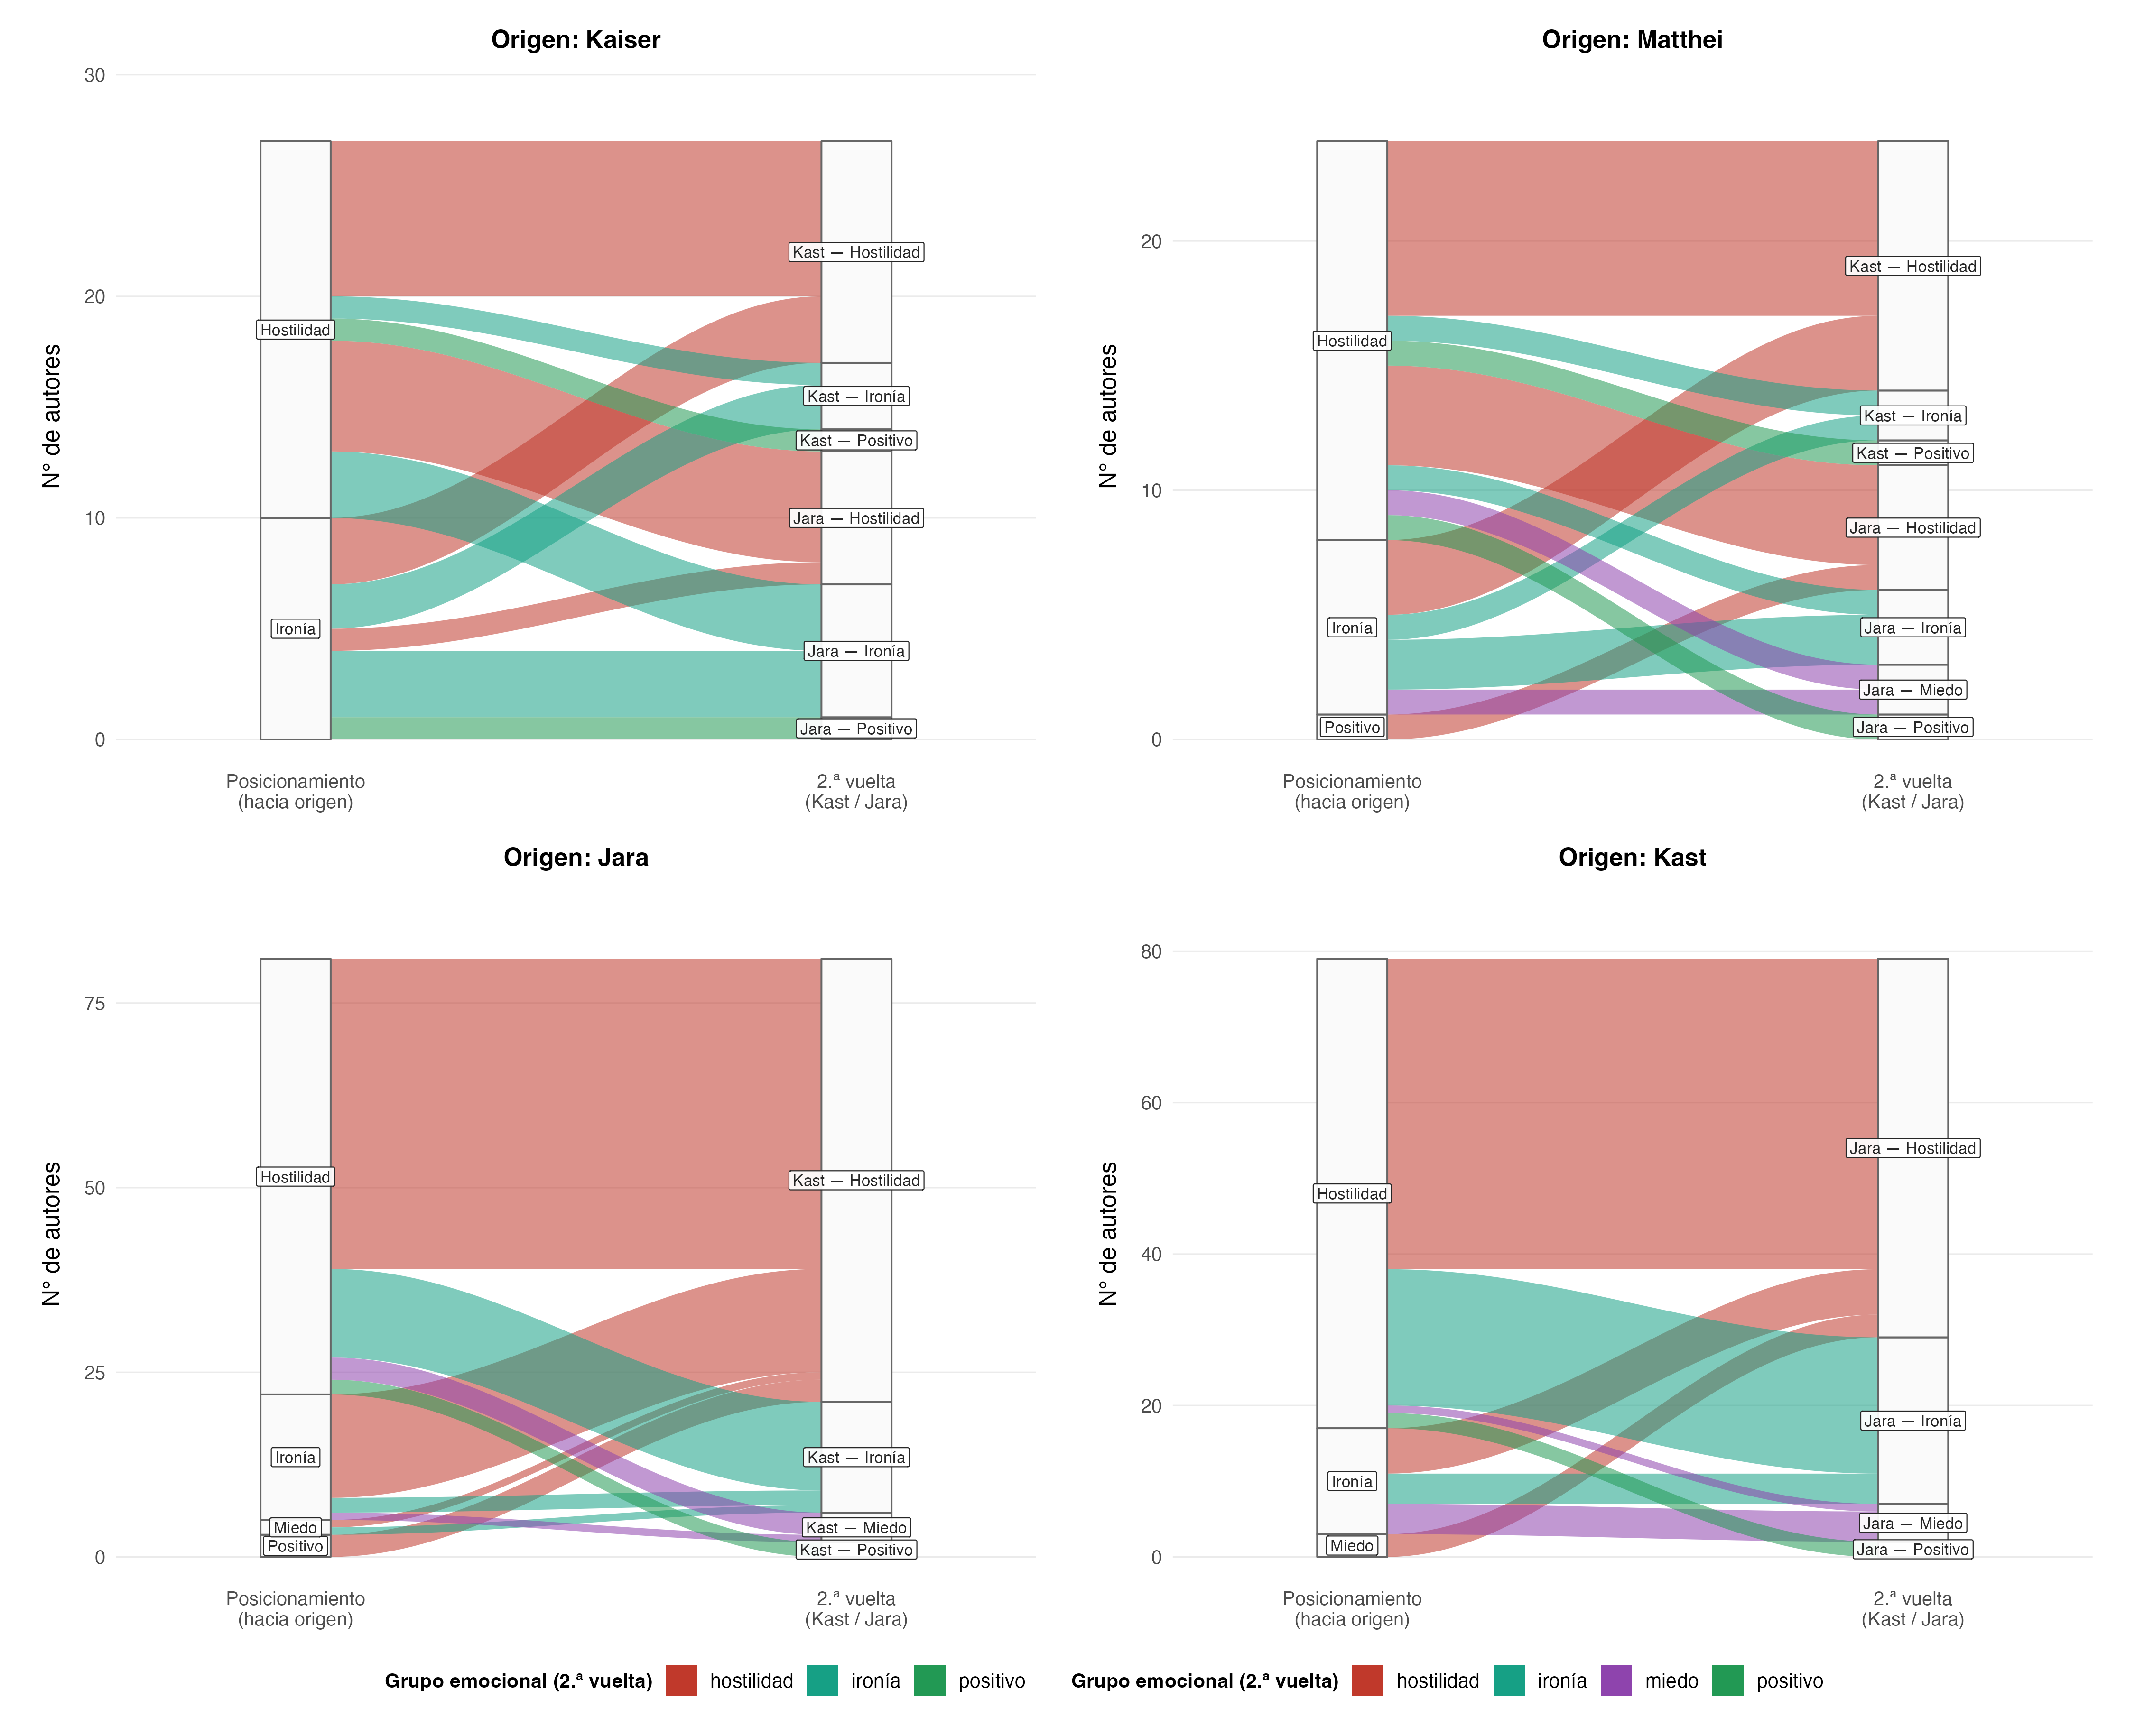
\includegraphics[width=0.92\textwidth,height=\textheight]{fig_thesis/alluvial_emocion_segunda_vuelta_por_candidato_origen_sin_sin_emocion.png}

}

\caption{\label{fig-alluvial-emocion-sv}Flujos emocionales entre
posicionamiento y segunda vuelta.}

\end{figure}%

El patrón es nítido. Los autores negativos hacia cualquier candidato en
posicionamiento permanecen negativos al transitar hacia Kast (97\% en
Jara → Kast) o hacia Jara (86--100\% según el par). Más revelador aún:
en todos los pares observados, los autores positivos hacia un candidato
se vuelven negativos al cambiar de target --- la positividad no
sobrevive al cruce adversarial. La polarización aparece así ligada al
marco del duelo electoral más que a trayectorias individuales de
simpatía.

\subsection{Actividad de autores y
polarización}\label{actividad-de-autores-y-polarizaciuxf3n}

La lectura de autores permite evaluar si la hostilidad está concentrada
en hiperactivos o distribuida en la masa de usuarios. Este punto es
teóricamente relevante porque distingue una polarización sostenida por
pocos actores intensivos de una polarización más difusa y ambiental.

La hostilidad discursiva en Reddit Chile durante la campaña presidencial
de 2025 no está concentrada en un pequeño grupo de usuarios
hiperactivos. Los autores clasificados como hiperactivos (más de 20
comentarios) presentan una polarización media similar a la de los
usuarios esporádicos, con una tendencia levemente decreciente a medida
que aumenta el número de comentarios, visible en la línea LOESS de la
Figura 8.9. Esto sugiere que la hostilidad tiene carácter ambiental y
difuso: no es producto de trolls coordinados sino de una cultura
discursiva generalizada donde la crítica hostil es el modo dominante de
participación política. Como resume la
Table~\ref{tbl-anexo-kast-transiciones}, la gran mayoría de quienes
partieron negativos \textbf{permanece} en negativo; solo una minoría
pasa a tono positivo o neutro, lo que sugiere cristalización actitudinal
más que escalamiento reactivo.

\begin{figure}[H]

\centering{


\includegraphics[width=0.82\textwidth,height=\textheight]{fig_thesis/polarizacion_por_tipo_autor.png}

}

\caption{\label{fig-autores-violin}Polarización media por tipo de
autor.}

\end{figure}%

\begin{figure}[H]

\centering{

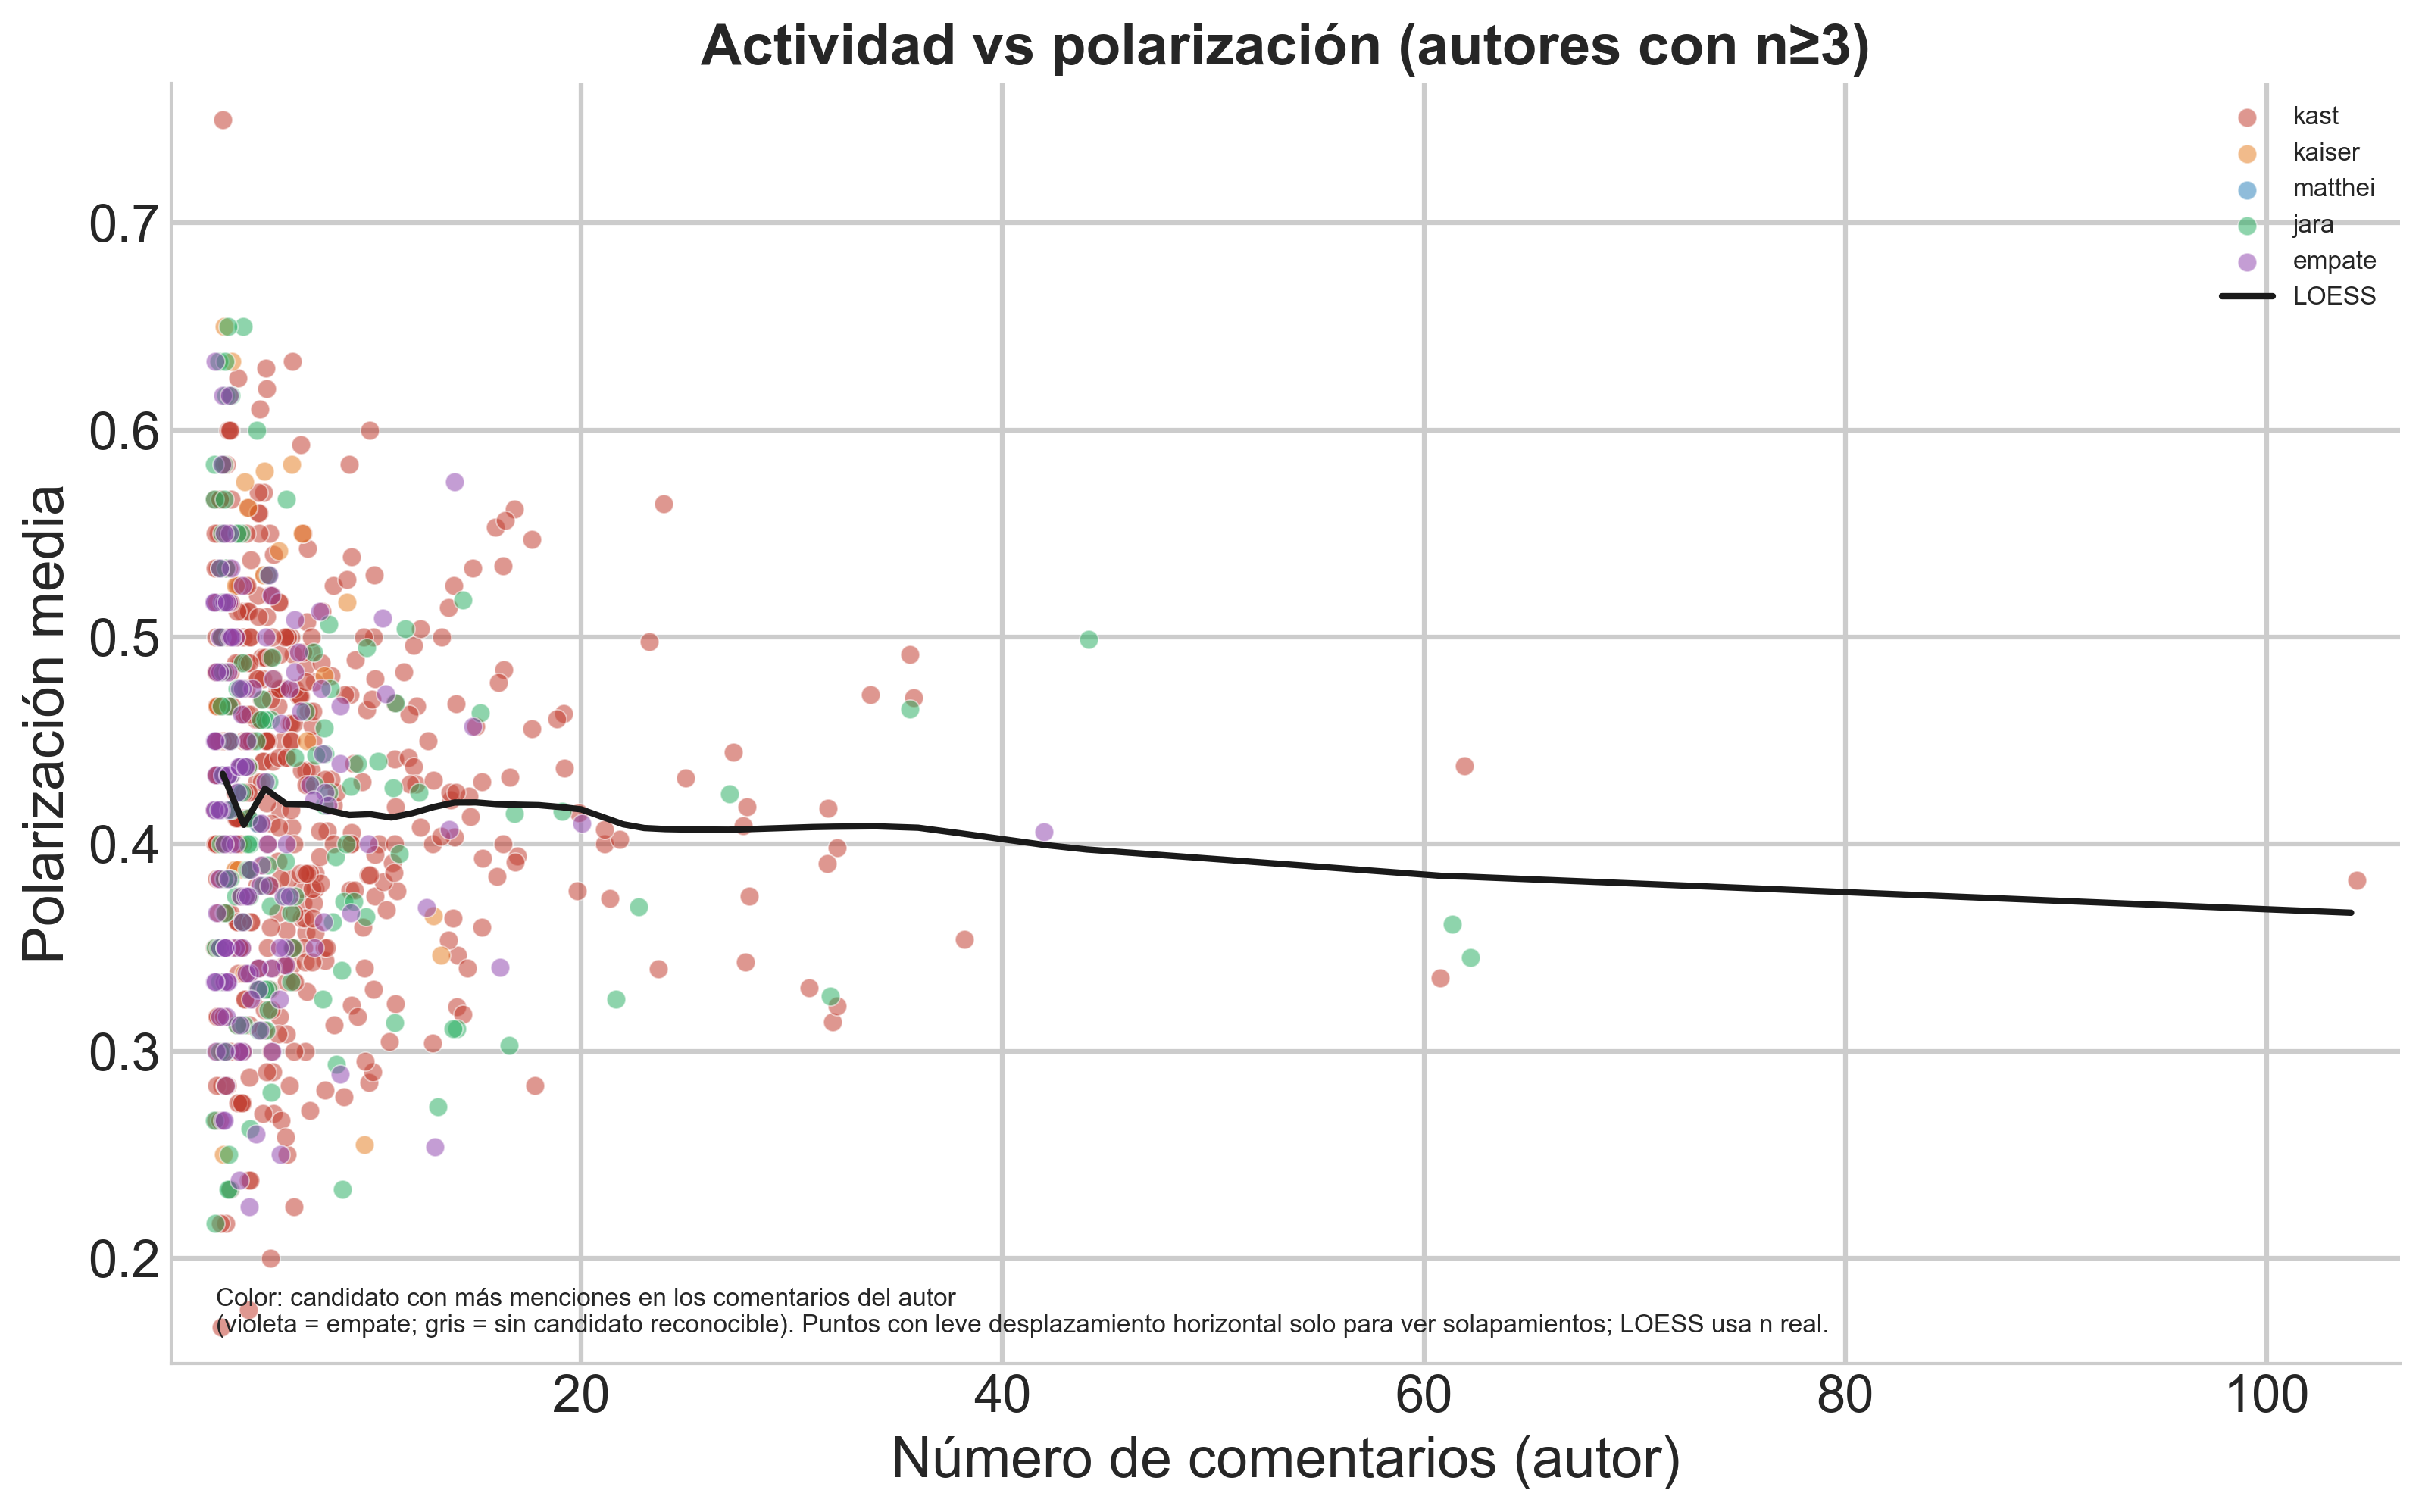
\includegraphics[width=0.82\textwidth,height=\textheight]{fig_thesis/scatter_actividad_polarizacion_autores.png}

}

\caption{\label{fig-autores-scatter}Actividad y polarización media por
autor.}

\end{figure}%

\section{Espacios semánticos
acoplados}\label{espacios-semuxe1nticos-acoplados}

El atlas (Figure~\ref{fig-3d-atlas-global-v1}) ofrece una lectura visual
que complementa los hallazgos estadísticos anteriores. El panel de
candidatos (superior derecho) muestra una superposición casi completa de
los cuatro colores: no existen regiones exclusivas por candidato. Desde
la perspectiva de Mouffe, esto sugiere que la frontera política no se
traza entre vocabularios diferenciados, sino a través de un repertorio
léxico compartido --- la polarización es una propiedad del discurso, no
del target.

El panel de emociones (inferior derecho), en cambio, presenta
agrupaciones parciales reconocibles: la ira y el desprecio ocupan zonas
distintas del espacio, indicando que se vehiculizan a través de
vocabularios diferenciados. La dimensión emocional organiza el espacio
discursivo con mayor poder que la dimensión del adversario, consistente
con la literatura sobre polarización afectiva (Iyengar, 2019).

El panel de polarización (inferior izquierdo) completa la lectura: la
hostilidad se distribuye de manera difusa a lo largo de todo el espacio,
sin concentrarse en un cluster específico. Esta dispersión constituye la
representación geométrica del hallazgo central de la tesis: la
hostilidad es ambiental, no focalizada.

\begin{figure}[H]

\centering{

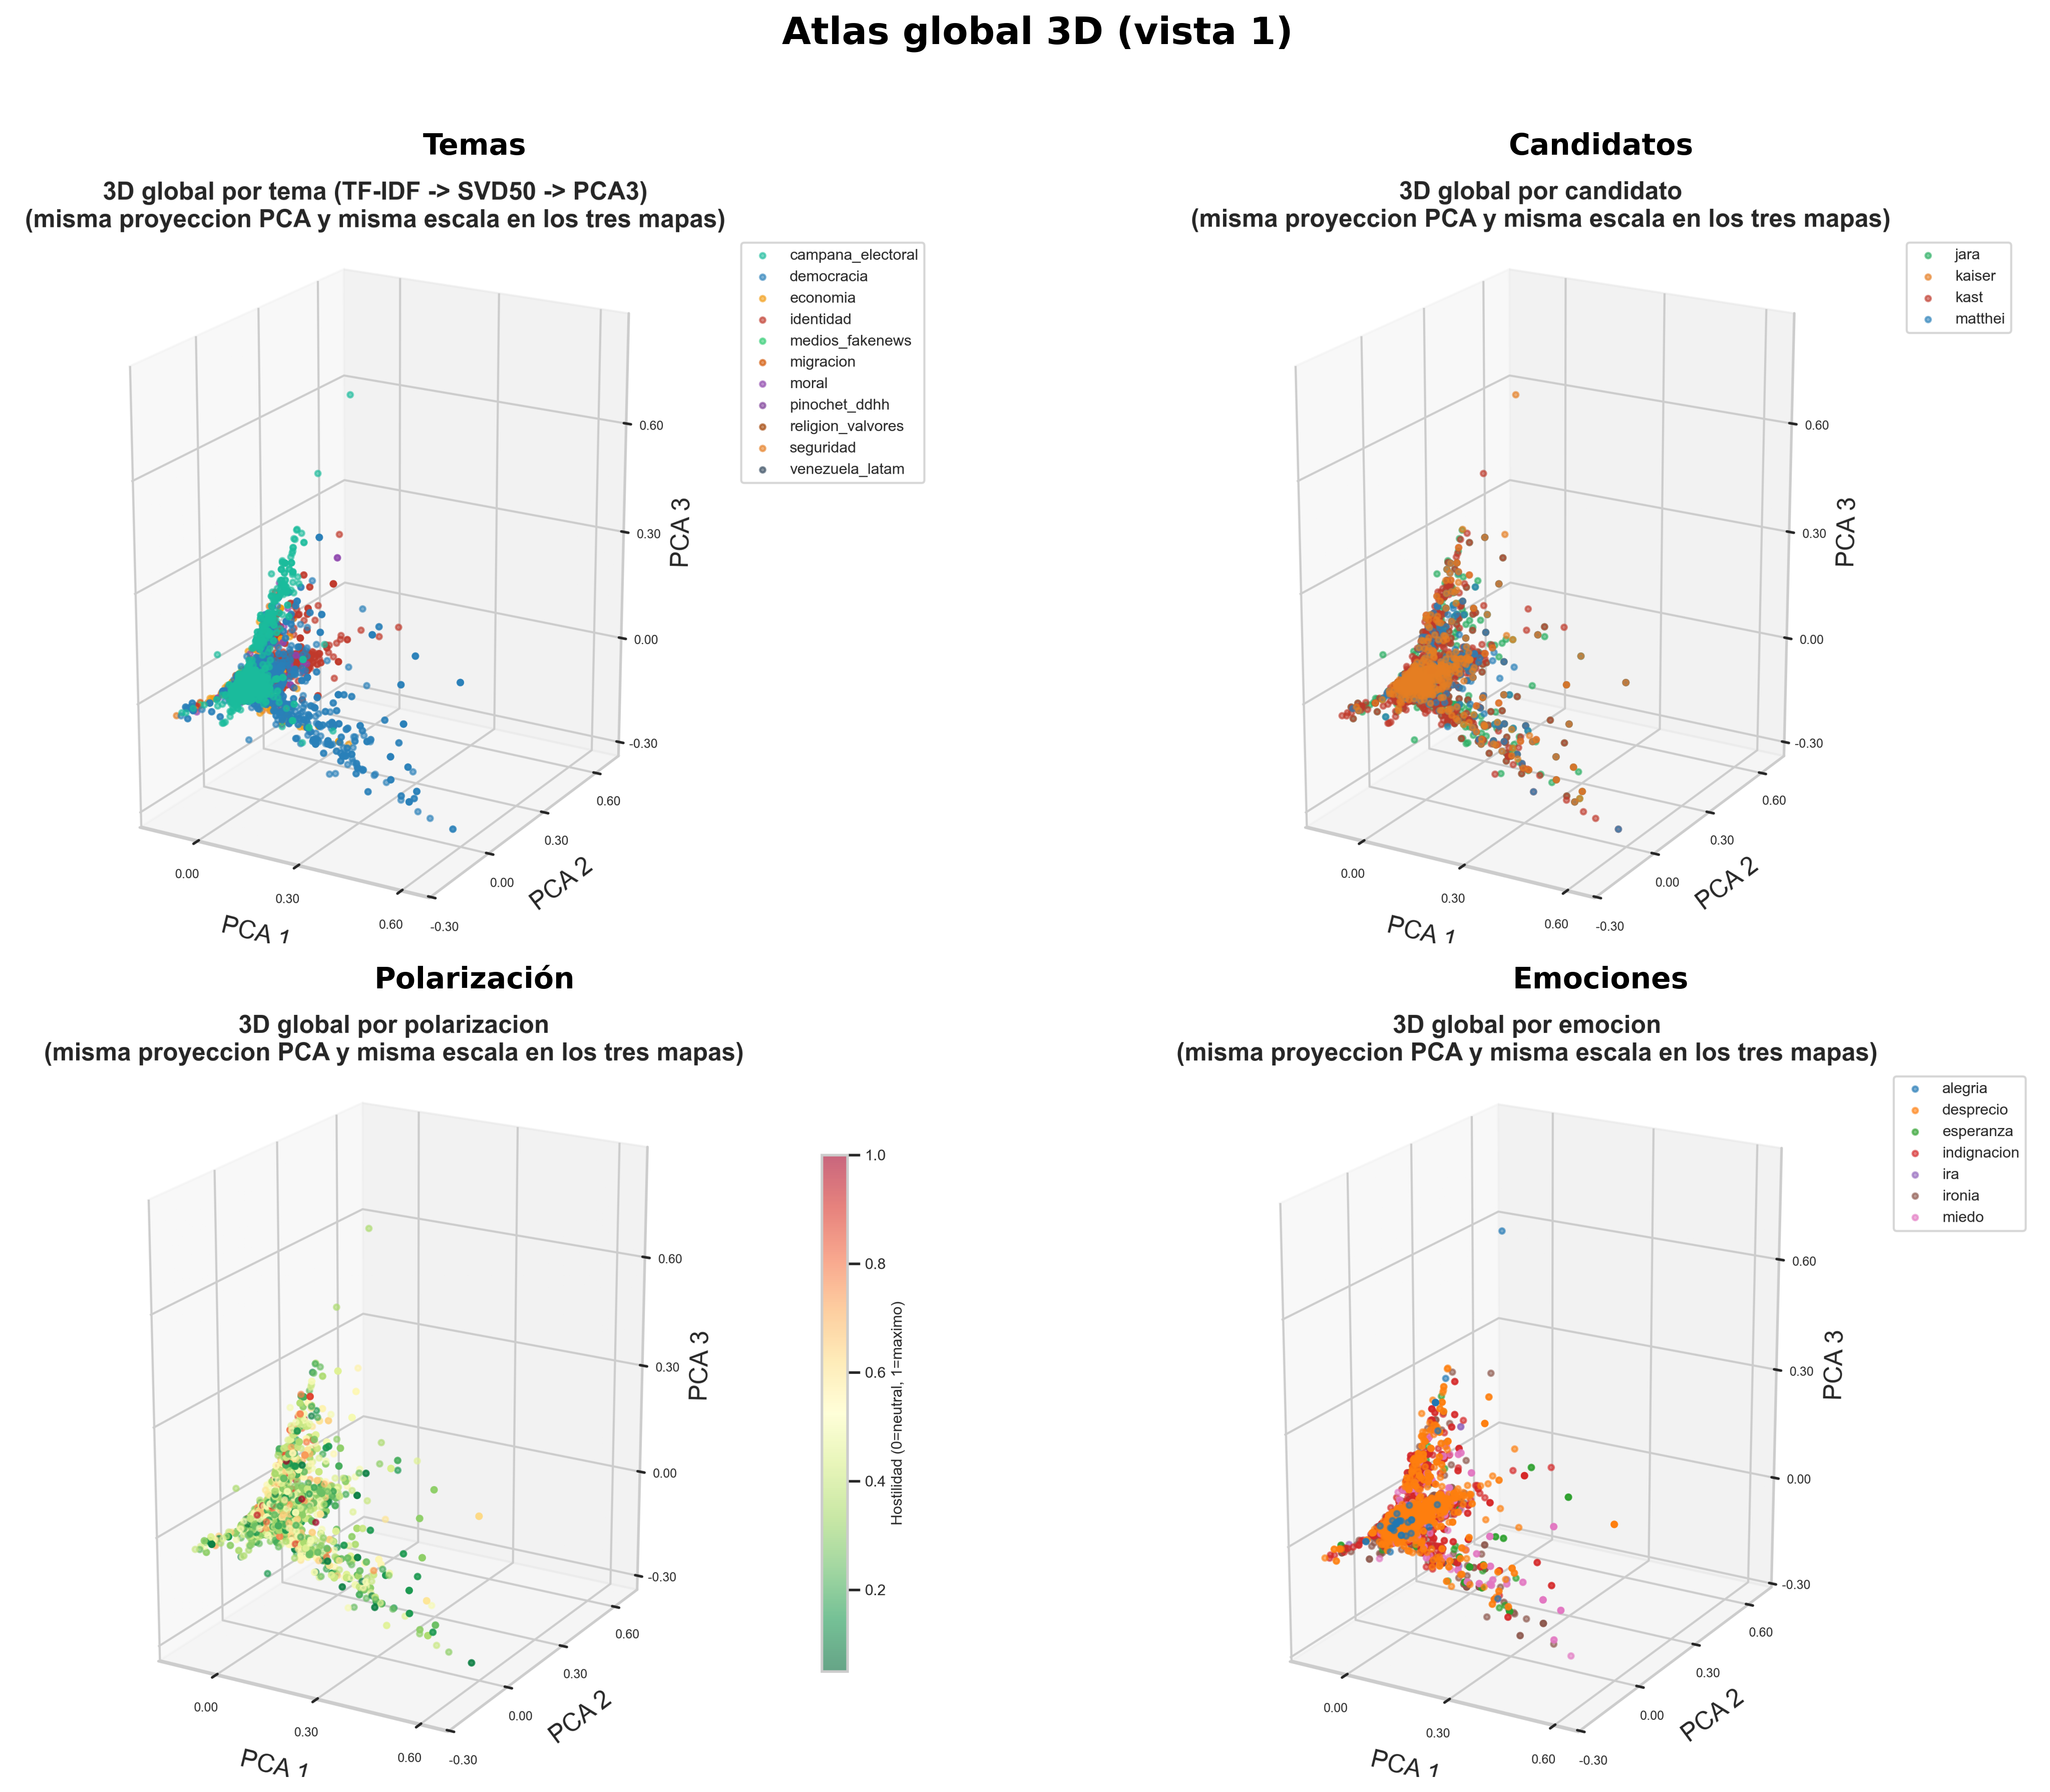
\includegraphics[width=1\textwidth,height=\textheight]{fig_thesis/3d_atlas_v1_globales.png}

}

\caption{\label{fig-3d-atlas-global-v1}Atlas global 3D: temas,
candidatos, polarización y emociones.}

\end{figure}%

\bookmarksetup{startatroot}

\chapter{Conclusión}\label{conclusiuxf3n}

\section{Síntesis de hallazgos}\label{suxedntesis-de-hallazgos}

Esta tesis se propuso analizar cómo se configura y evoluciona la
conversación política en Reddit durante la campaña presidencial chilena
de 2025, con énfasis en la reconfiguración del antagonismo dentro del
campo de las derechas. Los hallazgos pueden organizarse en tres planos:
metodológico, sustantivo y teórico.

En el plano metodológico, el sistema de doble clasificación automática
(OpenAI y DeepSeek) demostró que las variables discursivas estructuradas
--- marco, emoción, estrategia y frontera --- aportan varianza propia
sobre la polarización (R² = +0.187 respecto del texto puro en el modelo
combinado) y no constituyen una mera recodificación del contenido
léxico. Este resultado justifica el uso de LLMs como instrumentos de
medición discursiva, siempre que se acompañen de validación inter-modelo
y se expliciten las dimensiones donde el acuerdo es bajo (emoción: κ =
0.076; marco: κ = 0.136). El modelo de desacuerdo mostró además que la
discrepancia entre anotadores es parcialmente predecible (accuracy =
0.680) y se concentra en comentarios breves, irónicos o con baja
densidad de marcadores explícitos, lo que permite anticipar las
condiciones de menor fiabilidad del pipeline.

En el plano sustantivo, cinco hallazgos articulan la lectura empírica.
Primero, el candidato como target no predice la polarización (β ≈ 0, p =
0.818 en el OLS; última posición en importancia por permutación),
mientras que la ira (β = 0.369), las estrategias adversariales y el tipo
de hilo sí lo hacen. La hostilidad se explica por el \emph{cómo} del
discurso, no por el \emph{quién} es atacado. Segundo, la frontera
política es computacionalmente recuperable desde texto corto y ruidoso
(F1-macro = 0.725), operacionalizando un concepto teórico que hasta
ahora carecía de medición empírica en corpus informales. Tercero, el
84\% del corpus adversarial se organiza en tres perfiles discursivos
diferenciados --- deslegitimación con desprecio, ridiculización con
desprecio e interacción de baja hostilidad con marcos diagnósticos ---
lo que indica que la polarización no es un continuo homogéneo sino una
ecología de configuraciones. Cuarto, el 87.4\% de los autores
inicialmente negativos hacia Kast mantiene esa posición durante todo el
ciclo electoral, con solo un 2.8\% de transición hacia positividad,
sugiriendo cristalización actitudinal más que escalamiento reactivo.
Quinto, los cruces de tono entre candidatos muestran que la positividad
no sobrevive al cambio de target adversarial: en todos los pares
observados, los autores positivos hacia un candidato se vuelven
negativos al transitar hacia el adversario de segunda vuelta.

En el plano teórico, estos hallazgos convergen en una tesis central: la
polarización discursiva en Reddit Chile es ambiental, no focalizada;
estructural, no episódica; y se organiza más por la dimensión emocional
que por el target político.

\section{Implicaciones teóricas}\label{implicaciones-teuxf3ricas}

Los resultados dialogan con tres cuerpos de literatura.

Respecto de la polarización afectiva, la evidencia muestra que la
hostilidad no está concentrada en un grupo de usuarios hiperactivos ni
se escala progresivamente durante la campaña: tiene un carácter difuso y
cristalizado. Esto es consistente con la noción de Iyengar (2019) de que
la polarización afectiva opera como disposición previa más que como
respuesta coyuntural, y la extiende al contexto latinoamericano digital,
donde la evidencia empírica es aún escasa. La persistencia del 87.4\%
hacia Kast y la convergencia adversarial desde todos los candidatos de
origen sugieren que Reddit Chile funciona como un espacio donde las
disposiciones negativas se refuerzan mutuamente más que donde se
originan.

Respecto de Mouffe y la frontera política, el hallazgo de que la
frontera es computacionalmente detectable (F1 = 0.725) constituye, hasta
donde se ha podido verificar, una de las primeras operacionalizaciones
cuantitativas del concepto en texto digital informal. Más relevante aún
es que el antagonismo no depende del candidato sino de la configuración
discursiva: los mismos recursos léxicos se despliegan contra distintos
adversarios, y el atlas 3D confirma que el espacio semántico se organiza
por emoción y tema antes que por target. Esto sugiere que la frontera
política mouffiana no es un límite entre vocabularios, sino un modo de
articulación discursiva que atraviesa el repertorio compartido.

Respecto de la reconfiguración de las derechas chilenas, los datos
muestran que la competencia intra-bloque se expresa mediante estrategias
y marcos diferenciados --- ridiculización e ironía prevalecen en la
disputa interna, mientras que amenaza y esencialización se concentran en
la confrontación inter-bloque ---, pero que estas diferencias se
subordinan a una convergencia adversarial frente a Jara y la izquierda.
El título de esta tesis --- \emph{derecha fragmentada y un enemigo
compartido} --- se sostiene empíricamente: la fragmentación es
estratégica, la convergencia es emocional.

\section{Implicaciones prácticas}\label{implicaciones-pruxe1cticas}

Los hallazgos sugieren dos líneas de aplicación. En moderación de
plataformas, la priorización de intervenciones por estrategia discursiva
y tipo de hilo --- más que por volumen de publicaciones o identidad de
usuarios --- podría ser más eficaz para reducir la hostilidad, dado que
el tipo de hilo es el predictor más importante del modelo (caída de R² ≈
0.50 al permutarlo). La detección automática de frontera política,
viable con los niveles de F1 observados, permitiría distinguir entre
confrontación inter-bloque e intra-bloque y adaptar las respuestas de
moderación en consecuencia.

En comunicación política, los resultados sugieren que intervenciones
orientadas a modificar el encuadre (marcos diagnósticos en lugar de
marcos de conflicto) y a desplazar emociones (indignación argumentada en
lugar de desprecio) podrían atenuar los niveles de polarización sin
suprimir el debate. La evidencia de que los hilos mixtos presentan
coeficientes negativos en el OLS indica que la exposición a posiciones
cruzadas no necesariamente escala la hostilidad, sino que puede
moderarla.

\section{Limitaciones}\label{limitaciones}

Esta investigación presenta limitaciones que deben considerarse al
interpretar los hallazgos.

En primer lugar, Reddit no es representativo de la opinión pública
chilena. Sus usuarios tienden a ser más jóvenes, masculinos, urbanos y
politizados que la población general. Los patrones documentados refieren
a la cultura discursiva de esta plataforma específica y no son
generalizables sin replicación en otros contextos. La ausencia de datos
demográficos verificables impide controlar por variables
socioestructurales que podrían mediar la relación entre discurso y
polarización.

En segundo lugar, el acuerdo inter-modelo en las dimensiones categóricas
es bajo, particularmente en emoción (κ = 0.076) y marco (κ = 0.136). Si
bien el sistema de desempate por consenso (v5.1) mitiga este problema y
el capítulo 7 demuestra que estas variables aportan varianza predictiva
no redundante, las clasificaciones individuales en estas dimensiones
deben interpretarse como aproximaciones probabilísticas, no como
mediciones de alta precisión. La validación humana (40 comentarios,
kappas reportados) es limitada en escala y no permite estimar con
certeza el sesgo sistemático de los modelos.

En tercer lugar, la atribución ideológica de los usuarios es inferida a
partir de su comportamiento discursivo, no de autodeclaraciones. Un
usuario clasificado como ``negativo hacia Kast'' podría ser un opositor
de izquierda, un simpatizante de otra corriente de derecha decepcionado,
o un usuario que comenta negativamente por razones ajenas a la
ideología. Esta ambigüedad es inherente al análisis de datos digitales
observacionales y limita la inferencia causal.

En cuarto lugar, el diseño longitudinal captura variación temporal pero
no permite establecer causalidad. Que la deslegitimación sea estable
durante todo el ciclo no implica que sea independiente de la coyuntura;
podría ser que eventos distintos activen la misma estrategia de forma
recurrente. Un diseño con ventanas de evento más finas podría abordar
esta limitación.

\section{Futuras investigaciones}\label{futuras-investigaciones}

Los resultados abren al menos cuatro líneas de investigación futura.
Primero, la replicación en otras plataformas --- particularmente
X/Twitter, donde la estructura de interacción es radicalmente distinta
--- permitiría evaluar si los patrones observados son propiedades del
debate político chileno o artefactos de la arquitectura de Reddit.
Segundo, un análisis dinámico con ventanas móviles más finas y modelos
de series temporales podría captar cambios rápidos asociados a eventos
específicos (debates televisados, declaraciones polémicas, encuestas)
que la granularidad bisegmentada de esta tesis no resuelve. Tercero, la
extensión del pipeline a otros fenómenos discursivos --- desinformación,
coordinación inorgánica, astroturfing --- permitiría evaluar si las
mismas variables que predicen polarización también predicen otros tipos
de comportamiento hostil. Cuarto, la incorporación de modelos de
lenguaje más recientes y la ampliación de la validación humana podrían
mejorar los niveles de acuerdo en las dimensiones más débiles del
sistema de clasificación.

\section{Reflexión final}\label{reflexiuxf3n-final}

La democracia digital se juega en espacios donde la discusión pública
convive con repertorios hostiles que no son ni aleatorios ni
irracionales: tienen estructura, persistencia y lógica interna. Esta
tesis muestra que la frontera política es observable en texto digital
informal, que la hostilidad es ambiental antes que focalizada, y que las
derechas chilenas se reconfiguran en una tensión permanente entre
competencia interna y convergencia adversarial. El candidato importa
menos que el modo en que se habla de él. La emoción organiza el espacio
discursivo con mayor poder que la identidad del adversario. Y la
negatividad, una vez cristalizada, no se revierte por efecto de la
campaña.

Estas observaciones no agotan el fenómeno, pero ofrecen un punto de
partida empírico para una conversación que las ciencias sociales
computacionales recién comienzan a articular en América Latina.

\bookmarksetup{startatroot}

\chapter{Anexo A. Tablas
complementarias}\label{anexo-a.-tablas-complementarias}

Este anexo reúne las tablas detalladas del modelado supervisado y de la
interpretación discursiva que, por su extensión o número de columnas, no
cabían en el cuerpo principal (incluidas la tabla y el coefplot del
modelo OLS de polarización del capítulo 7, el listado de las diez
combinaciones marco × emoción más frecuentes del capítulo 8, y las de
cruces electorales por autor y la persistencia de tono hacia Kast). En
el PDF, las tablas anchas se \textbf{escalan al ancho de página}
(orientación vertical en todas las páginas). En el cuerpo de los
capítulos 7 y 8 se conservan solo las tablas imprescindibles para la
línea argumental; el resto se referencia desde allí.

\textbf{A.1 Modelado de datos (capítulo 7)}

\textbf{A.1.1 Desacuerdo entre anotadores}

\begin{table}

\caption{\label{tbl-anexo-desacuerdo}Modelo de desacuerdo (OA vs.~DS).}

\centering{

[!h]
\centering
\resizebox{\ifdim\width>\linewidth\linewidth\else\width\fi}{!}{
\begin{tabular}{lrr}
\toprule
modelo & accuracy & f1\_macro\\
\midrule
\cellcolor{gray!10}{LogReg} & \cellcolor{gray!10}{0.622} & \cellcolor{gray!10}{0.593}\\
LinearSVM & 0.599 & 0.561\\
\cellcolor{gray!10}{RandomForest} & \cellcolor{gray!10}{0.680} & \cellcolor{gray!10}{0.540}\\
\bottomrule
\end{tabular}}

}

\end{table}%

\textbf{A.1.2 Comparación de configuraciones de características (texto,
LLM, combinado)}

\begin{table}

\caption{\label{tbl-anexo-config-features}Comparación de configuraciones
de variables.}

\centering{

[!h]
\centering
\resizebox{\ifdim\width>\linewidth\linewidth\else\width\fi}{!}{
\begin{tabular}{lrrrrr}
\toprule
config & MAE\_mean & MAE\_sd & R2\_mean & R2\_sd & delta\_vs\_texto\\
\midrule
\cellcolor{gray!10}{A\_TF-IDF} & \cellcolor{gray!10}{0.1052} & \cellcolor{gray!10}{0.0022} & \cellcolor{gray!10}{0.4316} & \cellcolor{gray!10}{0.0272} & \cellcolor{gray!10}{0.0000}\\
B\_LLM & 0.0922 & 0.0014 & 0.5539 & 0.0095 & 0.1223\\
\cellcolor{gray!10}{C\_combinado} & \cellcolor{gray!10}{0.0842} & \cellcolor{gray!10}{0.0013} & \cellcolor{gray!10}{0.6184} & \cellcolor{gray!10}{0.0068} & \cellcolor{gray!10}{0.1868}\\
\bottomrule
\multicolumn{6}{l}{\rule{0pt}{1em}\textit{Nota.} delta\_vs\_texto: incremento de R² medio respecto de la configuración solo TF-IDF.}\\
\end{tabular}}

}

\end{table}%

\textbf{A.1.3 Calibración de probabilidades (polarización alta)}

\begin{table}

\caption{\label{tbl-anexo-calibracion}Calibración: Brier y log-loss.}

\centering{

[!h]
\centering
\resizebox{\ifdim\width>\linewidth\linewidth\else\width\fi}{!}{
\begin{tabular}{lrrrr}
\toprule
modelo & brier\_antes & brier\_despues & logloss\_antes & logloss\_despues\\
\midrule
\cellcolor{gray!10}{RandomForest} & \cellcolor{gray!10}{0.1105} & \cellcolor{gray!10}{0.1119} & \cellcolor{gray!10}{0.3654} & \cellcolor{gray!10}{0.3530}\\
GBM & 0.1138 & 0.1131 & 0.3608 & 0.3590\\
\cellcolor{gray!10}{LogReg} & \cellcolor{gray!10}{0.1780} & \cellcolor{gray!10}{0.1215} & \cellcolor{gray!10}{0.5193} & \cellcolor{gray!10}{0.4123}\\
\bottomrule
\end{tabular}}

}

\end{table}%

\textbf{A.1.4 AUC para clasificación de polarización alta}

\begin{table}

\caption{\label{tbl-anexo-auc}AUC para polarización alta.}

\centering{

[!h]
\centering
\resizebox{\ifdim\width>\linewidth\linewidth\else\width\fi}{!}{
\begin{tabular}{lr}
\toprule
modelo & AUC\\
\midrule
\cellcolor{gray!10}{LogReg} & \cellcolor{gray!10}{0.8107}\\
RandomForest & 0.8557\\
\cellcolor{gray!10}{GBM} & \cellcolor{gray!10}{0.8324}\\
\bottomrule
\end{tabular}}

}

\end{table}%

\textbf{A.1.5 Clasificación multiclase de estrategia discursiva}

\begin{table}

\caption{\label{tbl-anexo-estrategia-resumen}Estrategia (multiclase):
exactitud y F1 macro.}

\centering{

[!h]
\centering
\resizebox{\ifdim\width>\linewidth\linewidth\else\width\fi}{!}{
\begin{tabular}{lrr}
\toprule
modelo & accuracy & f1\_macro\\
\midrule
\cellcolor{gray!10}{LogReg} & \cellcolor{gray!10}{0.589} & \cellcolor{gray!10}{0.527}\\
RandomForest & 0.667 & 0.573\\
\cellcolor{gray!10}{GBM} & \cellcolor{gray!10}{0.594} & \cellcolor{gray!10}{0.452}\\
\bottomrule
\end{tabular}}

}

\end{table}%

\begin{table}

\caption{\label{tbl-anexo-estrategia-clases}Estrategia (multiclase): F1
por clase.}

\centering{

[!h]
\centering
\resizebox{\ifdim\width>\linewidth\linewidth\else\width\fi}{!}{
\begin{tabular}{llr}
\toprule
modelo & clase & f1\_clase\\
\midrule
\cellcolor{gray!10}{LogReg} & \cellcolor{gray!10}{atribucion\_oculta} & \cellcolor{gray!10}{0.338}\\
LogReg & construccion\_amenaza & 0.521\\
\cellcolor{gray!10}{LogReg} & \cellcolor{gray!10}{deslegitimacion} & \cellcolor{gray!10}{0.606}\\
LogReg & esencializacion & 0.496\\
\cellcolor{gray!10}{LogReg} & \cellcolor{gray!10}{ridiculizacion} & \cellcolor{gray!10}{0.672}\\
\addlinespace
RandomForest & atribucion\_oculta & 0.370\\
\cellcolor{gray!10}{RandomForest} & \cellcolor{gray!10}{construccion\_amenaza} & \cellcolor{gray!10}{0.537}\\
RandomForest & deslegitimacion & 0.700\\
\cellcolor{gray!10}{RandomForest} & \cellcolor{gray!10}{esencializacion} & \cellcolor{gray!10}{0.555}\\
RandomForest & ridiculizacion & 0.703\\
\addlinespace
\cellcolor{gray!10}{GBM} & \cellcolor{gray!10}{atribucion\_oculta} & \cellcolor{gray!10}{0.230}\\
GBM & construccion\_amenaza & 0.313\\
\cellcolor{gray!10}{GBM} & \cellcolor{gray!10}{deslegitimacion} & \cellcolor{gray!10}{0.645}\\
GBM & esencializacion & 0.413\\
\cellcolor{gray!10}{GBM} & \cellcolor{gray!10}{ridiculizacion} & \cellcolor{gray!10}{0.661}\\
\bottomrule
\end{tabular}}

}

\end{table}%

\textbf{A.1.6 Clasificación de frontera política}

\begin{table}

\caption{\label{tbl-anexo-frontera-resumen}Frontera política: exactitud
y F1 macro.}

\centering{

[!h]
\centering
\resizebox{\ifdim\width>\linewidth\linewidth\else\width\fi}{!}{
\begin{tabular}{lrr}
\toprule
modelo & accuracy & f1\_macro\\
\midrule
\cellcolor{gray!10}{LogReg} & \cellcolor{gray!10}{0.752} & \cellcolor{gray!10}{0.725}\\
RandomForest & 0.755 & 0.718\\
\bottomrule
\end{tabular}}

}

\end{table}%

\begin{table}

\caption{\label{tbl-anexo-frontera-clases}Frontera política: F1 por
clase.}

\centering{

[!h]
\centering
\resizebox{\ifdim\width>\linewidth\linewidth\else\width\fi}{!}{
\begin{tabular}{llr}
\toprule
modelo & clase & f1\\
\midrule
\cellcolor{gray!10}{LogReg} & \cellcolor{gray!10}{inter\_bloque} & \cellcolor{gray!10}{0.836}\\
LogReg & intra\_bloque & 0.663\\
\cellcolor{gray!10}{LogReg} & \cellcolor{gray!10}{ninguna} & \cellcolor{gray!10}{0.674}\\
RandomForest & inter\_bloque & 0.845\\
\cellcolor{gray!10}{RandomForest} & \cellcolor{gray!10}{intra\_bloque} & \cellcolor{gray!10}{0.653}\\
\addlinespace
RandomForest & ninguna & 0.657\\
\bottomrule
\end{tabular}}

}

\end{table}%

\textbf{A.1.7 Perfiles discursivos (K-means)}

\begin{table}

\caption{\label{tbl-anexo-perfiles-kmeans}Perfiles discursivos
(K-means).}

\centering{

[!h]
\centering
\resizebox{\ifdim\width>\linewidth\linewidth\else\width\fi}{!}{
\begin{tabular}{rrrllll}
\toprule
cluster & n & polarizacion\_media & marco\_dominante & emocion\_dominante & estrategia\_dominante & candidato\_moda\\
\midrule
\cellcolor{gray!10}{0} & \cellcolor{gray!10}{1633} & \cellcolor{gray!10}{0.201} & \cellcolor{gray!10}{diagnostico} & \cellcolor{gray!10}{ninguna} & \cellcolor{gray!10}{ninguna} & \cellcolor{gray!10}{kast}\\
1 & 3991 & 0.426 & conflicto & desprecio & deslegitimacion & jara\\
\cellcolor{gray!10}{2} & \cellcolor{gray!10}{4627} & \cellcolor{gray!10}{0.493} & \cellcolor{gray!10}{conflicto} & \cellcolor{gray!10}{desprecio} & \cellcolor{gray!10}{ridiculizacion} & \cellcolor{gray!10}{kast}\\
\bottomrule
\end{tabular}}

}

\end{table}%

\textbf{A.1.8 Errores sistemáticos del clasificador de polarización
alta}

\begin{table}

\caption{\label{tbl-anexo-errores-sistematicos}Errores de clasificación
en polarización alta.}

\centering{

[!h]
\centering
\resizebox{\ifdim\width>\linewidth\linewidth\else\width\fi}{!}{
\begin{tabular}{lrrrr}
\toprule
grupo & n & pol\_real\_media & n\_chars\_media & karma\_media\\
\midrule
\cellcolor{gray!10}{FN} & \cellcolor{gray!10}{245} & \cellcolor{gray!10}{0.685} & \cellcolor{gray!10}{196.478} & \cellcolor{gray!10}{5.820}\\
FP & 70 & 0.434 & 219.114 & 8.071\\
\cellcolor{gray!10}{TP} & \cellcolor{gray!10}{156} & \cellcolor{gray!10}{0.733} & \cellcolor{gray!10}{202.064} & \cellcolor{gray!10}{10.590}\\
\bottomrule
\end{tabular}}

}

\end{table}%

\textbf{A.1.9 Modelo OLS (polarización): coeficientes y coefplot}

\begin{table}

\caption{\label{tbl-anexo-ols-polarizacion}OLS de polarización: 15
coeficientes principales.}

\centering{

[!h]
\centering
\resizebox{\ifdim\width>\linewidth\linewidth\else\width\fi}{!}{
\begin{tabular}{llrrrr}
\toprule
Grupo & Nivel & B & IC95\% inf. & IC95\% sup. & p\\
\midrule
\cellcolor{gray!10}{Emo.} & \cellcolor{gray!10}{Ira} & \cellcolor{gray!10}{0.3687} & \cellcolor{gray!10}{0.3415} & \cellcolor{gray!10}{0.3960} & \cellcolor{gray!10}{< .001}\\
Estrat. & ridiculización & 0.1741 & 0.1619 & 0.1863 & < .001\\
\cellcolor{gray!10}{Estrat.} & \cellcolor{gray!10}{amenaza} & \cellcolor{gray!10}{0.1342} & \cellcolor{gray!10}{0.1174} & \cellcolor{gray!10}{0.1510} & \cellcolor{gray!10}{< .001}\\
Estrat. & esencialización & 0.1333 & 0.1163 & 0.1504 & < .001\\
\cellcolor{gray!10}{Estrat.} & \cellcolor{gray!10}{deslegitimación} & \cellcolor{gray!10}{0.1260} & \cellcolor{gray!10}{0.1129} & \cellcolor{gray!10}{0.1392} & \cellcolor{gray!10}{< .001}\\
\addlinespace
Estrat. & atrib. oculta & 0.1190 & 0.1010 & 0.1371 & < .001\\
\cellcolor{gray!10}{Emo.} & \cellcolor{gray!10}{Desprecio} & \cellcolor{gray!10}{0.0980} & \cellcolor{gray!10}{0.0863} & \cellcolor{gray!10}{0.1097} & \cellcolor{gray!10}{< .001}\\
Hilo & mixto & -0.0890 & -0.1003 & -0.0778 & < .001\\
\cellcolor{gray!10}{Emo.} & \cellcolor{gray!10}{Indignación} & \cellcolor{gray!10}{0.0871} & \cellcolor{gray!10}{0.0743} & \cellcolor{gray!10}{0.0998} & \cellcolor{gray!10}{< .001}\\
Marco & identitario & -0.0535 & -0.0688 & -0.0382 & < .001\\
\addlinespace
\cellcolor{gray!10}{Marco} & \cellcolor{gray!10}{económico} & \cellcolor{gray!10}{-0.0368} & \cellcolor{gray!10}{-0.0582} & \cellcolor{gray!10}{-0.0154} & \cellcolor{gray!10}{< .001}\\
Hilo & der. múltiple & -0.0363 & -0.0550 & -0.0176 & < .001\\
\cellcolor{gray!10}{Marco} & \cellcolor{gray!10}{diagnóstico} & \cellcolor{gray!10}{-0.0347} & \cellcolor{gray!10}{-0.0460} & \cellcolor{gray!10}{-0.0235} & \cellcolor{gray!10}{< .001}\\
Marco & moral & 0.0285 & 0.0166 & 0.0404 & < .001\\
\cellcolor{gray!10}{Front.} & \cellcolor{gray!10}{inter-bloque} & \cellcolor{gray!10}{0.0269} & \cellcolor{gray!10}{0.0178} & \cellcolor{gray!10}{0.0361} & \cellcolor{gray!10}{< .001}\\
\bottomrule
\multicolumn{6}{l}{\rule{0pt}{1em}\textit{Nota.} Modelo OLS: polarización consensuada \textasciitilde{} marcos, emociones, estrategias, fronteras, candidato, fase electoral, tipo de hilo y karma (centrado). Referencias: marco «otro», emoción «ninguna», estrategia «ninguna», frontera «ninguna», candidato Matthei, fase posicionamiento e hilo solo izquierda. Se listan los 15 términos significativos con mayor |B|, excluido el intercepto. N = 10.251, R² ajustado = 0.323.}\\
\end{tabular}}

}

\end{table}%

\begin{figure}[H]

\centering{

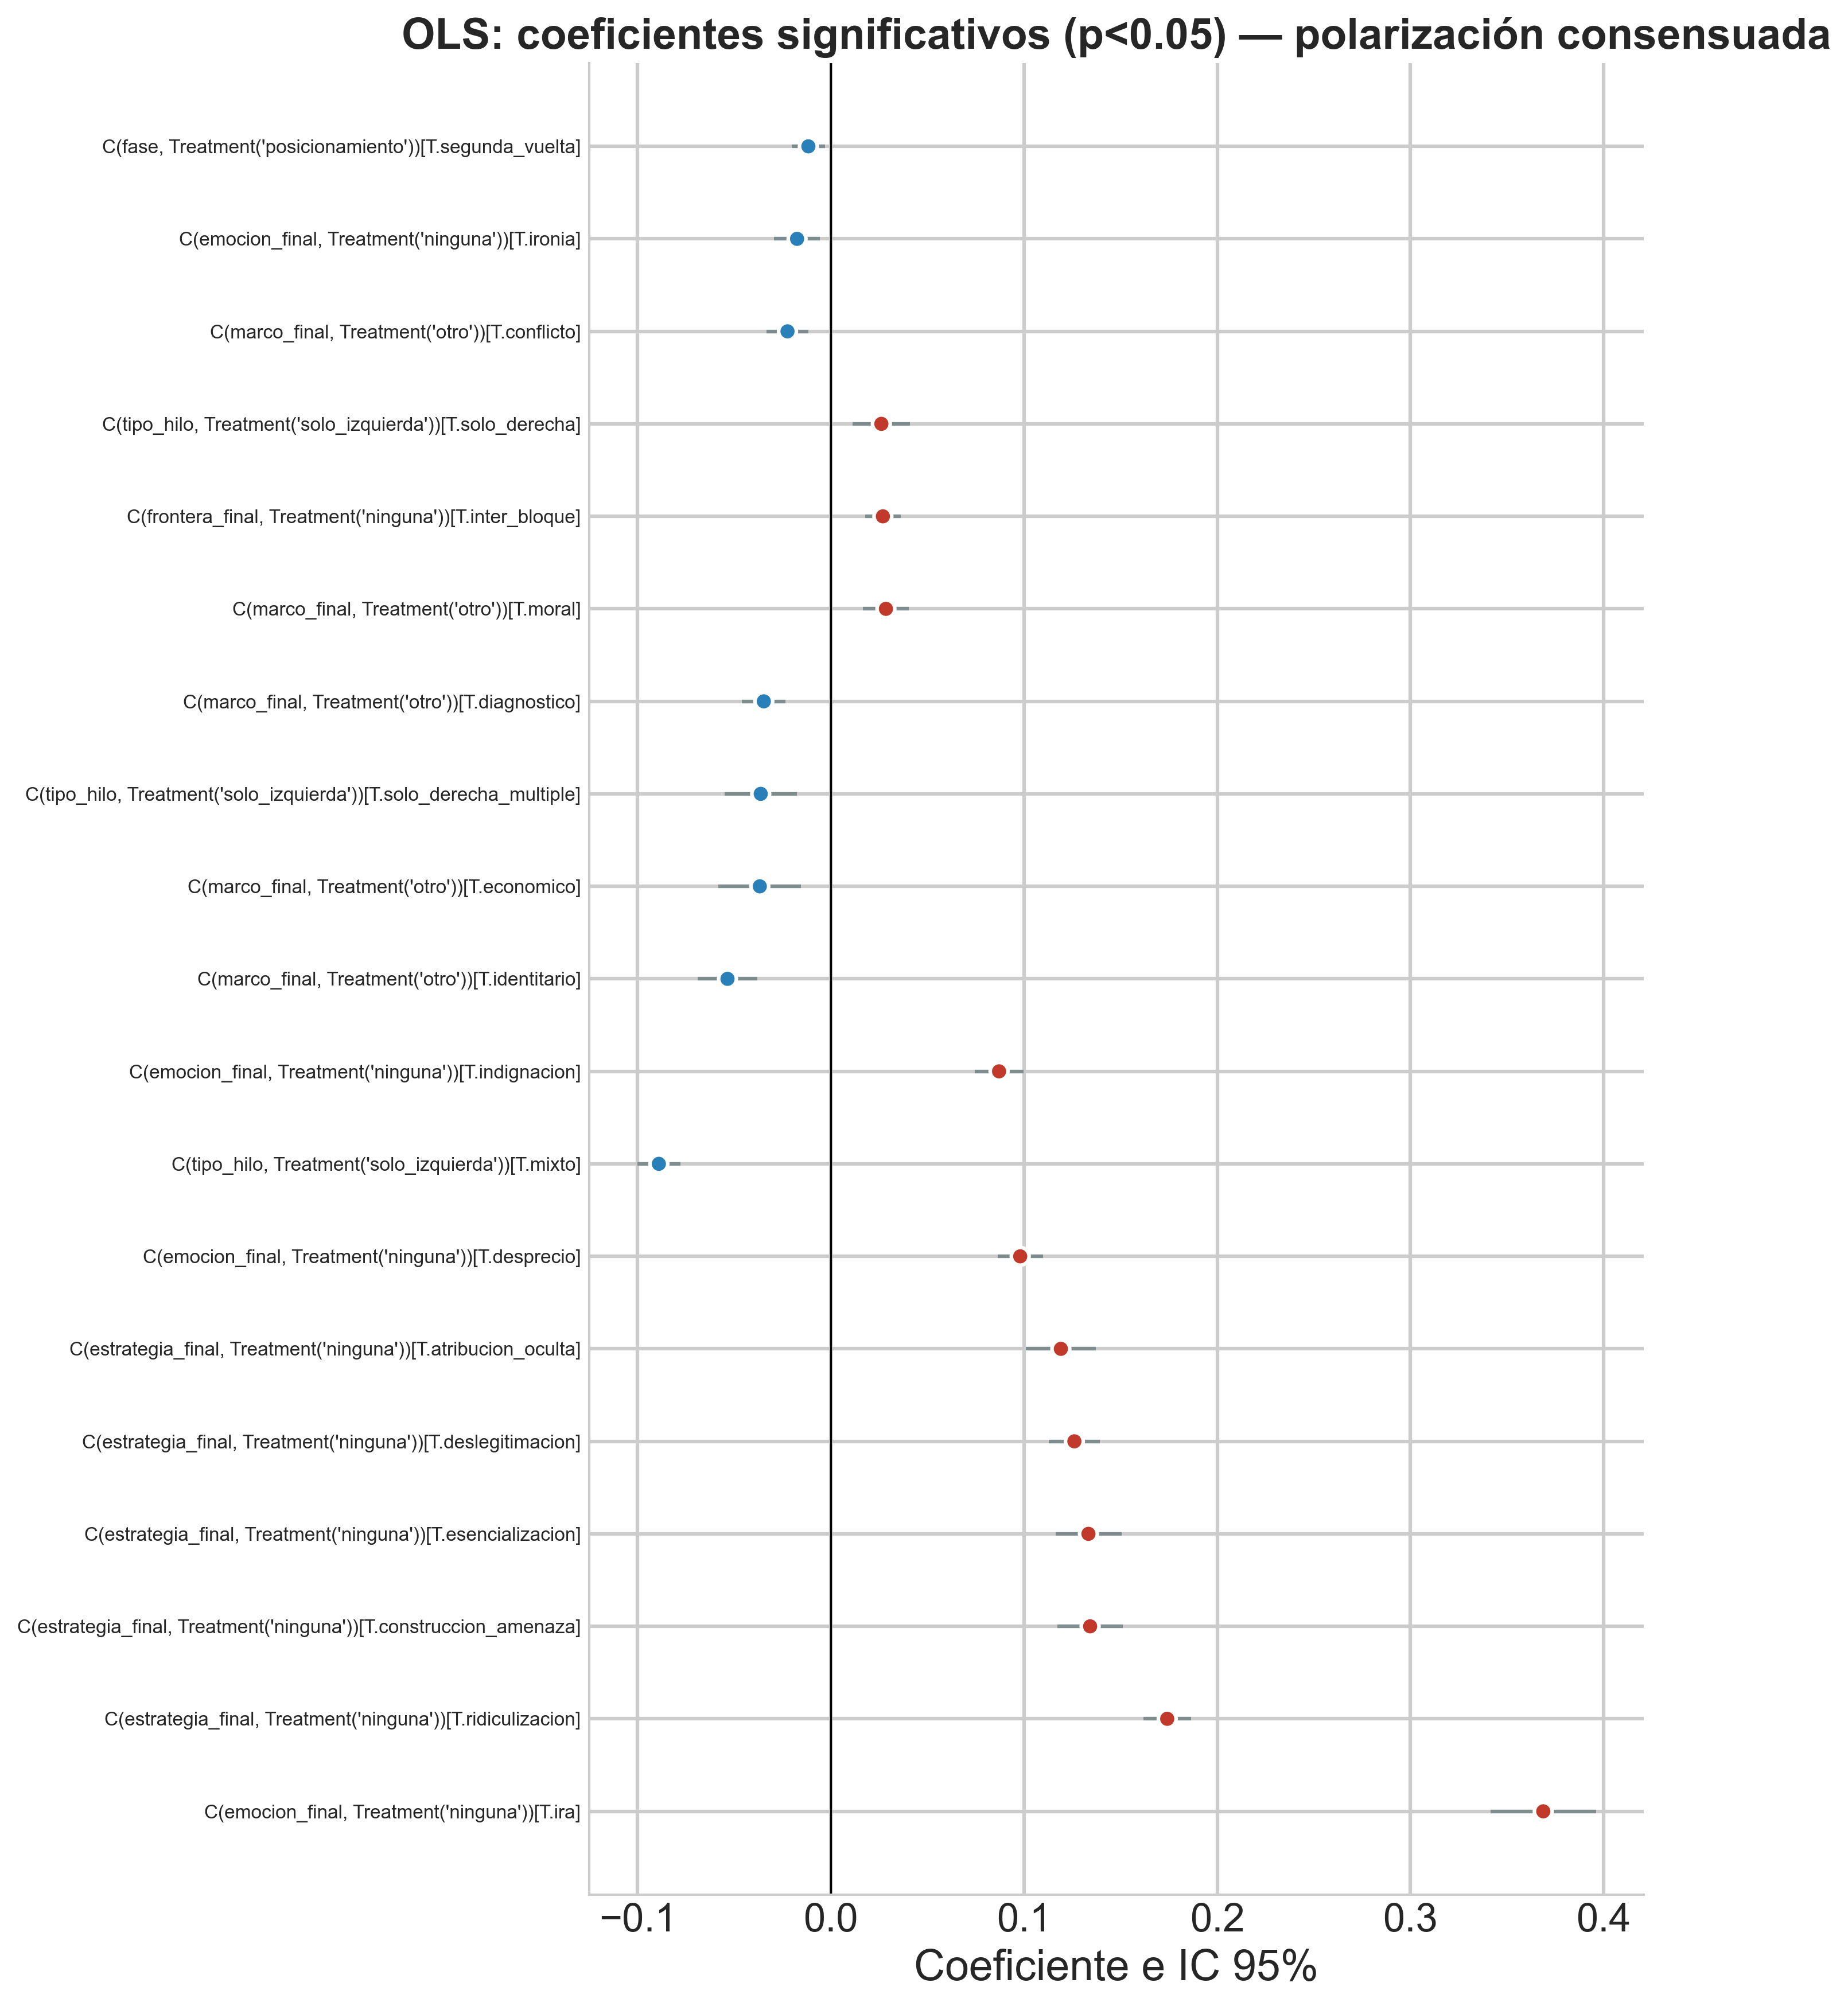
\includegraphics[width=0.82\textwidth,height=\textheight]{fig_thesis/coefplot_ols_polarizacion.png}

}

\caption{\label{fig-anexo-coefplot-ols}Coeficientes OLS para
polarización.}

\end{figure}%

\textbf{A.2 Interpretación de resultados (capítulo 8)}

\textbf{A.2.0 Diez combinaciones marco × emoción más frecuentes}

\begin{table}

\caption{\label{tbl-anexo-marco-emocion-top}Top 10 combinaciones marco ×
emoción.}

\centering{

[!h]
\centering
\resizebox{\ifdim\width>\linewidth\linewidth\else\width\fi}{!}{
\begin{tabular}{llrrr}
\toprule
Marco & Emoción & n & Prop. & Pol..med.\\
\midrule
\cellcolor{gray!10}{Conflicto} & \cellcolor{gray!10}{Desprecio} & \cellcolor{gray!10}{945} & \cellcolor{gray!10}{0.092} & \cellcolor{gray!10}{0.463}\\
Diagnóstico & Indignación & 844 & 0.082 & 0.430\\
\cellcolor{gray!10}{Conflicto} & \cellcolor{gray!10}{Indignación} & \cellcolor{gray!10}{758} & \cellcolor{gray!10}{0.074} & \cellcolor{gray!10}{0.448}\\
Conflicto & Ironía & 724 & 0.071 & 0.386\\
\cellcolor{gray!10}{Moral} & \cellcolor{gray!10}{Desprecio} & \cellcolor{gray!10}{702} & \cellcolor{gray!10}{0.069} & \cellcolor{gray!10}{0.541}\\
\addlinespace
Moral & Indignación & 627 & 0.061 & 0.503\\
\cellcolor{gray!10}{Diagnóstico} & \cellcolor{gray!10}{Desprecio} & \cellcolor{gray!10}{591} & \cellcolor{gray!10}{0.058} & \cellcolor{gray!10}{0.438}\\
Otro & Desprecio & 528 & 0.052 & 0.544\\
\cellcolor{gray!10}{Diagnóstico} & \cellcolor{gray!10}{Ninguna} & \cellcolor{gray!10}{463} & \cellcolor{gray!10}{0.045} & \cellcolor{gray!10}{0.261}\\
Otro & Ninguna & 435 & 0.042 & 0.296\\
\bottomrule
\multicolumn{5}{l}{\rule{0pt}{1em}\textit{Nota.} Pol. med.: polarización consensuada media en esa combinación. Mismos valores que en el análisis del capítulo 8.}\\
\end{tabular}}

}

\end{table}%

\begin{figure}[H]

\centering{

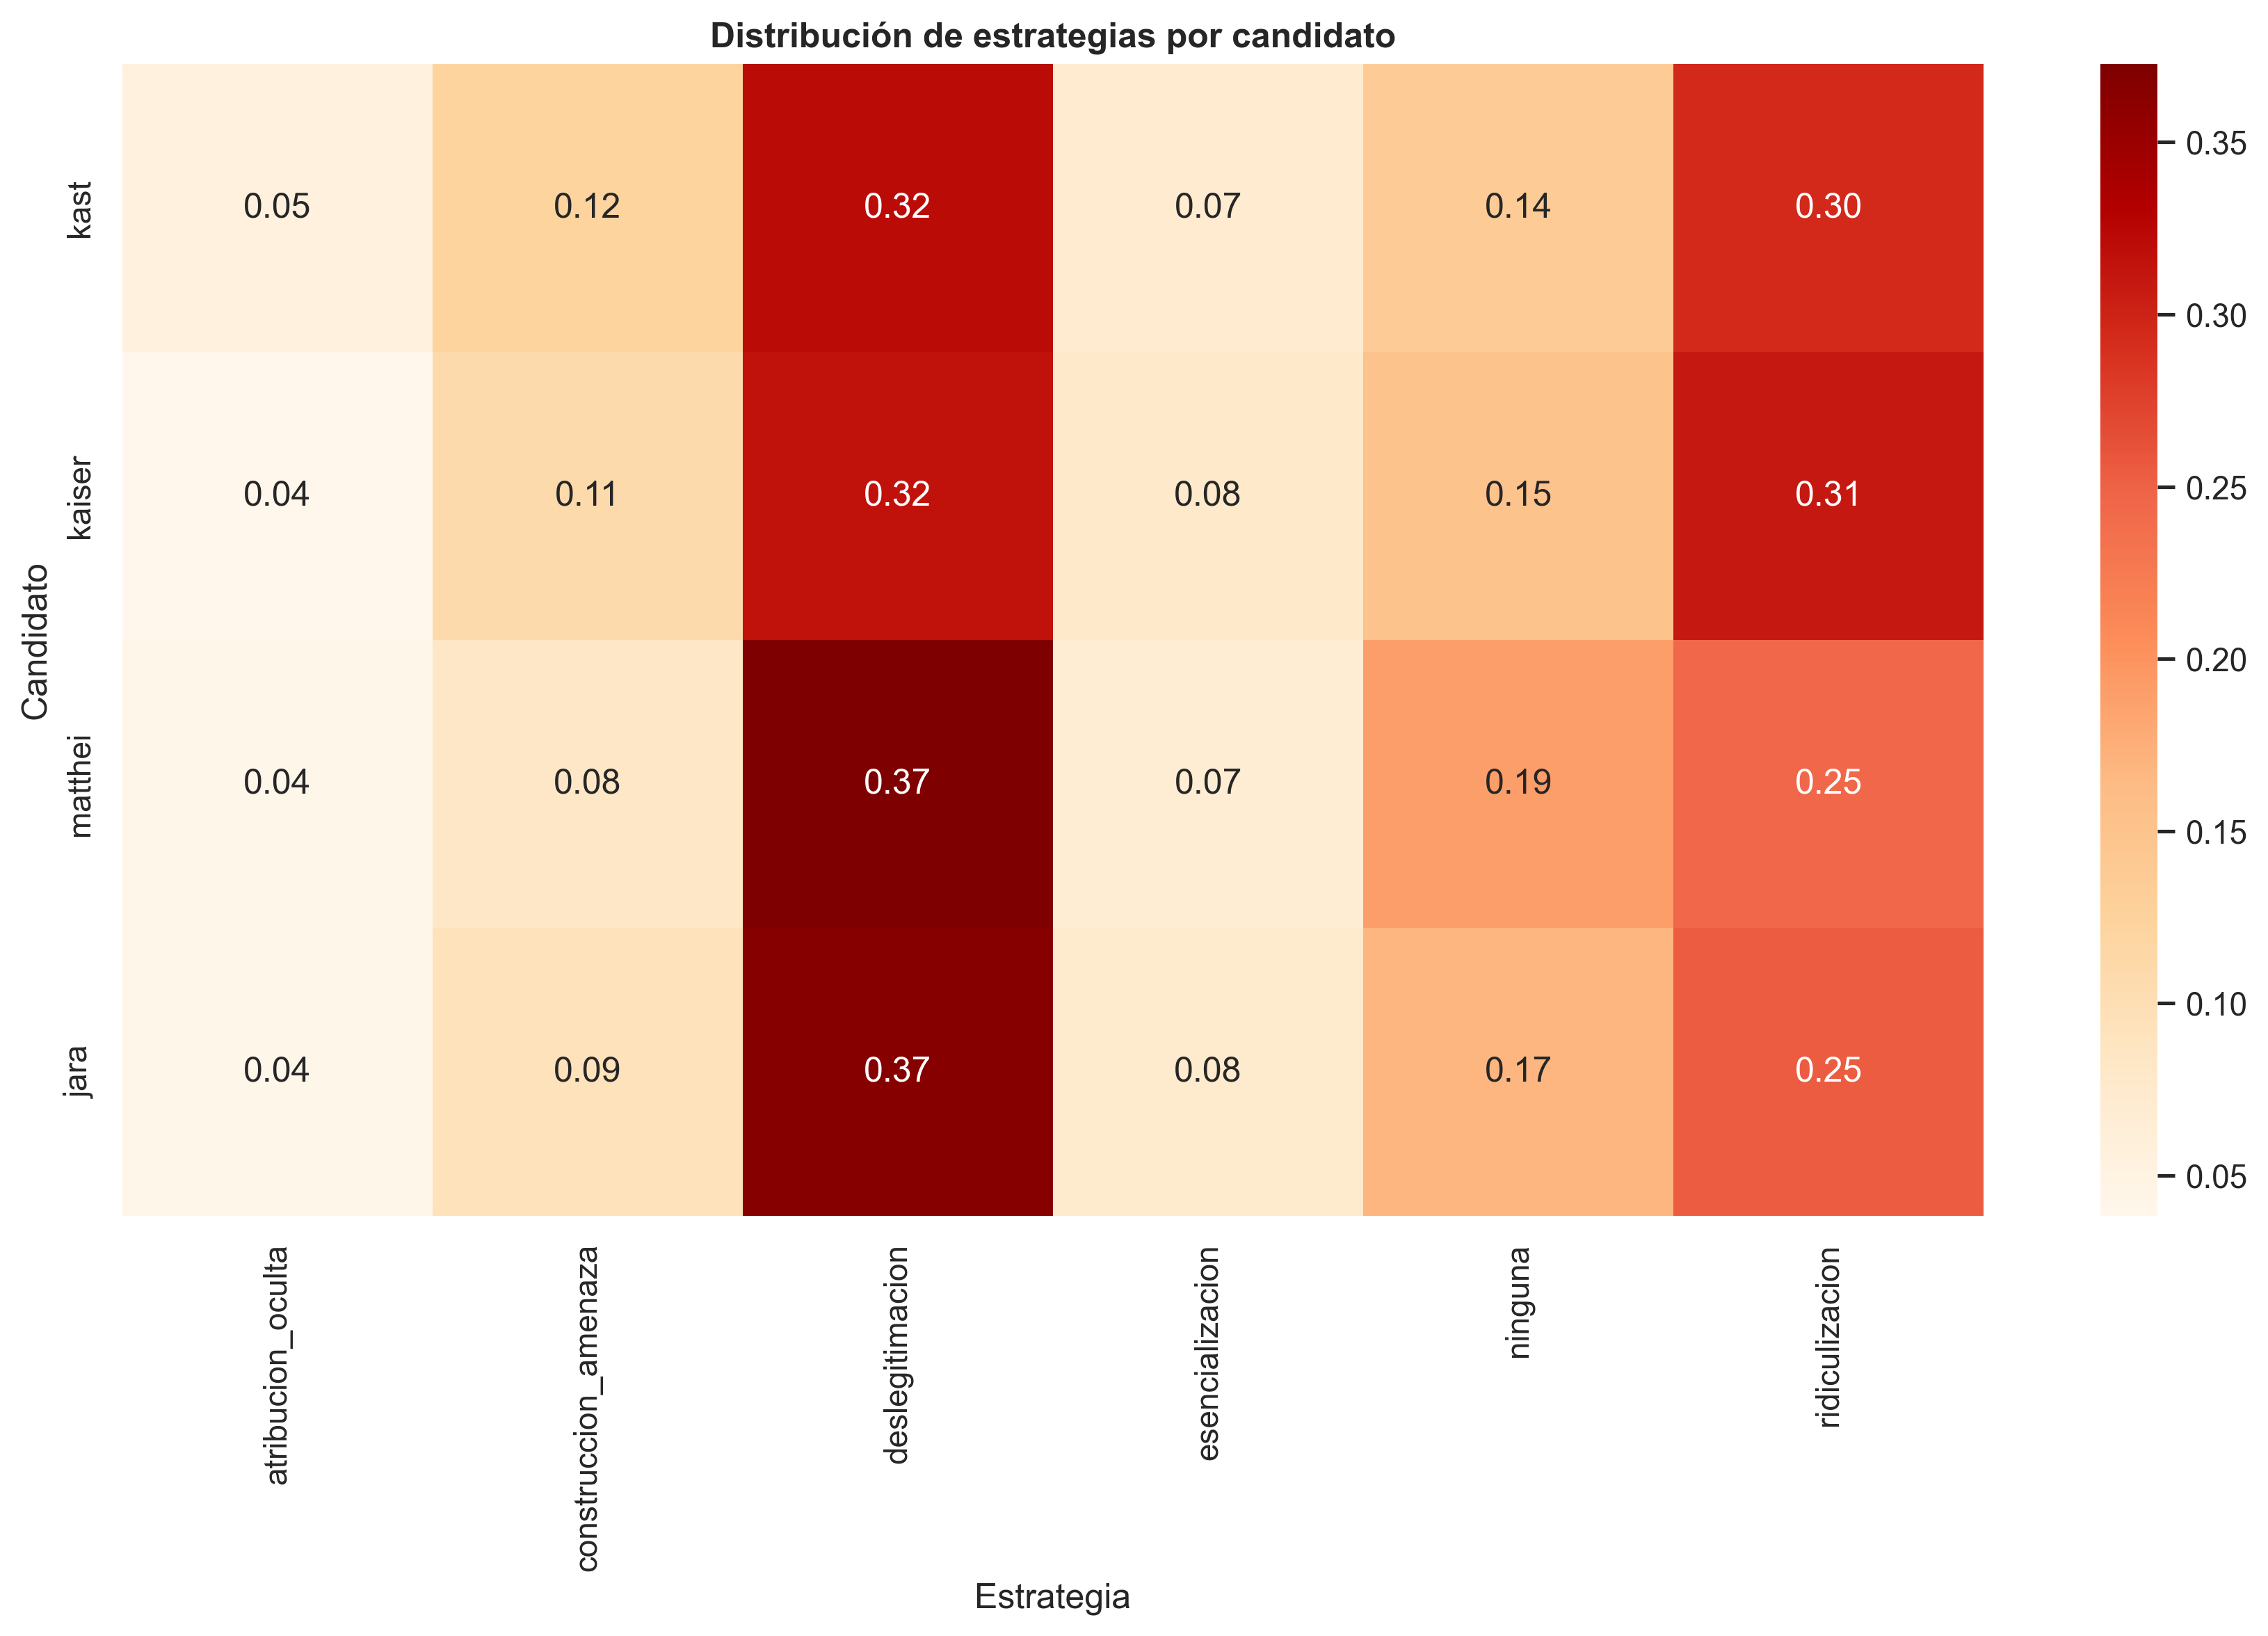
\includegraphics[width=0.82\textwidth,height=\textheight]{fig_thesis/distribucion_estrategias_candidato.png}

}

\caption{\label{fig-anexo-estrategias-candidato}Estrategias discursivas
por candidato objetivo.}

\end{figure}%

\textbf{A.2.1 Asociación marco × fase por candidato}

\begin{table}

\caption{\label{tbl-anexo-marcos-fase-candidato}Marco × fase por
candidato: chi-cuadrado y V de Cramér.}

\centering{

[!h]
\centering
\resizebox{\ifdim\width>\linewidth\linewidth\else\width\fi}{!}{
\begin{tabular}{lrlrr}
\toprule
Candidato & Chi-cuadrado & p & V de Cramér & N\\
\midrule
\cellcolor{gray!10}{kast} & \cellcolor{gray!10}{21.903} & \cellcolor{gray!10}{0.081} & \cellcolor{gray!10}{0.047} & \cellcolor{gray!10}{5052}\\
kaiser & 23.874 & 0.047 & 0.096 & 1308\\
\cellcolor{gray!10}{matthei} & \cellcolor{gray!10}{17.674} & \cellcolor{gray!10}{0.222} & \cellcolor{gray!10}{0.105} & \cellcolor{gray!10}{802}\\
jara & 31.817 & 0.004 & 0.072 & 3085\\
\bottomrule
\multicolumn{5}{l}{\rule{0pt}{1em}\textit{Nota.} p en formato APA. N = número de comentarios del candidato en el análisis.}\\
\end{tabular}}

}

\end{table}%

\textbf{A.2.2 Cruces de tono (posicionamiento → segunda vuelta; sin
neutro)}

\begin{table}

\caption{\label{tbl-anexo-cruce-sentimiento-pares-sv}Cruces de tono por
par de candidatos (sin neutro).}

\centering{

[!h]
\centering
\resizebox{\ifdim\width>\linewidth\linewidth\else\width\fi}{!}{
\begin{tabular}{lllr}
\toprule
Par & Origen (posicionamiento) & Tono en 2.ª vuelta (hacia Kast o Jara) & Probabilidad condicional (\%)\\
\midrule
\cellcolor{gray!10}{Jara → Kast} & \cellcolor{gray!10}{Jara: NEGATIVO} & \cellcolor{gray!10}{Kast: NEGATIVO} & \cellcolor{gray!10}{96.9}\\
Jara → Kast & Jara: NEGATIVO & Kast: POSITIVO & 3.1\\
\cellcolor{gray!10}{Jara → Kast} & \cellcolor{gray!10}{Jara: POSITIVO} & \cellcolor{gray!10}{Kast: NEGATIVO} & \cellcolor{gray!10}{100.0}\\
Kaiser → Jara & Kaiser: NEGATIVO & Jara: NEGATIVO & 85.7\\
\cellcolor{gray!10}{Kaiser → Jara} & \cellcolor{gray!10}{Kaiser: NEGATIVO} & \cellcolor{gray!10}{Jara: POSITIVO} & \cellcolor{gray!10}{14.3}\\
\addlinespace
Kaiser → Jara & Kaiser: POSITIVO & Jara: NEGATIVO & 100.0\\
\cellcolor{gray!10}{Kaiser → Kast} & \cellcolor{gray!10}{Kaiser: NEGATIVO} & \cellcolor{gray!10}{Kast: NEGATIVO} & \cellcolor{gray!10}{100.0}\\
Kaiser → Kast & Kaiser: POSITIVO & Kast: NEGATIVO & 100.0\\
\cellcolor{gray!10}{Kast → Jara} & \cellcolor{gray!10}{Kast: NEGATIVO} & \cellcolor{gray!10}{Jara: NEGATIVO} & \cellcolor{gray!10}{91.9}\\
Kast → Jara & Kast: NEGATIVO & Jara: POSITIVO & 8.1\\
\addlinespace
\cellcolor{gray!10}{Kast → Jara} & \cellcolor{gray!10}{Kast: POSITIVO} & \cellcolor{gray!10}{Jara: NEGATIVO} & \cellcolor{gray!10}{100.0}\\
Matthei → Jara & Matthei: NEGATIVO & Jara: NEGATIVO & 100.0\\
\cellcolor{gray!10}{Matthei → Jara} & \cellcolor{gray!10}{Matthei: POSITIVO} & \cellcolor{gray!10}{Jara: NEGATIVO} & \cellcolor{gray!10}{100.0}\\
Matthei → Kast & Matthei: NEGATIVO & Kast: NEGATIVO & 100.0\\
\cellcolor{gray!10}{Matthei → Kast} & \cellcolor{gray!10}{Matthei: POSITIVO} & \cellcolor{gray!10}{Kast: NEGATIVO} & \cellcolor{gray!10}{100.0}\\
\bottomrule
\end{tabular}}

}

\end{table}%

\textbf{A.2.3 Transiciones de tono hacia Kast (autores inicialmente
negativos)}

\begin{table}

\caption{\label{tbl-anexo-kast-transiciones}Transiciones de tono hacia
Kast (autores negativos iniciales).}

\centering{

[!h]
\centering
\resizebox{\ifdim\width>\linewidth\linewidth\else\width\fi}{!}{
\begin{tabular}{lr}
\toprule
Destino posterior (tono hacia Kast) & Porcentaje del total\\
\midrule
\cellcolor{gray!10}{Positivo} & \cellcolor{gray!10}{2.8}\\
Neutro & 9.8\\
\cellcolor{gray!10}{Negativo (persistencia)} & \cellcolor{gray!10}{87.4}\\
\bottomrule
\multicolumn{2}{l}{\rule{0pt}{1em}\textit{Nota.} Porcentajes calculados sobre el conjunto de autores con tono negativo hacia Kast en la fase inicial (N = 215). La columna indica qué fracción pasó a cada destino.}\\
\end{tabular}}

}

\end{table}%

\textbf{A.2.4 Cruces emocionales (posicionamiento → segunda vuelta; sin
«sin emoción»)}

\begin{table}

\caption{\label{tbl-anexo-cruce-emocion-sin-se-pares-sv}Cruces
emocionales por par de candidatos (sin «sin emoción»).}

\centering{

[!h]
\centering
\resizebox{\ifdim\width>\linewidth\linewidth\else\width\fi}{!}{
\begin{tabular}{lllr}
\toprule
Par & Emoción grupo (hacia candidato origen, posicionamiento) & Destino (2.ª vuelta: hacia candidato destino) & Probabilidad condicional (\%)\\
\midrule
\cellcolor{gray!10}{Jara → Kast} & \cellcolor{gray!10}{hostilidad} & \cellcolor{gray!10}{Kast: hostilidad} & \cellcolor{gray!10}{71.2}\\
Jara → Kast & hostilidad & Kast: ironía & 20.3\\
\cellcolor{gray!10}{Jara → Kast} & \cellcolor{gray!10}{hostilidad} & \cellcolor{gray!10}{Kast: miedo} & \cellcolor{gray!10}{5.1}\\
Jara → Kast & hostilidad & Kast: positivo & 3.4\\
\cellcolor{gray!10}{Jara → Kast} & \cellcolor{gray!10}{ironía} & \cellcolor{gray!10}{Kast: hostilidad} & \cellcolor{gray!10}{82.4}\\
\addlinespace
Jara → Kast & ironía & Kast: ironía & 11.8\\
\cellcolor{gray!10}{Jara → Kast} & \cellcolor{gray!10}{ironía} & \cellcolor{gray!10}{Kast: miedo} & \cellcolor{gray!10}{5.9}\\
Jara → Kast & miedo & Kast: hostilidad & 50.0\\
\cellcolor{gray!10}{Jara → Kast} & \cellcolor{gray!10}{miedo} & \cellcolor{gray!10}{Kast: ironía} & \cellcolor{gray!10}{50.0}\\
Jara → Kast & otro & Kast: positivo & 100.0\\
\addlinespace
\cellcolor{gray!10}{Jara → Kast} & \cellcolor{gray!10}{positivo} & \cellcolor{gray!10}{Kast: hostilidad} & \cellcolor{gray!10}{100.0}\\
Kaiser → Jara & hostilidad & Jara: hostilidad & 62.5\\
\cellcolor{gray!10}{Kaiser → Jara} & \cellcolor{gray!10}{hostilidad} & \cellcolor{gray!10}{Jara: ironía} & \cellcolor{gray!10}{37.5}\\
Kaiser → Jara & ironía & Jara: hostilidad & 20.0\\
\cellcolor{gray!10}{Kaiser → Jara} & \cellcolor{gray!10}{ironía} & \cellcolor{gray!10}{Jara: ironía} & \cellcolor{gray!10}{60.0}\\
\addlinespace
Kaiser → Jara & ironía & Jara: positivo & 20.0\\
\cellcolor{gray!10}{Kaiser → Kast} & \cellcolor{gray!10}{hostilidad} & \cellcolor{gray!10}{Kast: hostilidad} & \cellcolor{gray!10}{77.8}\\
Kaiser → Kast & hostilidad & Kast: ironía & 11.1\\
\cellcolor{gray!10}{Kaiser → Kast} & \cellcolor{gray!10}{hostilidad} & \cellcolor{gray!10}{Kast: positivo} & \cellcolor{gray!10}{11.1}\\
Kaiser → Kast & ironía & Kast: hostilidad & 60.0\\
\addlinespace
\cellcolor{gray!10}{Kaiser → Kast} & \cellcolor{gray!10}{ironía} & \cellcolor{gray!10}{Kast: ironía} & \cellcolor{gray!10}{40.0}\\
Kast → Jara & hostilidad & Jara: hostilidad & 66.1\\
\cellcolor{gray!10}{Kast → Jara} & \cellcolor{gray!10}{hostilidad} & \cellcolor{gray!10}{Jara: ironía} & \cellcolor{gray!10}{29.0}\\
Kast → Jara & hostilidad & Jara: miedo & 1.6\\
\cellcolor{gray!10}{Kast → Jara} & \cellcolor{gray!10}{hostilidad} & \cellcolor{gray!10}{Jara: positivo} & \cellcolor{gray!10}{3.2}\\
\addlinespace
Kast → Jara & ironía & Jara: hostilidad & 42.9\\
\cellcolor{gray!10}{Kast → Jara} & \cellcolor{gray!10}{ironía} & \cellcolor{gray!10}{Jara: ironía} & \cellcolor{gray!10}{28.6}\\
Kast → Jara & ironía & Jara: miedo & 28.6\\
\cellcolor{gray!10}{Kast → Jara} & \cellcolor{gray!10}{miedo} & \cellcolor{gray!10}{Jara: hostilidad} & \cellcolor{gray!10}{100.0}\\
Matthei → Jara & hostilidad & Jara: hostilidad & 57.1\\
\addlinespace
\cellcolor{gray!10}{Matthei → Jara} & \cellcolor{gray!10}{hostilidad} & \cellcolor{gray!10}{Jara: ironía} & \cellcolor{gray!10}{14.3}\\
Matthei → Jara & hostilidad & Jara: miedo & 14.3\\
\cellcolor{gray!10}{Matthei → Jara} & \cellcolor{gray!10}{hostilidad} & \cellcolor{gray!10}{Jara: positivo} & \cellcolor{gray!10}{14.3}\\
Matthei → Jara & ironía & Jara: ironía & 66.7\\
\cellcolor{gray!10}{Matthei → Jara} & \cellcolor{gray!10}{ironía} & \cellcolor{gray!10}{Jara: miedo} & \cellcolor{gray!10}{33.3}\\
\addlinespace
Matthei → Jara & positivo & Jara: hostilidad & 100.0\\
\cellcolor{gray!10}{Matthei → Kast} & \cellcolor{gray!10}{hostilidad} & \cellcolor{gray!10}{Kast: hostilidad} & \cellcolor{gray!10}{77.8}\\
Matthei → Kast & hostilidad & Kast: ironía & 11.1\\
\cellcolor{gray!10}{Matthei → Kast} & \cellcolor{gray!10}{hostilidad} & \cellcolor{gray!10}{Kast: positivo} & \cellcolor{gray!10}{11.1}\\
Matthei → Kast & ironía & Kast: hostilidad & 75.0\\
\addlinespace
\cellcolor{gray!10}{Matthei → Kast} & \cellcolor{gray!10}{ironía} & \cellcolor{gray!10}{Kast: ironía} & \cellcolor{gray!10}{25.0}\\
\bottomrule
\end{tabular}}

}

\end{table}%

\bookmarksetup{startatroot}

\chapter{Referencias}\label{referencias}

\phantomsection\label{refs}
\begin{CSLReferences}{1}{0}
\bibitem[\citeproctext]{ref-Lazer2009}
Lazer. 2009. {``Lazer2009.''}

\bibitem[\citeproctext]{ref-Salganik2019}
Salganik. 2019. {``Salganik2019.''}

\bibitem[\citeproctext]{ref-Zimmer2017}
Zimmer. 2017. {``Zimmer2017.''}

\end{CSLReferences}




\end{document}
